% !TEX program = xelatex
% !TeX encoding = utf8
% !TeX spellcheck = pl-PL

%%%%%%%%%%%%%%%%%%%%%%%%%%%%%%%%%%%%%%%%%%%%%%%%%%%%%%%%%%%%%%%%%%%%%%%%%%%
% Wybierz rodzaj pracy dyplomowej oraz wydział
% Pick thesis type and faculty
%%%%%%%%%%%%%%%%%%%%%%%%%%%%%%%%%%%%%%%%%%%%%%%%%%%%%%%%%%%%%%%%%%%%%%%%%%%
\documentclass[thesis=mgr,faculty=gik]{EE-dyplom} 

% thesis=[inz|mgr|bsc|msc]
%  * inz - praca inżynierska
%  * mgr - praca magisterska
%  * bsc - bachelor thesis
%  * msc - master thesis

% Skróty nazw wydziałów zgodne z domenami internetowymi
% Abbreviations of Faculties according to Internet subdomains
% faculty=[
%	arch,
%	gik,
%	ee,
%	wip
%	]

%%%%%%%%%%%%%%%%%%%%%%%%%%%%%%%%%%%%%%%%%%%%%%%%%%%%%%%%%%%%%%%%%%%%%%%%%%%
% Konfiguracja - do personalizacji
% Configuration - to be personalized
%%%%%%%%%%%%%%%%%%%%%%%%%%%%%%%%%%%%%%%%%%%%%%%%%%%%%%%%%%%%%%%%%%%%%%%%%%%
\instytut{Instytut Automatyki i Robotyki}
\kierunek{Automatyka, Robotyka i Informatyka Przemysłowa}
% \specjalnosc{Rzeczowidztwo}
\title{Przygotowanie zbioru danych wejściowych do opracowania modelu do predykcji cen energii elektrycznej na rynku dnia następnego w Polsce}
\engtitle{Preparation of an input dataset for the development of a model for the prediction of electricity prices in the day-ahead market in Poland}
\album{335662}
\author{inż. Ivan Kaliankovich}
\promotor{prof. dr inż. Paweł Wnuk}
\date{2025}
\longdate{2025-05-01}

\streszczeniepracy{
Niniejsza praca poświęcona jest analizie i prognozowaniu cen energii elektrycznej na Rynku Dnia Następnego w Polsce w latach 2016-2023. Badanie skupia się na zrozumieniu dynamiki cen na tym rynku, który odgrywa kluczową rolę w zarządzaniu systemem elektroenergetycznym, umożliwiając elastyczne dostosowanie podaży do popytu w krótkim horyzoncie czasowym. Centralnym elementem pracy jest przygotowanie kompleksowej bazy danych, która obejmuje zarówno okresy stabilności cenowej, jak i momenty wysokiej zmienności, wynikające z czynników ekonomicznych, geopolitycznych oraz pogodowych. Uwzględniono szeroki zestaw danych, takich jak historyczne ceny energii, zapotrzebowanie, generacja energii z odnawialnych źródeł, ceny paliw, emisje CO$_2$, a także warunki atmosferyczne, co pozwoliło na holistyczne podejście do analizy.

Dobór zmiennych do analizy został oparty na gruntownym przeglądzie literatury, który wskazał na znaczenie takich czynników, jak opóźnione ceny energii, zapotrzebowanie systemowe, generacja energii odnawialnej oraz zmienne sezonowe i ekonomiczne, w tym efekty kalendarzowe i wahania cen surowców. Uwzględnienie tych aspektów umożliwiło dostosowanie badania do specyficznych uwarunkowań polskiego rynku energii, który charakteryzuje się unikalnymi wyzwaniami, takimi jak zależność od tradycyjnych źródeł energii i rosnąca rola odnawialnych źródeł energii. Analiza została przeprowadzona w dwóch różnych okresach, co pozwoliło na ocenę skuteczności stosowanych metod w zróżnicowanych warunkach rynkowych, od stabilnych po te o dużej niestabilności.

W badaniu wykorzystano zarówno modele statystyczne, jak i techniki uczenia maszynowego, dostosowując ich parametry, aby zwiększyć zdolność do przewidywania cen. Wyniki poddano ocenie za pomocą standardowych miar, analizując wpływ różnych zmiennych na jakość prognoz oraz porównując efektywność modeli w zależności od użytych danych. Praca rzuca światło na trudności związane z prognozowaniem w niestabilnych warunkach rynkowych, szczególnie w kontekście nagłych zmian cen wywołanych czynnikami zewnętrznymi, i wskazuje na konieczność dalszego rozwoju zaawansowanych metod analitycznych, takich jak podejścia hybrydowe, które lepiej radzą sobie z nieliniowością danych. Opracowanie może stanowić wsparcie dla uczestników rynku energii w podejmowaniu decyzji handlowych, zarządzaniu ryzykiem finansowym oraz planowaniu strategii w dynamicznie zmieniającym się środowisku energetycznym.
}

\slowakluczowe{Rynek Dnia Następnego, prognozowanie cen energii, zbiór danych}

\thesisabstract{
The following study focuses on the analysis and forecasting of electricity prices on the Day-Ahead Market in Poland over the period 2016-2023. The study aims to understand the price dynamics on this market, which plays a crucial role in managing the power system by enabling flexible adjustments of supply to demand in the short term. A central element of the research is the development of a comprehensive database covering both periods of price stability and high volatility, driven by economic, geopolitical, and weather-related factors. The dataset includes a wide range of variables such as historical electricity prices, demand, generation from renewable energy sources, fuel prices, CO$_2$ emissions, and weather conditions, facilitating a holistic approach to the analysis.

The selection of variables was guided by an in-depth literature review, highlighting the importance of factors such as lagged energy prices, system demand, renewable energy generation, and seasonal and economic variables, including calendar effects and raw material price fluctuations. Incorporating these aspects allowed the study to address the specific conditions of the Polish energy market, which faces unique challenges, such as reliance on traditional energy sources and the growing role of renewables. The analysis was conducted across two distinct periods, enabling an evaluation of model performance under varying market conditions, from stable to highly volatile.

The study employed both statistical models and machine learning techniques, adjusting their parameters to enhance predictive capabilities. The results were assessed using standard metrics, analyzing the impact of different variables on forecast accuracy and comparing model effectiveness based on the datasets used. The work sheds light on the challenges of forecasting in unstable market conditions, particularly in the context of sudden price changes triggered by external factors, and underscores the need for further development of advanced analytical methods, such as hybrid approaches, which better handle data nonlinearity. This research may support market participants in making trading decisions, managing financial risk, and planning strategies in a dynamically changing energy environment.
}

\thesiskeywords{Day-Ahead Market, electricity price forecasting, dataset}

\usepackage{float}
\makeglossaries

\begin{document}
    \frontpages % Strony nagłówkowe

    \chapter{Wstep}

\subsection*{Wprowadzenie}
\label{ch:wprowadzenie}
Rynek energii elektrycznej to jeden z filarów współczesnej gospodarki, a jego sprawne funkcjonowanie ma kluczowe znaczenie dla stabilności systemów elektroenergetycznych, przedsiębiorstw i codziennego życia konsumentów. W centrum rynku znajduje się \gls{rdn}, który działa jako platforma handlu energią na dzień przed jej dostarczeniem. RDN jest miejscem, gdzie producenci energii od elektrowni węglowych po farmy wiatrowe spotykają się z odbiorcami, takimi jak dostawcy energii dla domów mieszkalnych czy duże zakłady przemysłowe, w celu ustalenia ceny i wolumenów energii na każdą godzinę kolejnego dnia. Mechanizm działania RDN opiera się na systemie aukcyjnym: uczestnicy składają oferty kupna i sprzedaży, określając, ile energii są w stanie dostarczyć lub kupić oraz po jakiej cenie. System następnie dopasowuje te oferty, ustalając cenę równowagi, która obowiązuje dla danej godziny \cite{maciejowska2022forecastingelectricityprices}.

Taki model handlu pozwala na elastyczne reagowanie na zmieniające się warunki - zarówno po stronie podaży, jak i popytu. Na przykład, jeśli prognozy wskazują na silny wiatr, producenci energii wiatrowej mogą zwiększyć podaż, co może obniżyć ceny; z kolei fala upałów może zwiększyć zapotrzebowanie na energię do klimatyzacji, podnosząc ceny. RDN działa w wielu krajach, choć jego specyfika różni się w zależności od regionu. W Europie, w tym w Polsce, rynek ten jest częścią szerszego systemu integracji rynków energii, który ma na celu zapewnienie płynności i efektywności handlu. W Stanach Zjednoczonych RDN funkcjonuje w ramach regionalnych rynków, takich jak PJM Interconnection czy California ISO (CAISO), gdzie handel energią jest dodatkowo skomplikowany przez różnice regulacyjne między stanami. Niezależnie od regionu, RDN jest kluczowym narzędziem w zarządzaniu systemem elektroenergetycznym, umożliwiając szybkie dostosowanie podaży do popytu w krótkim horyzoncie czasowym \cite{maciejowska2022forecastingelectricityprices}.

Jednak handel na RDN to nie tylko szansa na zysk dla wszystkich biorących udział, ale i ogromne ryzyko finansowe, które wynika z nieprzewidywalności cen energii. Na rynku amerykańskim, gdzie mechanizm licytacji między kupującymi (buyers) a sprzedającymi (sellers) jest szczególnie rozwinięty, ryzyko to jest wyjątkowo widoczne. Uczestnicy rynku muszą składać oferty w czasie rzeczywistym, próbując przewidzieć, jak zachowa się cena w danej godzinie. Jeśli producent energii zaoferuje zbyt wysoką cenę, jego energia może nie zostać kupiona, co oznacza utratę przychodów; z kolei kupujący, który zaoferuje zbyt niską cenę, może zostać zmuszony do zakupu energii po znacznie wyższej cenie rynkowej. Przykładem skali tego ryzyka jest kryzys w Teksasie w lutym 2021 roku \cite{BUSBY2021102106}. W wyniku ekstremalnych mrozów i awarii systemu elektroenergetycznego ceny na rynku ERCOT (Electric Reliability Council of Texas) wzrosły do 9000 USD/MWh - poziomu, który dla wielu uczestników rynku oznaczał straty liczone w dziesiątkach milionów dolarów. W takich warunkach dokładna predykcja cen staje się nie tylko narzędziem do optymalizacji handlu, ale wręcz koniecznością, by uniknąć katastrofalnych strat. Na rynkach krajów rozwiniętych, gdzie \gls{oze} odgrywają coraz większą rolę, ceny mogą spadać do wartości ujemnych w godzinach nadprodukcji np. z energii słonecznej, by kilka godzin później gwałtownie wzrosnąć, gdy zapotrzebowanie przewyższa podaż. Ta zmienność sprawia, że handel na RDN przypomina grę o wysoką stawkę, w której każdy ruch musi być dokładnie przemyślany.

Rynek bilansujący stanowi kolejny istotny element systemu elektroenergetycznego, uzupełniając funkcjonowanie RDN. Działa on w czasie rzeczywistym, umożliwiając operatorom systemu elektroenergetycznego (w Polsce jest to Polskie Sieci Elektroenergetyczne, PSE \cite{PSE_BALANCING_MARKET}) równoważenie podaży i popytu w sytuacjach, gdy rzeczywiste zużycie energii odbiega od prognoz ustalanych na RDN. Na rynku bilansującym uczestnicy mogą zgłaszać oferty na dostawy energii w bardzo krótkim horyzoncie czasowym, nawet w ciągu kilkunastu minut, co pozwala na szybkie reagowanie na nagłe zmiany, takie jak awarie elektrowni, nieoczekiwane skoki zapotrzebowania czy zmienność produkcji z OZE. Ceny na rynku bilansującym są często bardziej zmienne niż na RDN, co dodatkowo zwiększa ryzyko finansowe dla uczestników, ale jednocześnie podkreśla znaczenie precyzyjnych prognoz cen, które mogą pomóc w lepszym zarządzaniu tymi krótkoterminowymi wahaniami.

W niniejszej pracy magisterskiej skupiam się na analizie RDN w Polsce, który choć różni się od rynku amerykańskiego pod względem skali i regulacji, również zmaga się z podobnymi wyzwaniami. W Europie, w tym w Polsce, RDN jest częścią zintegrowanego systemu handlu energią, który opiera się na współpracy między krajami i dąży do harmonizacji rynków energii w ramach Unii Europejskiej. Mechanizm ustalania cen na RDN w Polsce opiera się na zasadzie jednolitej ceny, gdzie cena rozliczeniowa jest wyznaczana na podstawie równowagi popytu i podaży dla każdej godziny. Oznacza to, że wszyscy uczestnicy, których oferty zostały zaakceptowane, rozliczają się po tej samej cenie, co zapewnia przejrzystość i efektywność handlu. W Polsce RDN jest prowadzony przez Towarową Giełdę Energii (TGE), która od 2000 roku pełni rolę kluczowej platformy handlu energią. TGE organizuje aukcje na RDN, umożliwiając uczestnikom składanie ofert na każdą godzinę kolejnego dnia.W latach 2016-2023, które obejmują analizowany w pracy okres, ceny na RDN w Polsce wahały się od 200 PLN/MWh aż do ponad 3000 PLN/MWh, co odzwierciedla zarówno lokalne uwarunkowania (np. zależność od węgla, rosnąca rola OZE), jak i globalne trendy. Ważną rolą w takiej zmienności odegrały także niespodziewane czynniki zewnętrzne, zwane czarnymi łąbędziami. Z przykładów takich czynników można wymienić wybuch pandemii i wprowadzenie w związku z tym restrykcji na pracę oraz kryzys energetyczny w 2022 roku wywołany konfliktem zbrojnym na Ukrainie. Wszystkie te czynniki sprawiają, że prognozowanie cen energii elektrycznej na RDN w Polsce staje się niezwykle złożonym zadaniem, które wymaga uwzględnienia wielu zmiennych i zastosowania zaawansowanych metod analizy danych.

\subsection*{Cel pracy}
\label{ch:cel_pracy}

Większość dotychczasowych badań w literaturze naukowej dotycząca prognozowania cen energii elektrycznej, skupia się głównie na rynkach amerykańskich, europejskich oraz azjatyckich, pomijając specyfikę polskiego rynku energii. W związku z tym, celem niniejszej pracy jest opracowanie obszernej bazy danych z polskiego rynku energii, obejmującej zarówno okres umiarkowanej zmienności cen, jak i okres dużej zmienności cen i brak stabilności rynkowej. Baza danych zostanie przygotowana w celu uwzględnienia kluczowych czynników wpływających na ceny energii elektrycznej, charakterystycznych dla polskiego rynku. Następnie, w celu przetestowania użyteczności opracowanej bazy danych, przeprowadzono analizę z wykorzystaniem wybranych modeli uczenia maszynowego: regresji liniowej, regresji grzbietowej, modelu Prophet oraz wielowarstwowej sieci neuronowej.
    \makeatletter
    \@openrightfalse
    \makeatother
    \chapter{Przegląd literatury}
\label{ch:literatura}
Rozdział przedstawia przegląd literatury dotyczącej prognozowania cen energii elektrycznej, ze szczególnym uwzględnieniem zmiennych wejściowych oraz zwykle używanych modeli prognozowania. W analizie odwołano się zarówno do prac profesora Rafała Werona z Politechniki Wrocławskiej, który jest uznanym ekspertem w dziedzinie EPF, jak i do badań innych autorów, aby zapewnić kompleksowy kontekst dla przeprowadzonego badania.

\section{Zmienne wejściowe}
\label{sec:zmienne_wejsciowe_literatura}

W przeglądzie literatury dotyczącym prognozowania cen energii elektrycznej na rynkach dnia następnego, artykuł napisany przez Jesus Lago o współautorstwie prof. Werona \cite{LAGO2021116983} może stanowić istotny punkt odniesienia pod względem wyboru zmiennych wejściowych. Autorzy przyjęli zestaw dostępnych danych wejściowych dla prognozowania godzinowych cen na rynkach energii elektrycznej Nord Pool, EPEX-BE, EPEX-FR, EPEX-DE oraz PJM.
Niezależnie od zastosowanych przez autorów modeli (LEAR czy DNN), dla wszystkich rynków stworzono wektory zawierające po 24 wartości odpowiadające każdej godzinie dla cen z poprzednich trzech dni oraz tygodnia wstecz. Do tych wektorów dodano wektor określający dzień tygodnia w celu uwzględnienia sezonowości dziennej. Dodatkowo pod uwagę wzięto zmienne fundamentalne, różniące się w zależności od analizowanego rynku. \newline
Dla rynku Nord Pool (NP) były to prognozy zapotrzebowania na moc oraz generacji energii wiatrowej.\newline
Dla rynku PJM w Stanach Zjednoczonych uwzględniono dwie serie prognoz zapotrzebowania na moc: prognozę zapotrzebowania dla całego systemu oraz prognozę dla strefy Commonwealth Edison.\newline
Dla rynku EPEX-BE w Belgii wykorzystano prognozę zapotrzebowania na moc we Francji oraz prognozę generacji we Francji, ponieważ wcześniejsze badania wykazują, że właśnie te dwie zmienne są najlepszymi predyktorami cen belgijskich. \newline
Dla rynku EPEX-FR we Francji brano pod uwagę prognozę zapotrzebowania na moc oraz prognozę generacji.\newline
Dla rynku EPEX-DE w Niemczech uwzględniono prognozę zapotrzebowania na moc oraz zagregowane prognozy generacji energii wiatrowej i słonecznej.\newline
Do wszystkich wymienionych zmiennych fundamentalnych dodano wektory godzinowe tych zmiennych na dzień oraz tydzień wstecz.

Kolejnym artykułem wartym uwagi jest artykuł skupiony na postprocesingu \cite{LIPIECKI2024107934} w prognozowaniu cen energii elektrycznej metodami probabilistycznymi. Do osiągnięcia celu zostały wykorzystane następujące zmienne: 
\begin{itemize}
    \item Historyczne ceny energii elektrycznej z poprzednich jednego, dwóch, trzech i siedmiu dni
    \item Prognoza systemowego zapotrzebowania na moc
    \item Prognoza generacji energii z odnawialnych źródeł będąca sumą prognoz generacji energii wiatrowej i słonecznej
    \item Ceny uprawnień do emisji dwutlenku węgla
    \item Ceny gazu ziemnego
    \item Ceny ropy naftowej Brent
    \item Cena emisji węgla
    \item Zmienne czasowe reprezentujące dni tygodnia
    \item Zmienne czasowe, czyli zmienne binarne reprezentujące dni tygodnia
\end{itemize}
Warto podkreślić, że autorzy zastosowali transformację hiperbolicznego sinusa do cen energii elektrycznej w celu stabilizacji wariancji przed modelowaniem.

W innym artykule o współautorstwie prof. Werona \cite{en9080621} podkreśla się, że opóźnione ceny oraz zmienne egzogeniczne określające obciążenie systemowe oraz strefowe mają bardzo istotny wpływ na prognozowanie cen.

Artykuł prof. Ziel \cite{ZIEL201598} analizujący niemiecki RDN, potwierdza poprzednie tezy, wskazując na znaczenie cen energii opóźnionych, obciążenia sieci i energii z OZE. Opisujący przez niego model autoregresyjny opisuje każdą z tych zmiennych jako zależną od jej własnych opóźnionych wartości. Wprowadza skomplikowany zestaw cech opóźnionych jak i również opóźnione zależności niektórych z cech:
\begin{itemize}
    \item Opóźnienia cen energii elektrycznej o 1, 2, …, 361, 504, 505, 672, 673, 840, 841, 1008, 1009 godzin
    \item Opóźnienia obciążenia sieci o 1, 2, …, 361, 504, 505, 672, 673, 840, 841, 1008, 1009 godzin
    \item Opóźnienia generacji energii z OZE o 1, 2, …, 361 godzine
    \item Opóźnienia obciążenia zależnego od ceny
    \item Opóźnienia ceny zależnej od obciążenia o 1, 2, …, 361, 504, 505, 672, 673, 840, 841, 1008, 1009 godzin
    \item Opóźnienia ceny zależnej od generacji energii z OZE o 1, 2, …, 49 godzin
    \item Opóźnienia obciążenia zależnego od generacji energii z OZE o 1, 2, …, 49 godzin
\end{itemize}
Oprócz opóźnionych wartości zmiennych, model uwzględnia również trend i efekty sezonowe, takie jak efekty czasowe i kalendarzowe, godziny w ciągu dnia, dni tygodnia, święta publiczne (w tym krajowe i regionalne), zmiany czasu letniego.

Innym przykładem jest praca inżynierska napisana przez Mikołaj Kalisz i Adam Mantiuk na Politechnice Warszawskiej \cite{MGR2025}. Analizując rynek energii elektrycznej w Polsce w latach 2021-2023, autorzy analizują zmienne średnią temperaturę godzinową w Polsce, handel międzynarodowy, kurs polskiego złotego względem euro oraz dolara oraz poziom inflacji miesiąc do miesiąca i rok do roku oraz rezerwy mocy ponad i poniżej zapotrzebowania. Po analizie korelacji z wielkiego zestawu cech wybierają dziesięć zmiennych, które mają największy wpływ na cenę energii w wybranym okresie. Są to: produkcja energii z fotowoltaiki, rezerwa mocy poniżej zapotrzebowania, cena uprawnień emisyjnych (CO2), inflacja w porównaniu do poprzedniego roku, cena gazu oraz historyczne ceny prądu opóźnione od dwóch do sześciu dni. 

Podsumowując, w literaturze dotyczącej prognozowania cen energii elektrycznej na RDN zmienne wejściowe są różnorodne i zależą od specyfiki danego rynku. Wybrane badania podkreślają znaczenie historycznych cen energii, zapotrzebowanie  oraz generacji energii z OZE jako kluczowych zmiennych wpływających na prognozy. Dodatkowo, zmienne fundamentalne, takie jak ceny surowców energetycznych czy zmienne czasowe, również odgrywają istotną rolę. Wszystkie z kluczowych cech są wykorzystywane w niniejszej pracy.

\section{Modele prognozowania}
\label{sec:modele_prognozowania_literatura}

Wśród stosowanych metod do predykcji cen energii elektrycznej wyróżnia się różne podejścia. Rafał Weron w swojej ponadczasowej pracy z 2014 roku "Electricity price forecasting: A review of the state-of-the-art with a look into the future" \cite{WERON20141030} dokonuje przeglądu literatury z ubiegłych wtedy 15 lat, systematyzując szybko rosnącą liczbę publikacji w tej dziedzinie. Weron wyjaśnia mechanizmy kształtowania się cen na rynkach energii elektrycznej, koncentrując się na cenach dnia następnego. Klasyfikuje techniki predykcyjne pod względem horyzontu czasowego i zastosowanej metodologii. Wymienia następujące kategorie modeli: 
\begin{itemize}
    \item multi-agent
    \item fundamentalne,
    \item reduced-form,
    \item statystyczne,
    \item computational intelligence,
    \item hybrydowe.
\end{itemize}

Modele multi-agent symulują zachowanie uczestników rynku energii, takich jak producenci i konsumenci, w celu przewidywania cen. Weron \cite{WERON20141030} wskazuje, że modele oparte na równowadze Nasha-Cournota czy równowadze funkcji podaży, są przydatne w analizie długoterminowej, ale nie uwzględniają strategiczne obstawianie cen przez uczestników rynku. W związku z tym tego rodzaju metody pasują najbardziej do stabilnych rynków bez dużych wahań cenowych. 

Modele fundamentalne opierają się na analizie czynników ekonomicznych i fizycznych, takich jak ceny paliw, emisje CO2 czy zapotrzebowanie. Weron \cite{WERON20141030} dzieli je na parameter-rich (uwzględniające wiele zmiennych) i parsimonious structural (uproszczone). Głównymi wyzwaniami takich modeli są ich złożoność oraz duże ilości danych, które często mogą być niedostępne w czasie rzeczywistym. 

Modele reduced-form opisują dynamikę cen za pomocą procesów stochastycznych, takich jak jump-diffusions czy Markov regime-switching. Weron \cite{WERON20141030} wskazuje, że są one użyteczne w modelowaniu dziennej zmienności cen, ale mogą nie być dokładne w próbie dokładnego liczenia cen godzinowych, gdyż nie uwględniają wpływu zmiennych fundamentalnych, takich jak sezonowość czy zmiany w podaży i popycie.

Modele statystyczne, takie jak ARIMA i GARCH, są szeroko stosowane w krótkoterminowym EPF. Modele autoregresyjne (AR) wykorzystują liniową kombinację przeszłych wartości zmiennej do prognozowania przyszłych wartości. Modele średniej ruchomej (MA) prognozują zmienną na podstawie liniowej kombinacji przeszłych błędów prognoz. Modele ARMA łączy te dwa podejścia, a modele ARIMA dodają różnicowanie, aby uwzględnić niestacjonarność danych. W celu uwzględnienia sezonowości wykorzystuje się również model SARIMA. Zgodnie z \cite{appliedmath3020018} modele SARIMA wykazują dobre wyniki w prognozowaniu cen energii elektrycznej, ale ich skuteczność może być ograniczona w przypadku danych o dużej zmienności. Weron \cite{WERON20141030} wspomina również o modelach ARX i ARMAX, gdzie X odpowiada za zmienne zewnętrzne objaśniające. Model GARCH jest szczególnie przydatny w modelowaniu zmienności cen energii elektrycznej, ponieważ uwzględnia heteroskedastyczność i zmienność w czasie.

Modele computational intelligence, oparte na technikach uczenia maszynowego, zyskały na popularności w nowszych badaniach. Wśród popularnych metod wyróżniają się metody rozmyte, metody wektorów nośnych, LSTM oraz CNN. Jednym z przykładów zastosowania takiego modelu jest wspomniana przeze mnie praca inżynierska na Politechnice Warszawskiej \cite{MGR2025}. W celu stworzenia modelu do skomplikowanego okresu rynkowego od 2021 do 2023 roku, autorzy używają Perceptronu wielowarstwowego (MLP). W innej pracy Grzegorza Marcjasza \cite{en13184605}, proponowany jest dobór hiperparametrów do głębokiej sieci neuronowej (DNN). Badanie porównuje DNN do statystycznego modelu LASSO i podkreśla, iż wyniki DNN są lepsze, co może wskazywać na przewagę nowoczesnego uczenia maszynowego nad tradycyjnymi metodami statystycznymi.

Modele hybrydowe łączą elementy różnych kategorii, aby wykorzystać ich zalety. Jinliang Zhang jest przykładem takiego podejścia. W pracy \cite{TAN20103606} łączy transformację falkową z ARIMA i GARCH. Argumentuje to w sposób, że połączenie WT z modelami ARIMA i GARCH pozwala na skuteczne modelowanie złożonych cech cen energii elektrycznej, takich jak niestacjonarność, nieliniowość i wysoka zmienność. W późniejszej pracy Zhang \cite{ZHANG2012695} łączy wspomniane transformację falkową oraz ARIMA z metodą najmniejszych kwadratów maszyn wektorów nośnych (LSSVM). Potwierdzając skuteczność takich metód, Weron \cite{WERON20141030} podaje, że popularnym podejściem hybrydowym jest łączenie modeli statystycznych z sieciami neuronowymi, co pozwala na modelowanie zarówno liniowych, jak i nieliniowych zależności.

W niniejszej pracy stworzony zbiór danych jest analizowany za pomocą regresji liniowej oraz grzbietowej, jak i modelami Prophet i \gls{mlp}. Według klasyfikacji Werona, regresja liniowa oraz regresja grzbietowa należą do zbiorów modeli statystycznych. Prophet również odpowiada kategorii modeli statystycznych, ale jego algorytm jest bardziej złożony od prostej regresji bądź szeroko używanych modeli ARIMA. Z kolei perceptron wielowarstwowy to przykład modelu computational intelligence, który wykorzystuje sieci neuronowe o różnej architekturze do prognozowania zmiennej docelowej.

    \chapter{Dane i zmienne}
\label{ch:dane}
\section{Opis zbioru danych}
Dane odgrywają kluczową rolę w analizie i prognozowaniu cen energii na Rynku Dnia Następnego (RDN) w Polsce, stanowiąc fundament dla modeli uczenia maszynowego zastosowanych w niniejszej pracy. Zbiór danych stworzony w pracy obejmuje okres od 1 stycznia 2016 roku do 31 grudnia 2024 roku i zawiera dane godzinowe. Zbiór danych zawiera różnorodne zmienne, które można podzielić na kilka kategorii, które zostaną opisane w tym dziale. Duża ilość danych pochodzi z \gls{pse} \cite{PSEOLD}, czyli otwartej platformie, która dostarcza różnego rodzaju danych dostępnych dla analizy. Warto zauważyć, że od 14 czerwca 2024 roku PSE zmieniła sposób raportowania danych i przeszła na nową stronę \cite{PSENEW}, w związku z tym PSE posiada dwie oddzielne strony do raportów historycznych przed i po tym dniu. Wiele z danych zostały pobrane również ze strony energy.instrat.pl. Jest to strona, która pobiera dane z platformy PSE i udostępnia je w sposób wygodniejszy, dzięki czemu arkusze csv z dowolnego okresu czasowego z dowolną częstotliwością można pobrać jednym przyciskiem myszy. Dane dotyczące cen paliw kopalnych oraz kursów walut (np. PLN/USD) zostały pozyskane z innych źródeł, takich jak publiczne bazy danych rynkowych i platformy finansowe. Niniejszy rozdział szczegółowo opisuje zmienną zależną i zmienne niezależne, podzielone na kategorie, a także prezentuje kluczowe cechy danych za pomocą tabel i wykresów, co wyjaśnia dobór zmiennych i pozwala na lepsze zrozumienie ich specyfiki i wyzwań związanych z modelowaniem.

\section{Zmienna zależna}
Zmienna zależna w niniejszej pracy to fixing\_i\_price, czyli cena energii elektrycznej na Rynku Dnia Następnego (RDN) w Polsce, wyrażona w PLN/MWh. Dane dotyczące tej zmiennej zostały pobrane z wymienionej platformy energy.instrat.pl w granulacji godzinowej. Zbiór danych obejmuje okres od 1 stycznia 2016 roku do 31 grudnia 2024 roku. Statystyki opisowe zmiennej fixing\_i\_price przedstawiono w Tabeli poniżej. 
\begin{table}[H]
    \centering
    \begin{tabular}{|l|r|}
    \hline
    \textbf{Statystyka} & \textbf{Wartość} \\ \hline
    Średnia             & 344.10 PLN/MWh   \\ \hline
    Odchylenie std.     & 268.35 PLN/MWh   \\ \hline
    Minimum             & -360.00 PLN/MWh  \\ \hline
    25\% (Q1)           & 176.11 PLN/MWh   \\ \hline
    Mediana             & 250.00 PLN/MWh   \\ \hline
    75\% (Q3)           & 434.84 PLN/MWh   \\ \hline
    Maksimum            & 3812.45 PLN/MWh  \\ \hline
    \end{tabular}
    \caption{Podstawowe statystyki zmiennej fixing\_i\_price}
    \label{tab:fixing-i-price-stats}
\end{table}

Aby lepiej zrozumieć dynamikę cen energii na RDN, przeanalizowano ich zmienność w całym okresie badania. Rysunek poniżej przedstawia zmienność cen energii w czasie zebranych danych.

\begin{figure}[H]
    \centering
    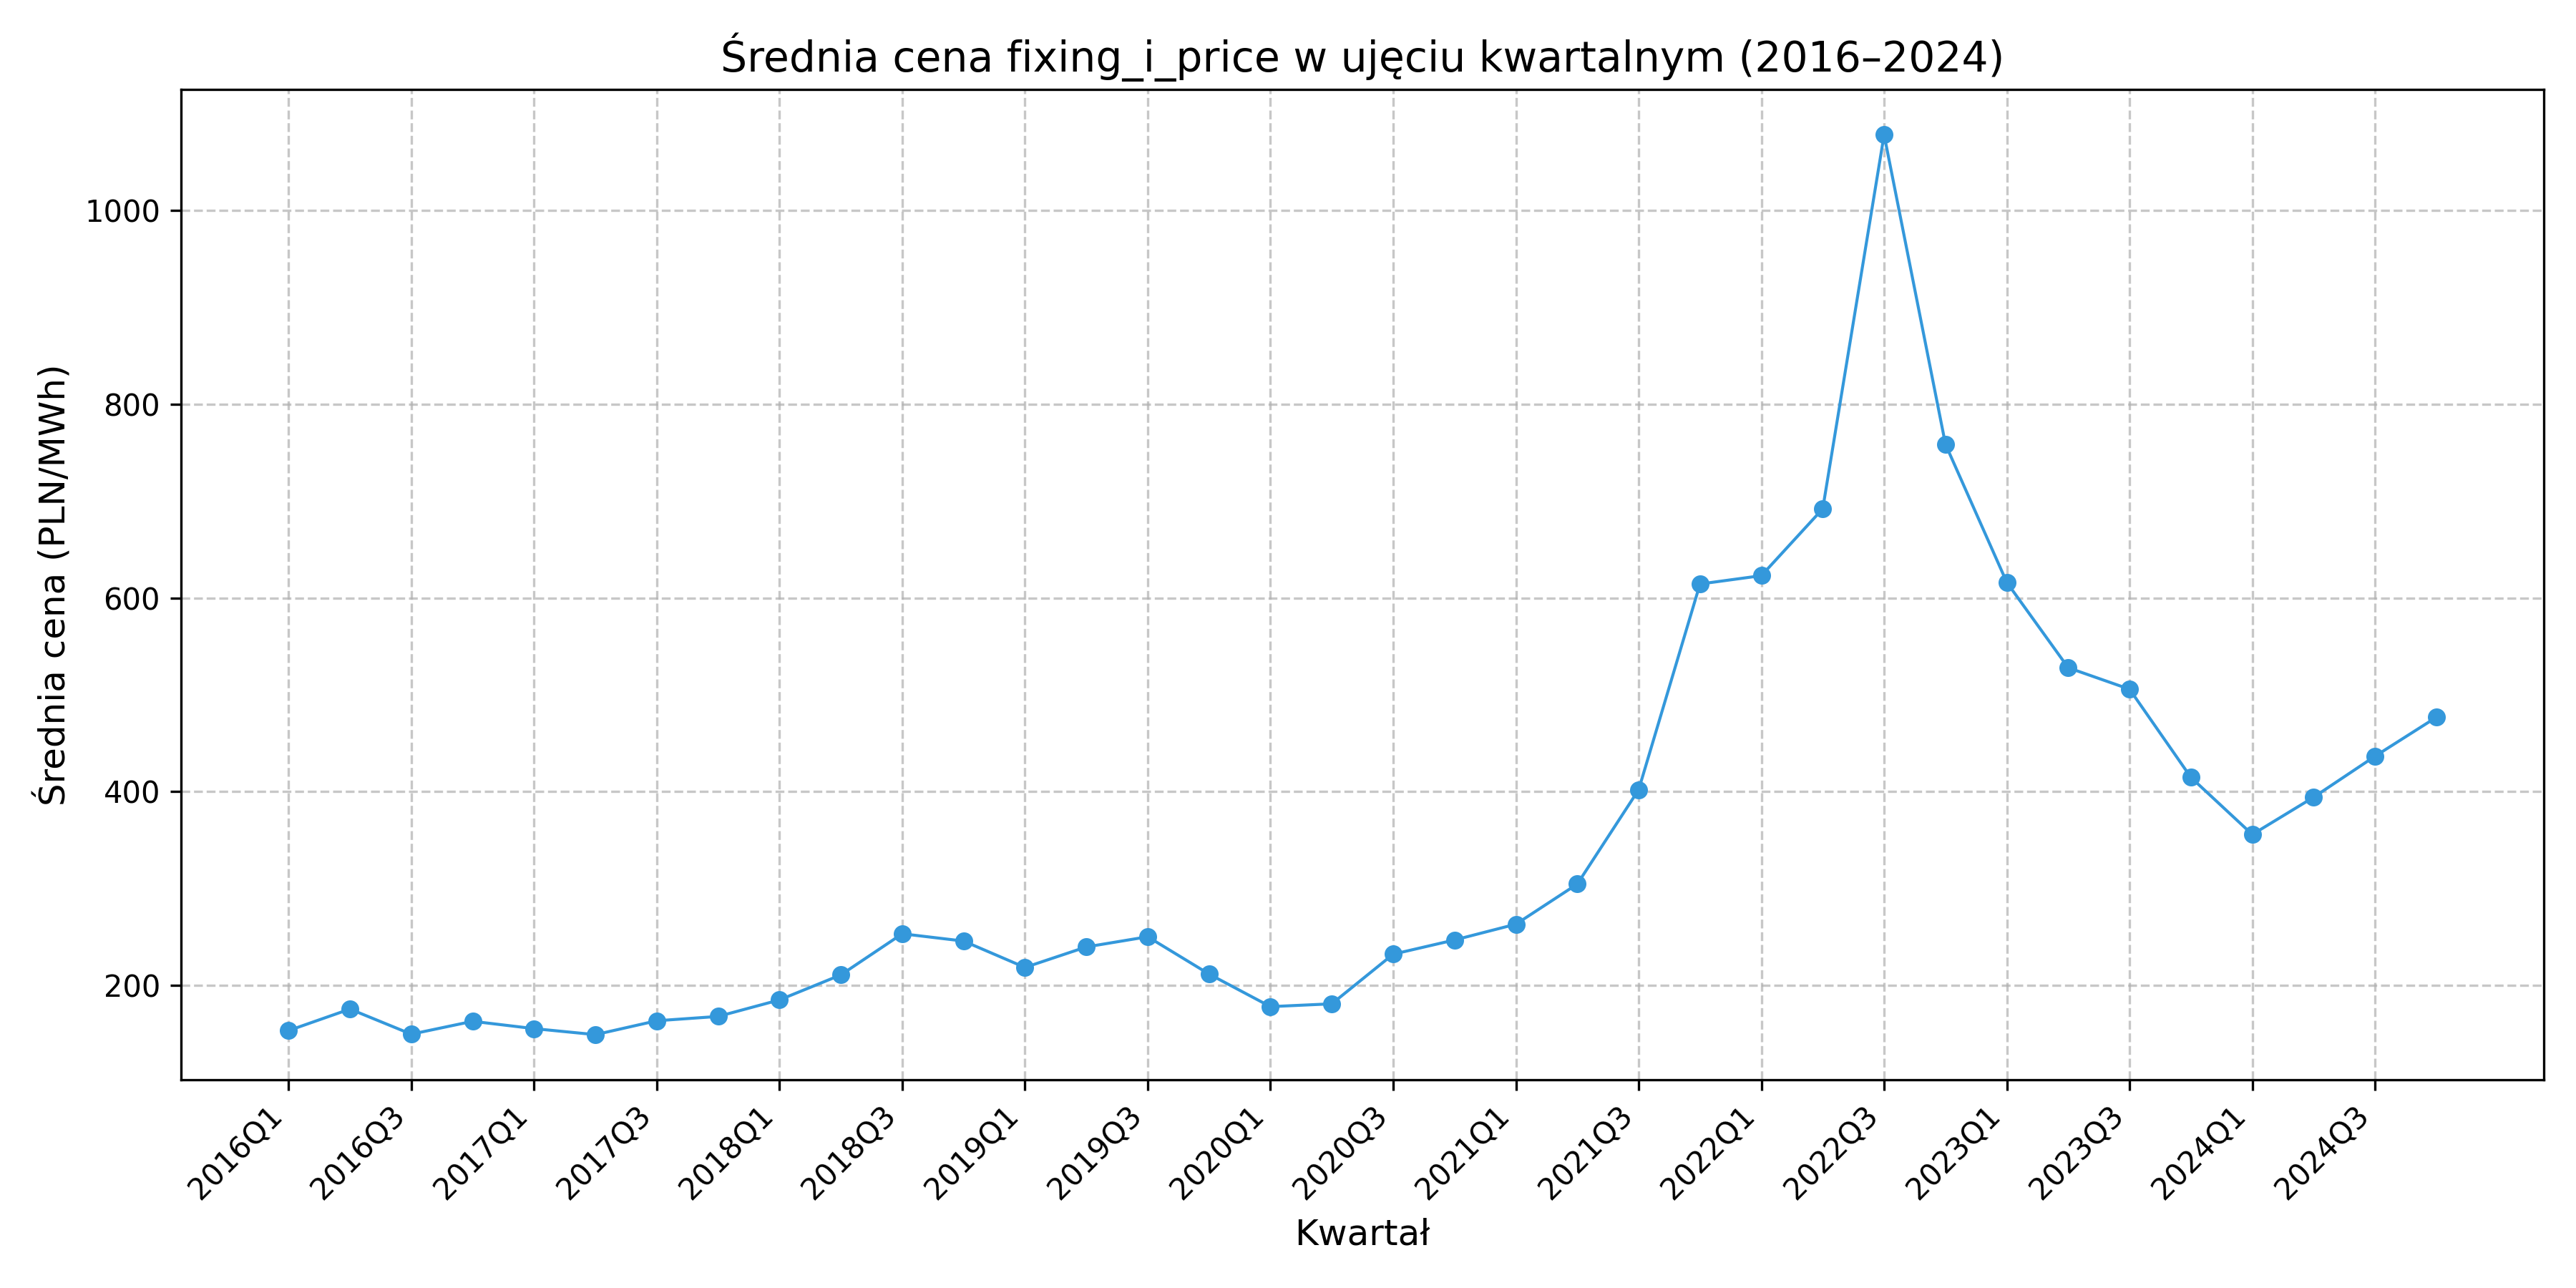
\includegraphics[width=\textwidth]{../plots/quarterly_fixing_i_price.png}
    \caption{Zmienność cen energii elektrycznej na RDN w latach 2016–2024}
    \label{fig:fixing-i-price-trend}
\end{figure}

Widać wyraźne różnice w poziomie cen w różnych okresach: od 2016 do Q4 roku 2020 ceny były stosunkowo stabilne, oscylując w przedziale 100–300 PLN/MWh. Sytuacja zmieniła się w 2020 roku, gdy zaczęły pojawiać się pierwsze skoki cenowe z powodu poważnych obostrzeń z powodu pandemii, a w 2022 roku, w wyniku kryzysu energetycznego wywołanego wojną na Ukrainie i ograniczeniami w dostawach paliw kopalnych, ceny osiągnęły rekordowe poziomy. Pierwszy okres zostanie określony jako okres stabilności cenowej, a drugi jako okres skoków cenowych. Te dwa okresy pokazują, jak niekorzystne sytuacje gospodarcze mogą wpływać na dynamikę cen energii, co ma istotne implikacje dla modelowania i prognozowania.

\begin{figure}
    \centering
    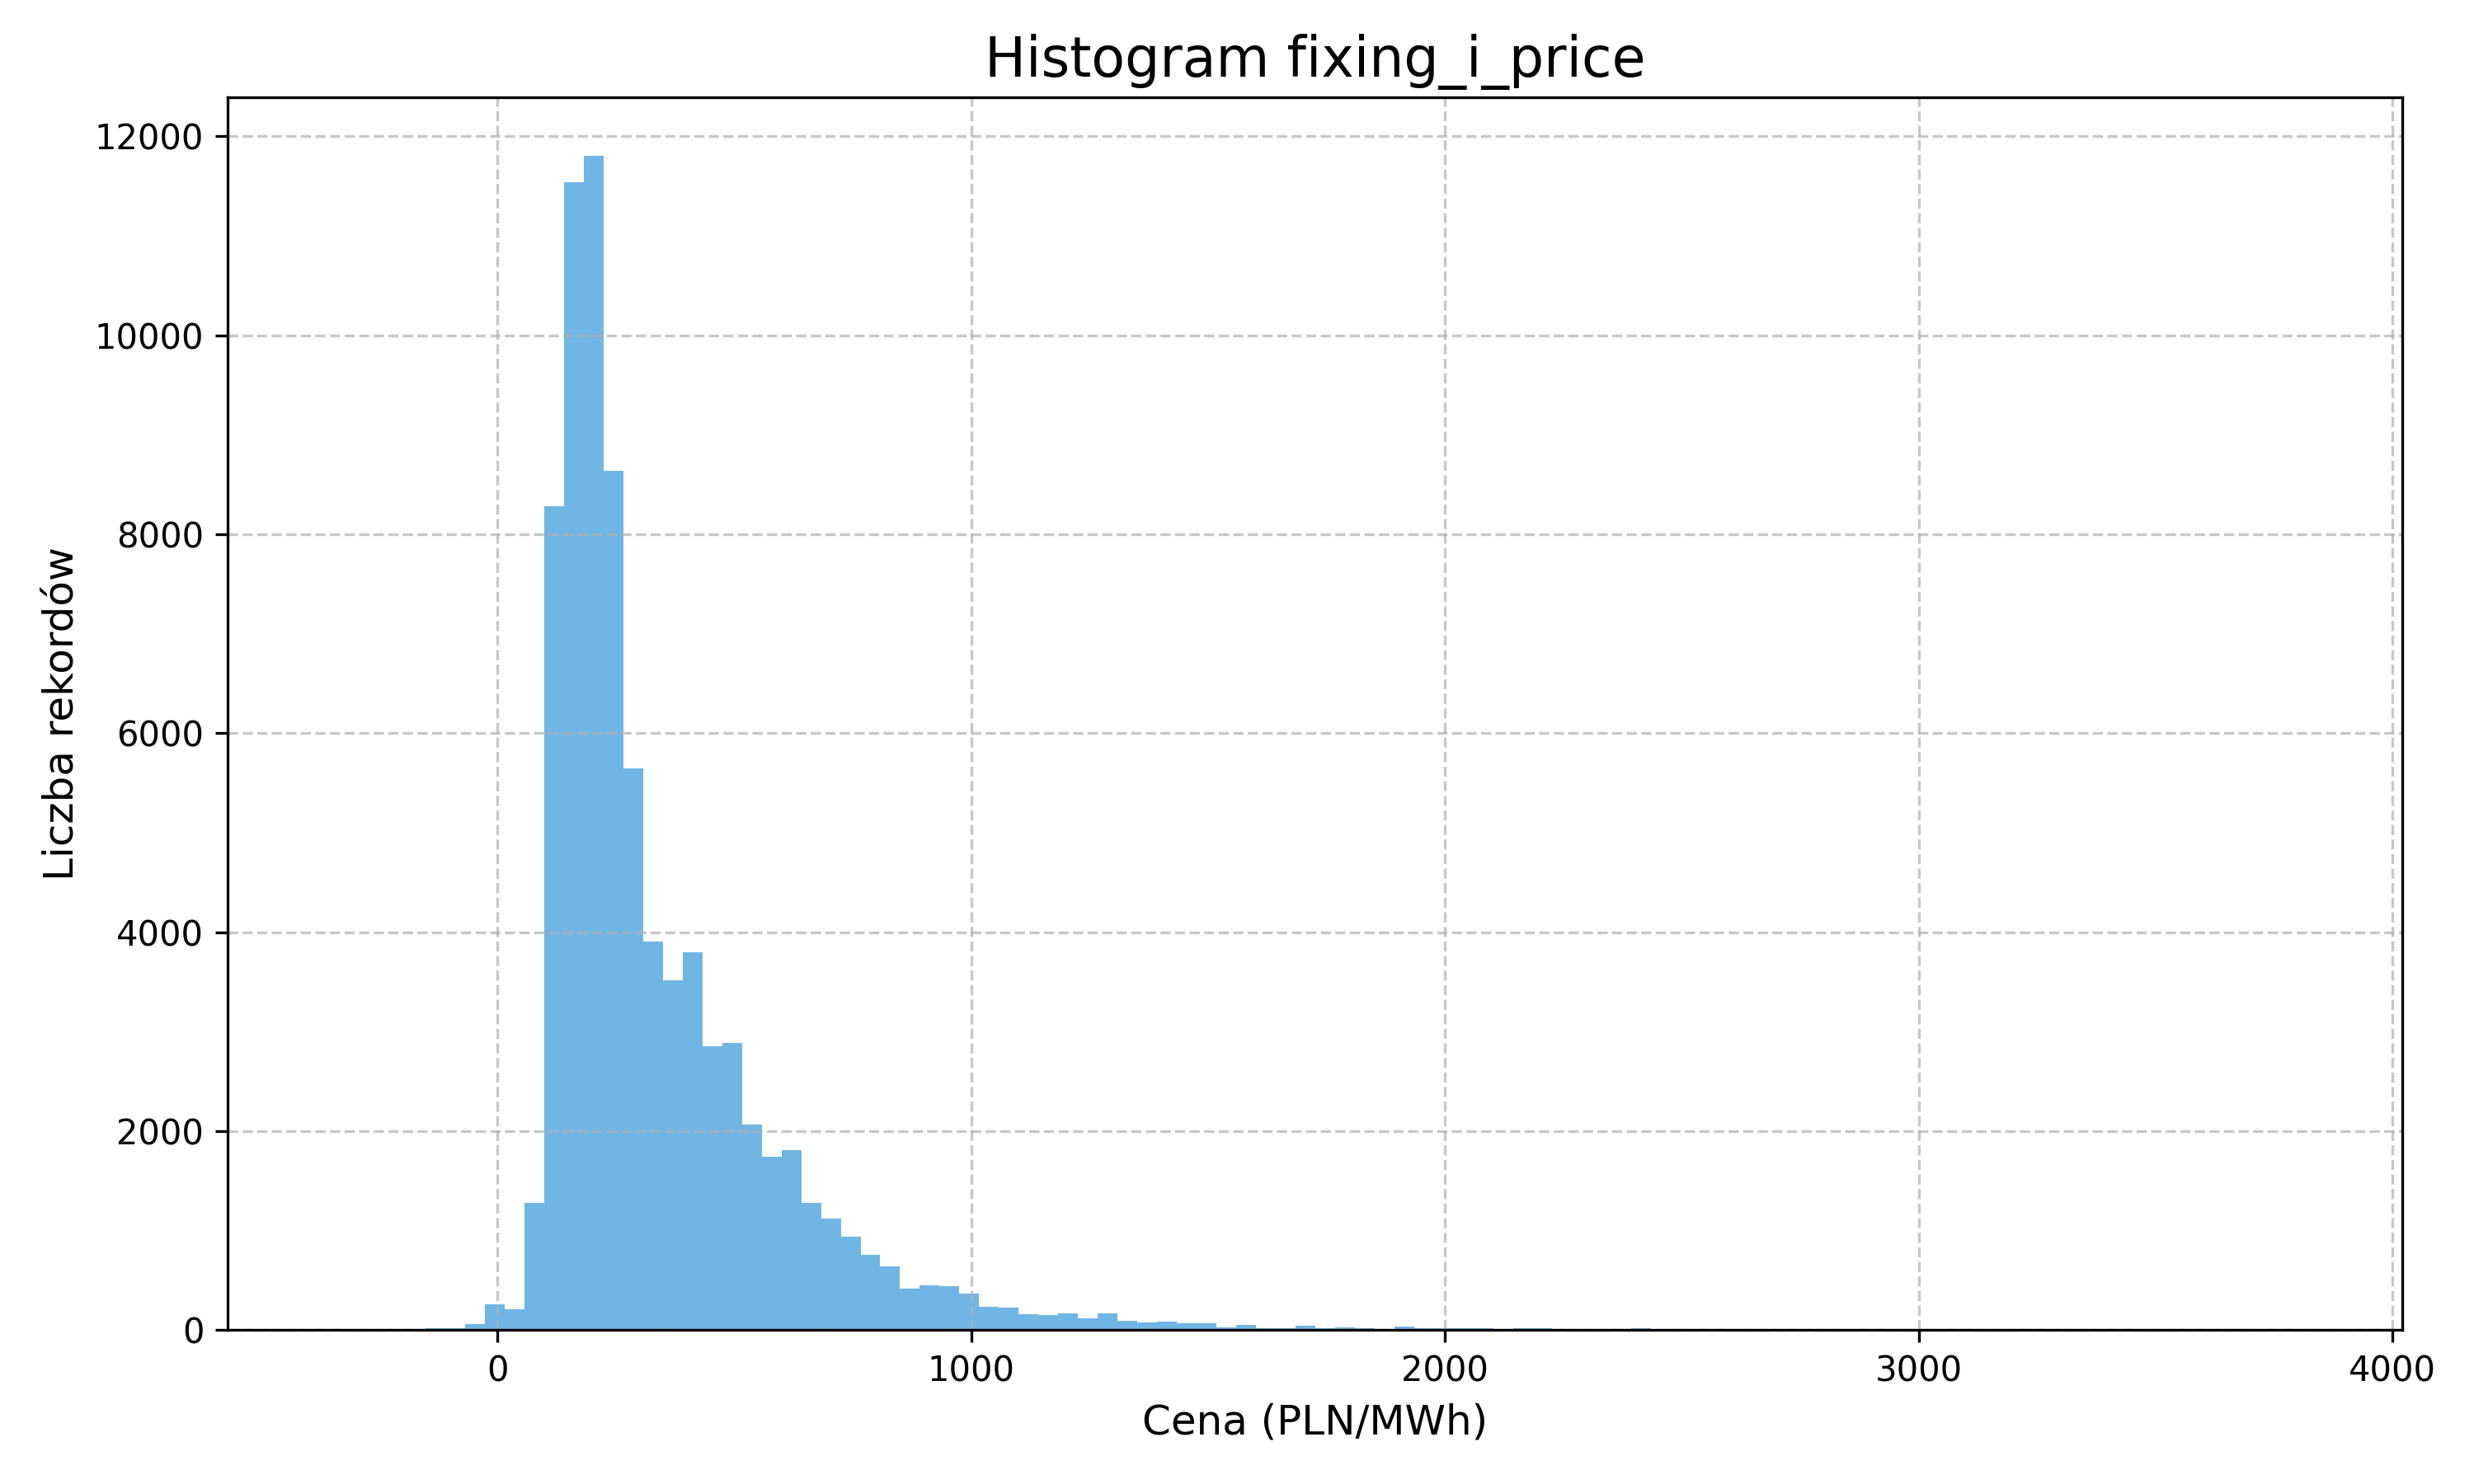
\includegraphics[width=\textwidth]{../plots/fixing_i_price_histogram.png}
    \caption{Histogram rozkładu zmiennej fixing\_i\_price}
    \label{fig:fixing-i-price-histogram}
\end{figure}

Rysunek \ref{fig:fixing-i-price-histogram} przedstawia histogram rozkładu zmiennej \texttt{fixing\_i\_price}. Rozkład jest wyraźnie asymetryczny, z długim prawym ogonem, co odzwierciedla występowanie skoków cenowych, takich jak te w 2022 roku. Ujemne ceny, choć rzadkie (ok. 0,4\% rekordów), są widoczne w lewej części histogramu, co potwierdza specyficzne cechy danych i potrzebę stosowania odpowiednich metod modelowania.

\section{Zbiór zmiennych niezależnych}
Dobór zmiennych niezależnych jest bardzo ważny dla osiągnięcia dobrych wyników badania. W niniejszej pracy wykorzystano różnorodne zmienne niezależne, które można podzielić na kilka kategorii. Obejmują one dane pogodowe, zapotrzebowanie, straty sieciowe, bilanse wymiany transgranicznej, dane o produkcji energii przez poszczególne typy generatorów, ceny paliw kopalnych, emisji CO$_2$ i inne. Wybór tych zmiennych oparty jest na ich potencjalnym wpływie na ceny energii elektrycznej. Poniżej przedstawiono szczegółowy opis każdej z kategorii zmiennych niezależnych, które zostały uwzględnione w analizie.

\subsection{Dane pogodowe}
Pierwotnie zbiór danych miał być zestawiony z danych dostępnych za pomocą oficjalnej strony Instytutu Meteorologii i Gospodarki Wodnej, natomiat dane historyczne z lat 2016-2024 mają ograniczoną rozdzielczość. Zbierane są przez wiele stacji meteorologicznych, które są rozproszone po całym kraju, ale tylko w godzinach 6:00, 12:00 oraz 18:00. Aproksymować dane pogodowe w godzinach nocnych jest zadaniem nie do wykonania, szczególnie w przypadku sezonów zimowych, gdzie temperatura w nocy może drastycznie spadać w ciągu godziny. Z tego powodu jako źródło danych pogodowych wykorzystano stronę open-meteo.com \cite{METEO}. Jest to strona, która zbiera dane z różnych stacji meteorologicznych i udostępnia je w formie API. Dzięki temu można pobrać dane pogodowe dla dowolnego okresu czasu i lokalizacji.

Dane pogodowe zostały pobrane dla czterech lokalizacji w Polsce: Warszawy (WAW), Koszalina (KSZ), Krakowa (KRK) i Babimost (BAB), a następnie dopasowane do godzinowego formatu danych RDN, co pozwoliło na ich integrację z pozostałymi zmiennymi. Wybór miast został podyktowany ich zróżnicowaniem geograficznym i klimatycznym, co pozwala uwzględnić regionalne różnice w warunkach pogodowych wpływających na produkcję i zapotrzebowanie na energię. Warszawa, jako stolica i największe miasto Polski, reprezentuje centralny region kraju o wysokim zapotrzebowaniu na energię, szczególnie w okresach zimowych i letnich. Koszalin, położony na Pomorzu, jest kluczowy ze względu na bliskość farm wiatrowych na Morzu Bałtyckim, co czyni go istotnym punktem dla analizy produkcji energii wiatrowej. Kraków, znajdujący się w południowej Polsce, charakteryzuje się większym udziałem energii słonecznej w miksie energetycznym, a także wysokim zapotrzebowaniem na energię w sezonie grzewczym z powodu zanieczyszczenia powietrza i częstego stosowania ogrzewania elektrycznego. Babimost, zlokalizowany w zachodniej Polsce, jest istotny ze względu na swoje położenie w pobliżu granicy z Niemcami.

Parametry pogodowe zostały wybrane z uwzględnieniem ich bezpośredniego wpływu na rynek energii. Temperatura jest kluczowym czynnikiem, ponieważ wpływa na zapotrzebowanie na energię – niskie temperatury zwiększają zużycie energii na ogrzewanie, natomiast wysokie temperatury latem podnoszą zapotrzebowanie na klimatyzację. Prędkość wiatru mierzona na wysokości 100 metrów nad powierzchnią ziemi została wybrana, ponieważ jest to przeciętna wysokość dla turbin wiatrowych w Polsce, co pozwala dokładniej oszacować potencjalną produkcję energii z farm wiatrowych. Promieniowanie słoneczne jest istotne dla produkcji energii z paneli fotowoltaicznych. Zachmurzenie zostało uwzględnione, ponieważ wysoki poziom zachmurzenia zmniejsza efektywność paneli słonecznych, co może zwiększać ceny energii poprzez ograniczenie podaży z OZE. Wybór tych parametrów pozwala na kompleksową analizę wpływu pogody na ceny energii na RDN.

Poniżej przedstawię wykresy dla każdego z parametrów pogodowych, które zostały uwzględnione w analizie. Wykresy przedstawiają zmienność danych pogodowych w czasie. Zachmurzenie jest wyrażone w oktantach (0-8), gdzie 0 oznacza brak zachmurzenia, a 8 oznacza całkowite zachmurzenie.

\begin{figure}[H]
    \centering
    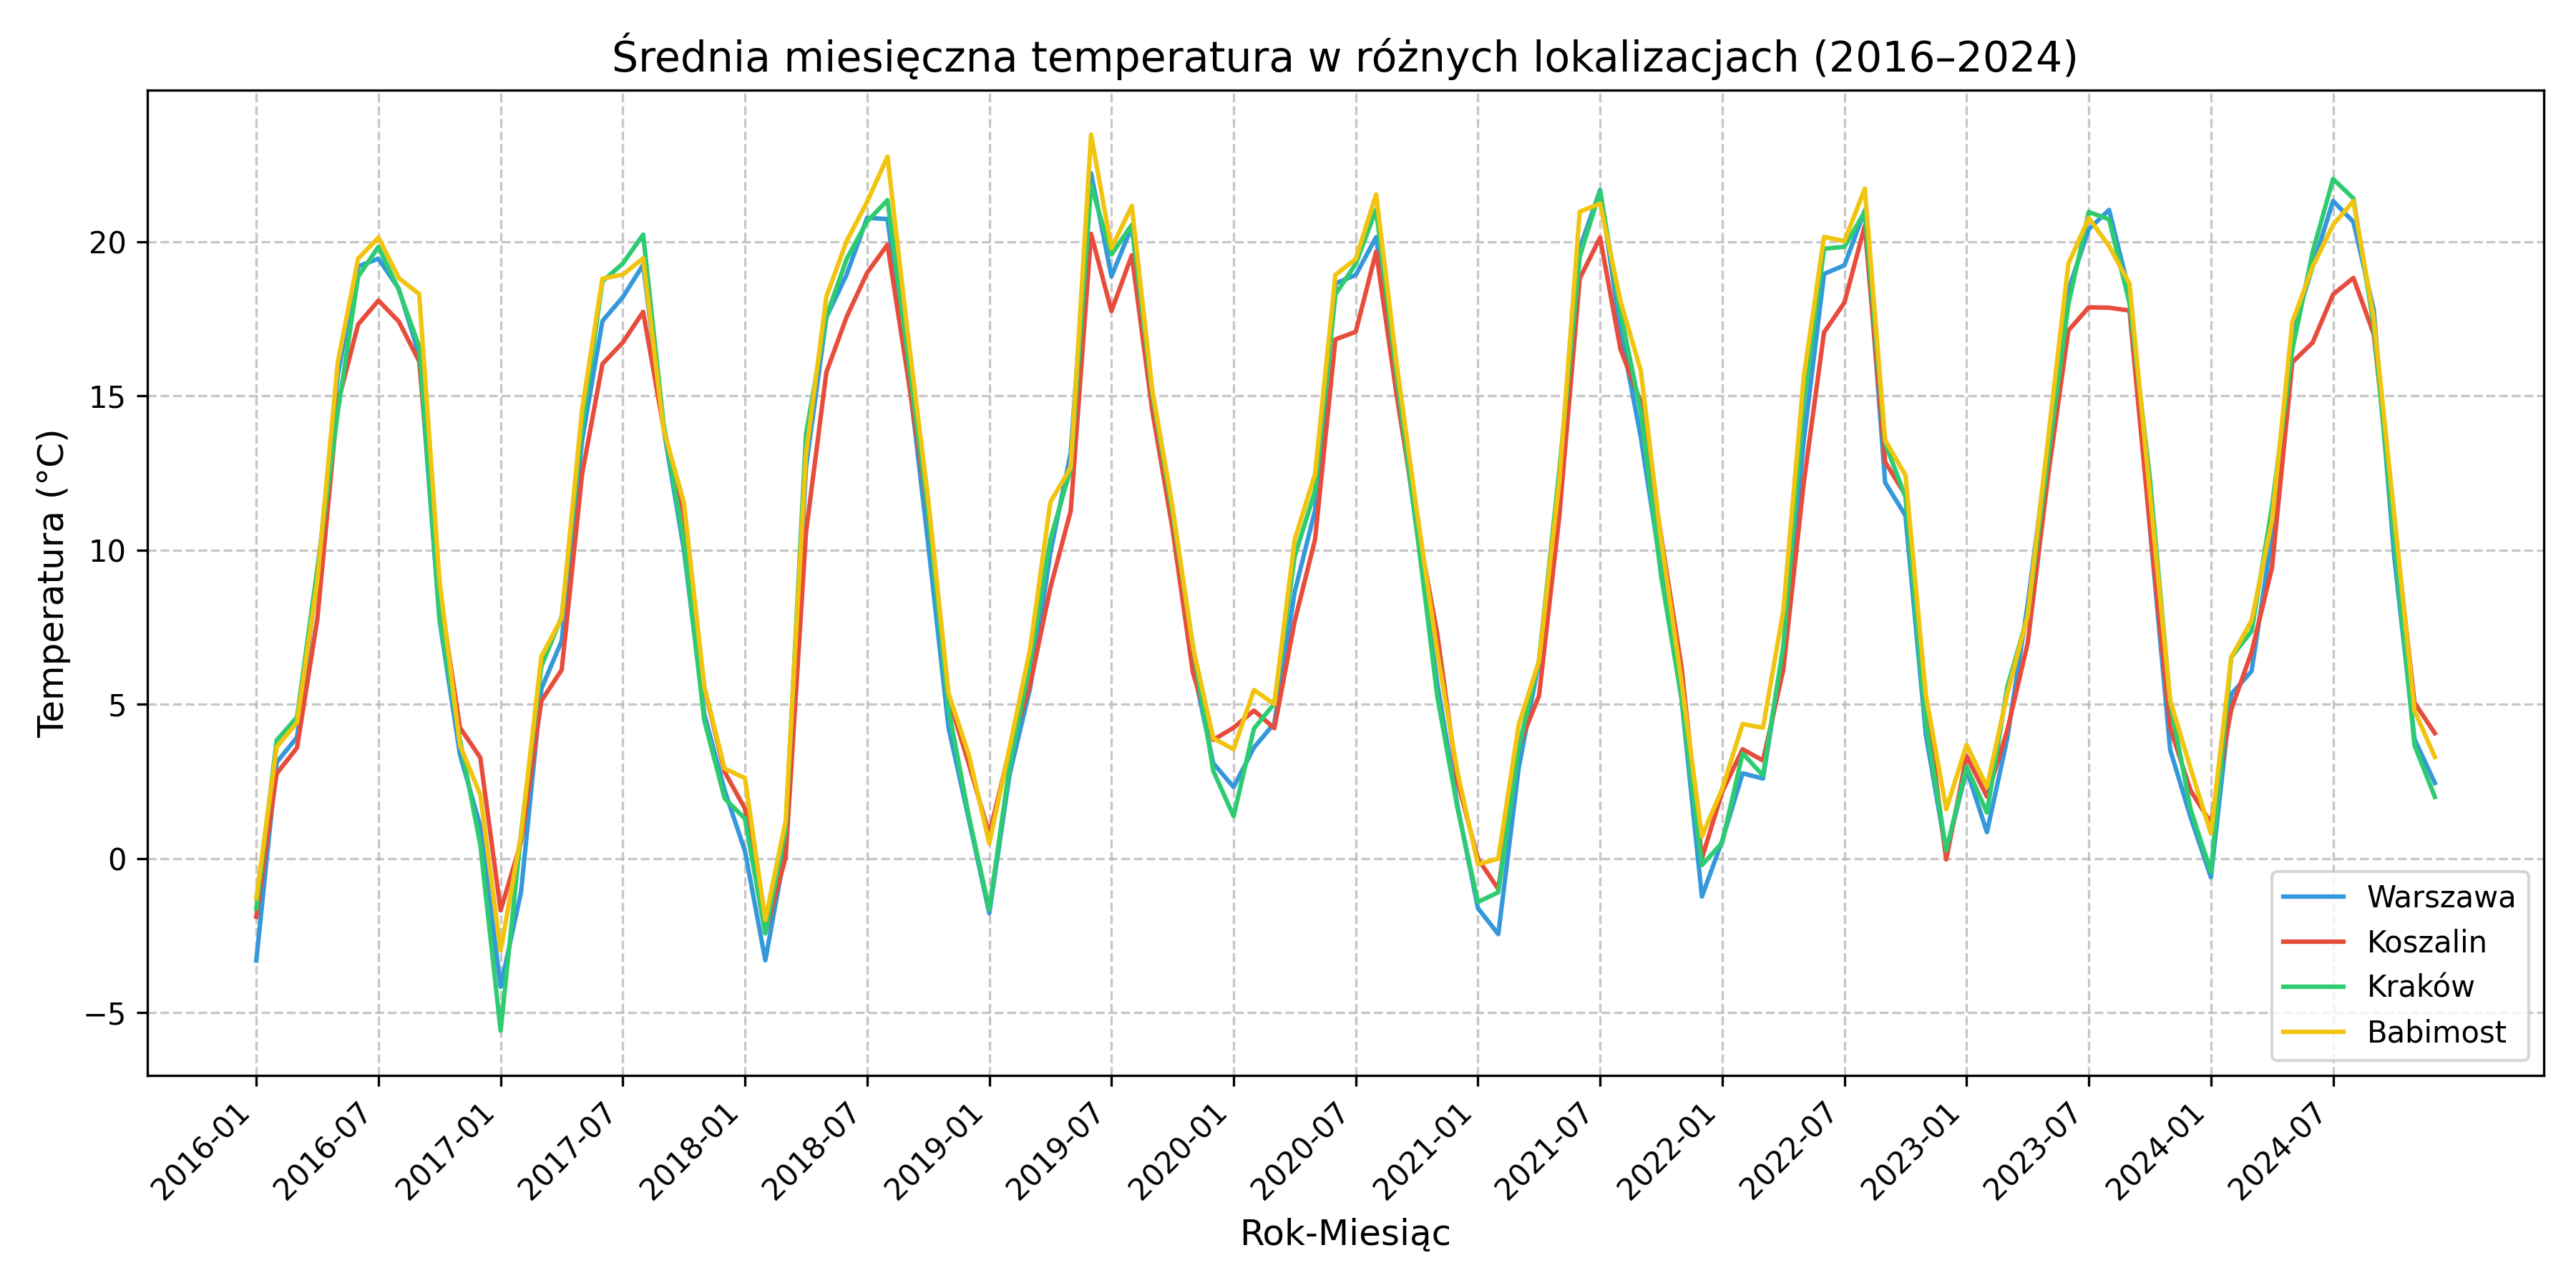
\includegraphics[width=\textwidth]{../plots/weather/temp_time_series_full.png}
    \caption{Zmienność temperatury w czasie (2016–2024)}
    \label{fig:temp-time-series-full}
\end{figure}

\begin{figure}[H]
    \centering
    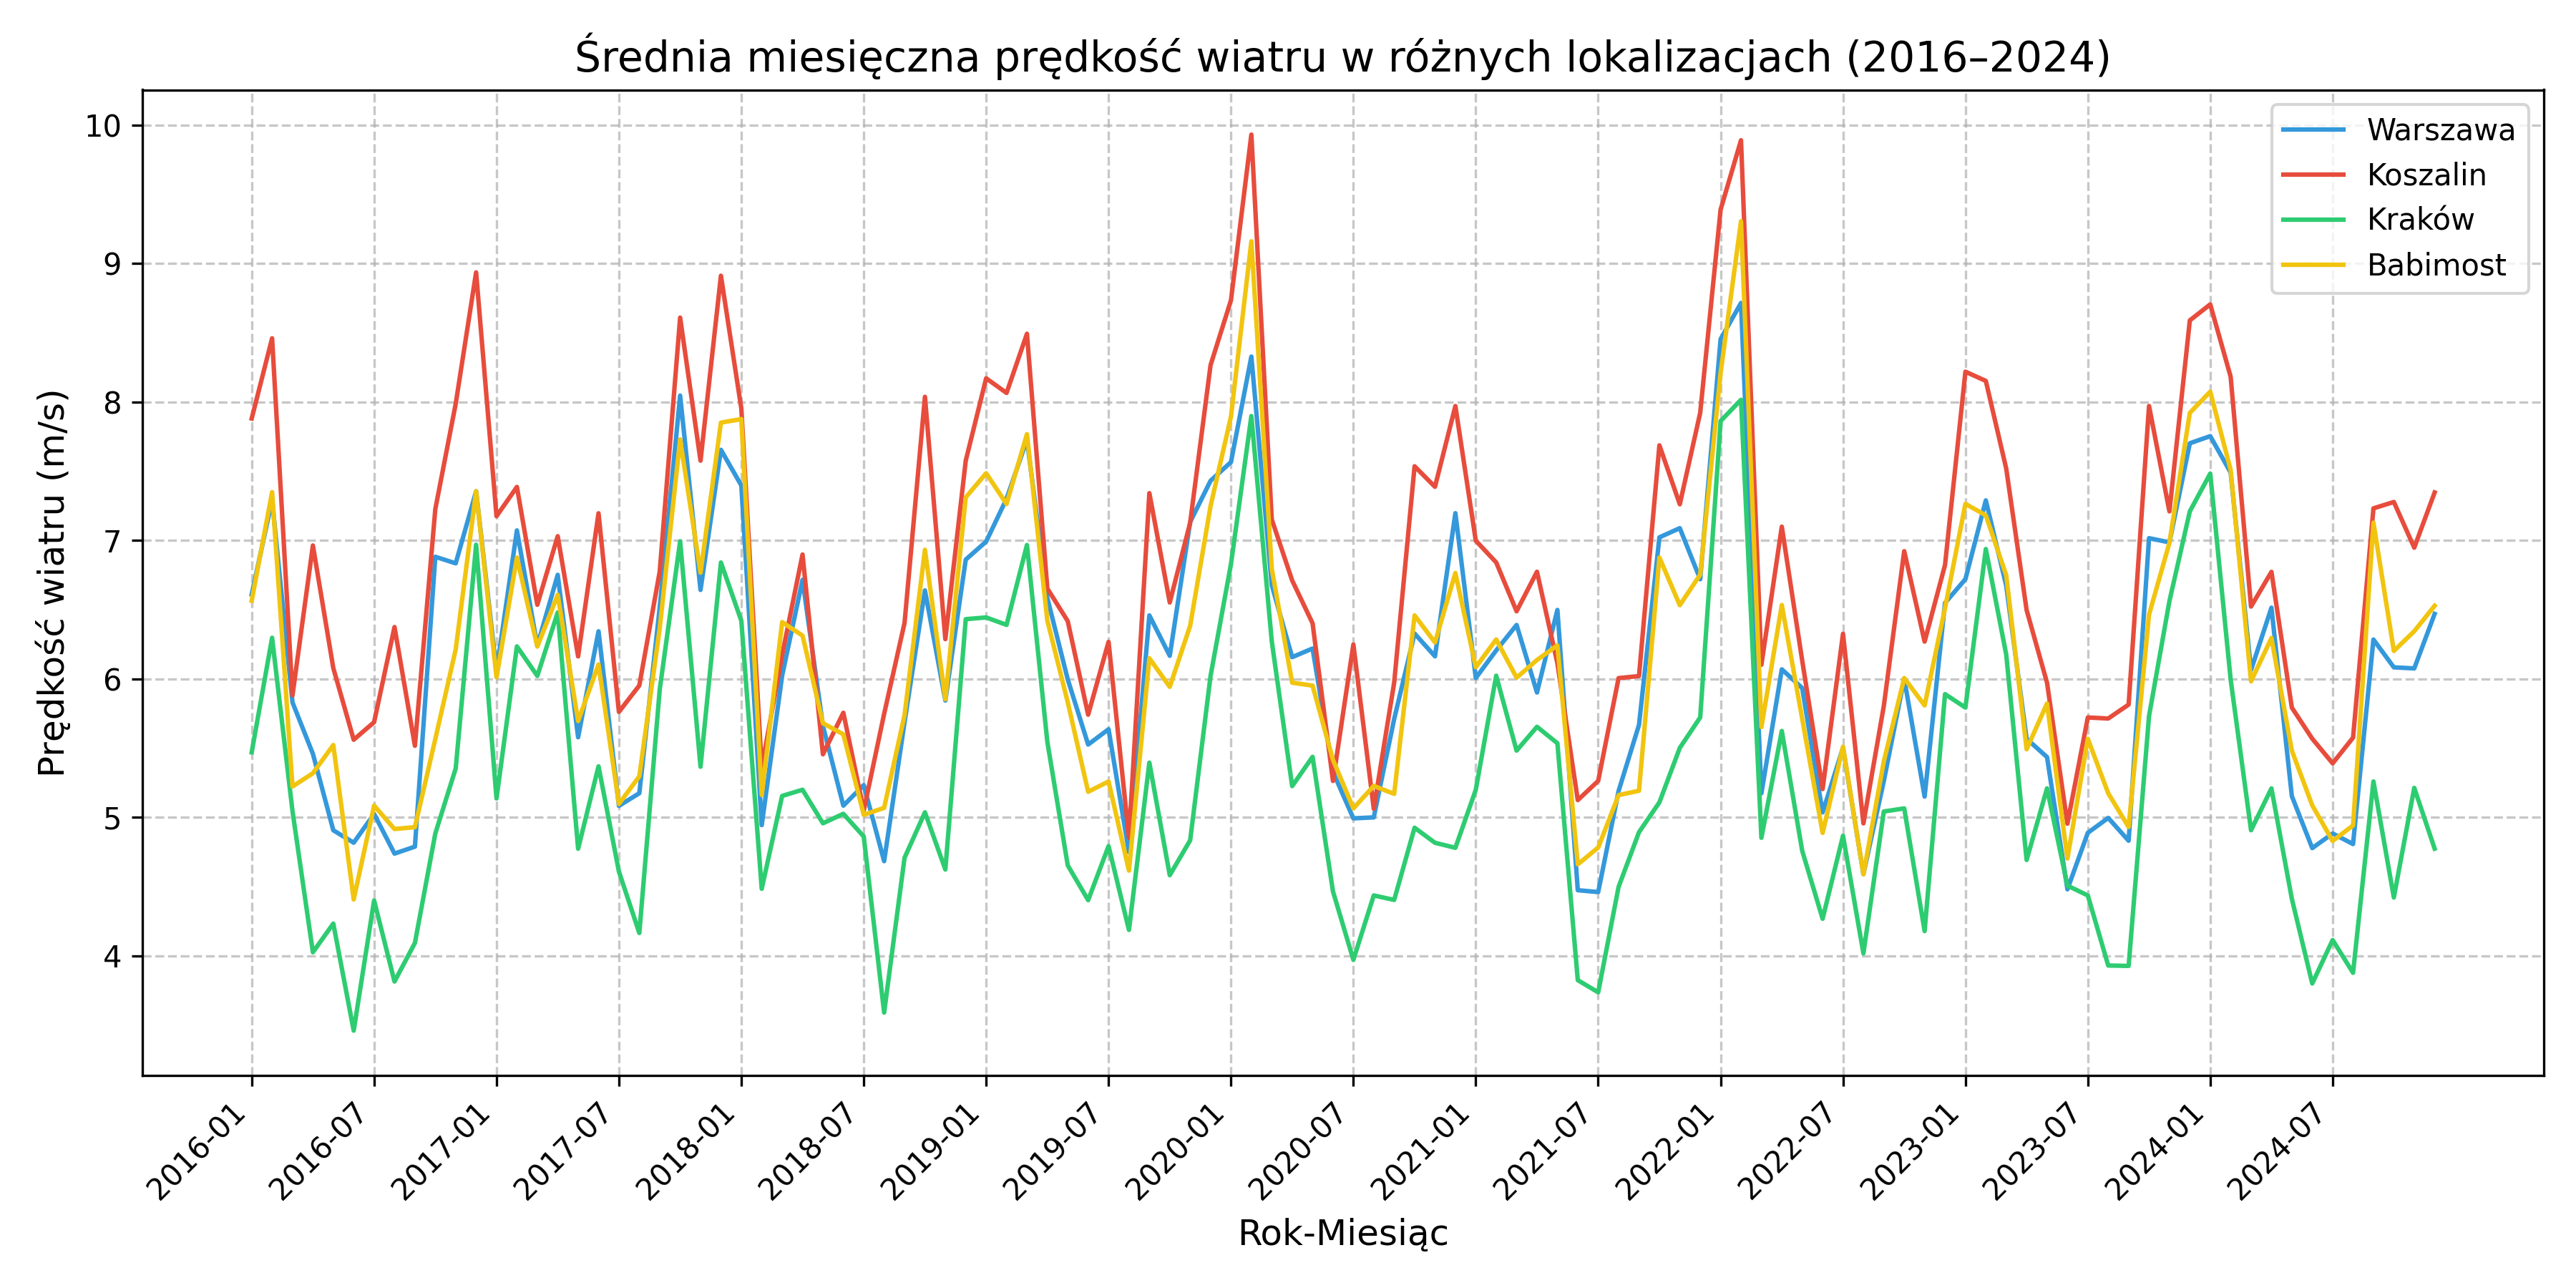
\includegraphics[width=\textwidth]{../plots/weather/wind_speed_time_series_full.png}
    \caption{Zmienność prędkości wiatru w czasie (2016–2024)}
    \label{fig:wind-speed-time-series-full}
\end{figure}

\begin{figure}[H]
    \centering
    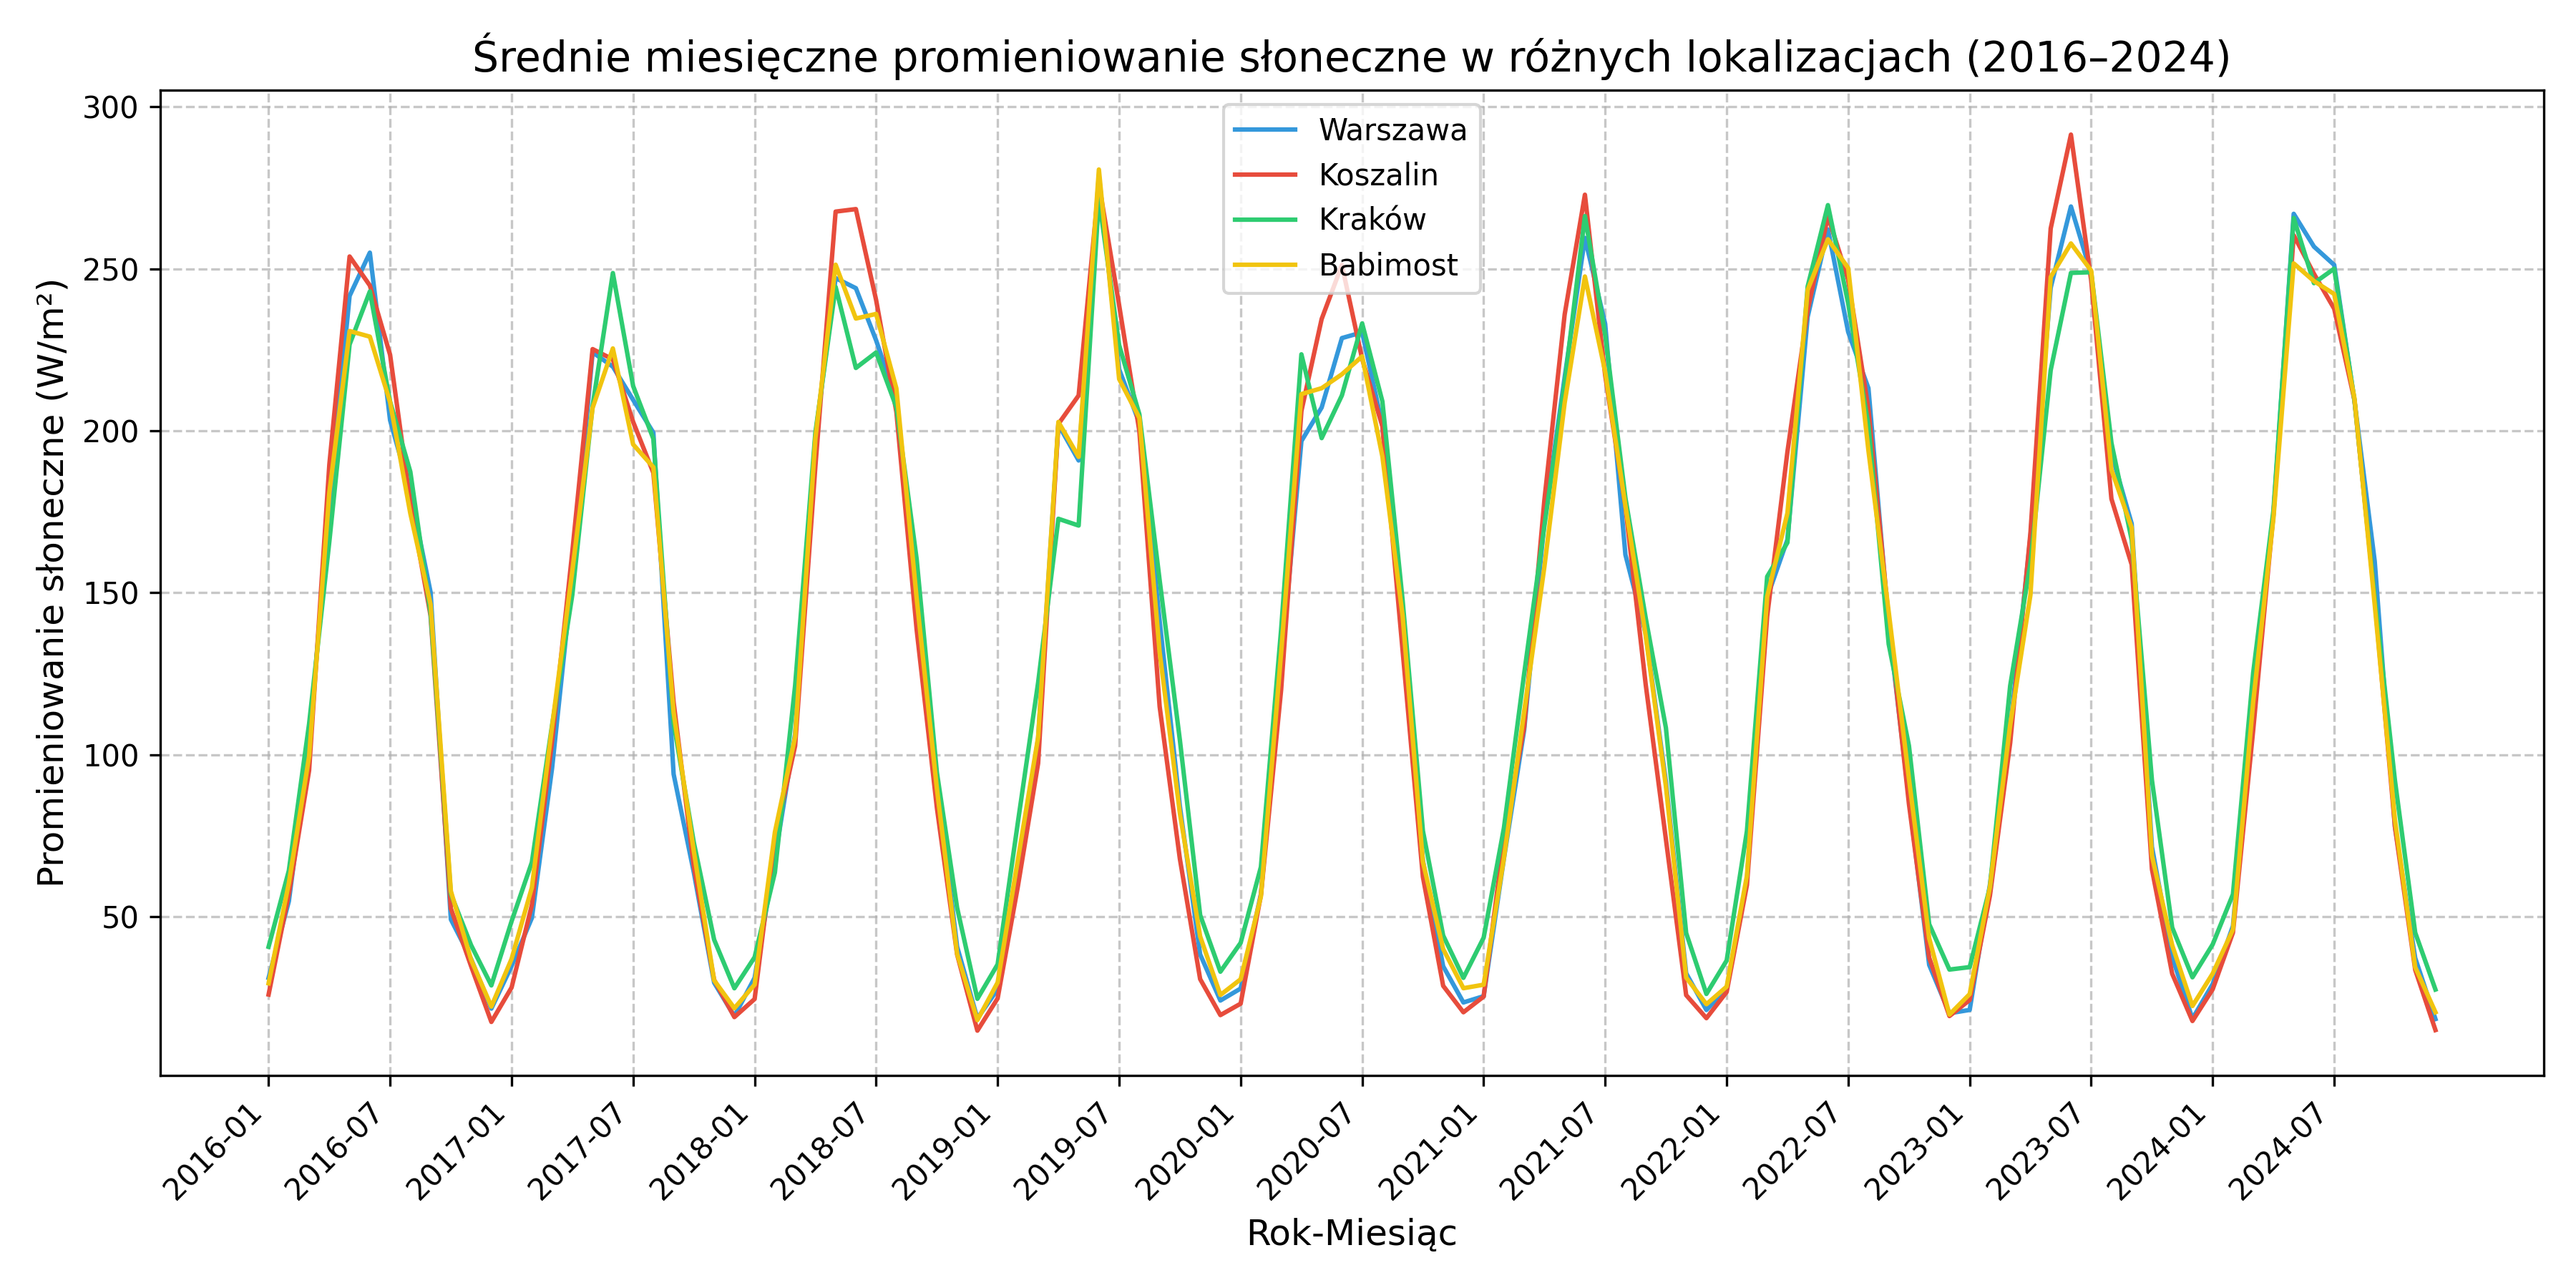
\includegraphics[width=\textwidth]{../plots/weather/solar_radiation_time_series_full.png}
    \caption{Zmienność promieniowania słonecznego w czasie (2016–2024)}
    \label{fig:solar-radiation-time-series-full}
\end{figure}

\begin{figure}[H]
    \centering
    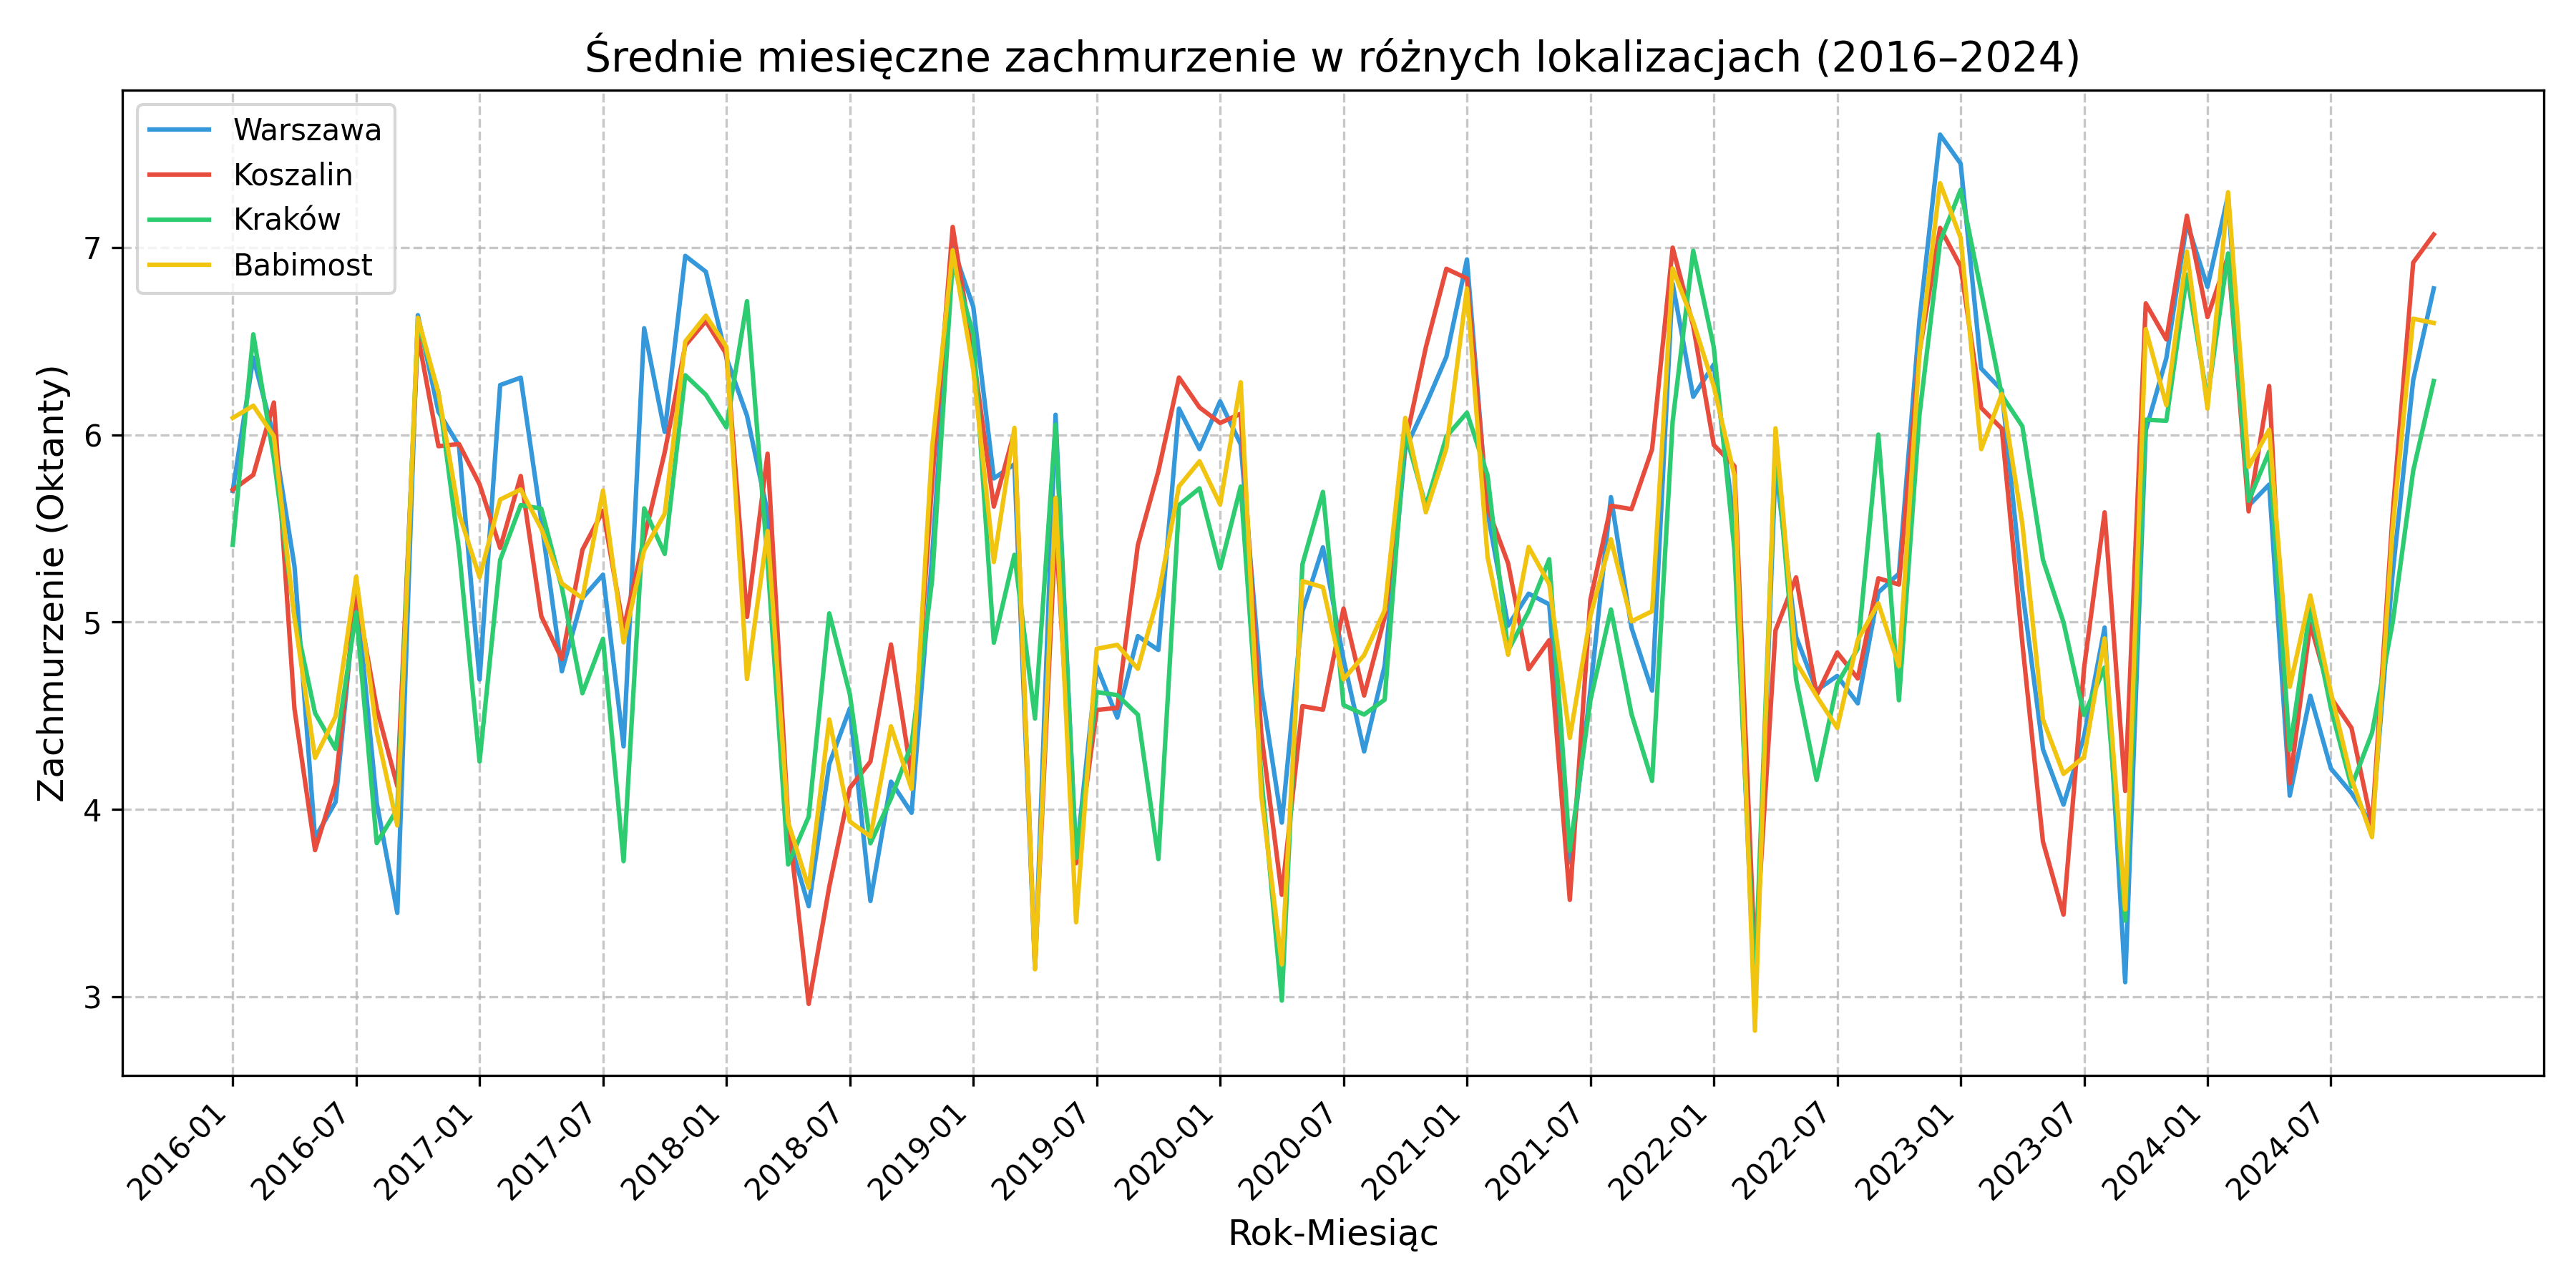
\includegraphics[width=\textwidth]{../plots/weather/cloud_cover_time_series_full.png}
    \caption{Zmienność zachmurzenia w czasie (2016–2024)}
    \label{fig:cloud-cover-time-series-full}
\end{figure}

Każdy z wykresów przedstawia zmienność danego parametru pogodowego w wybranych lokalizacjach w przeciągu okresu badawczego. Wyraźnie widać sezonowe wahania parametrów pogodowych, co jest typowe dla klimatu Polski. Temperatura i promieniowanie słoneczne mają wyraźnie większe wartości w sezonach letnich, prędkość wiatru w sezonach zimowych, a zachmurzenie ma bardziej zróżnicowany charakter.

Chciałbym również przybliżyć wykresy i potwierdzić efekt sezonowości na przykładzie 2022 roku. 

\begin{figure}[H]
    \centering
    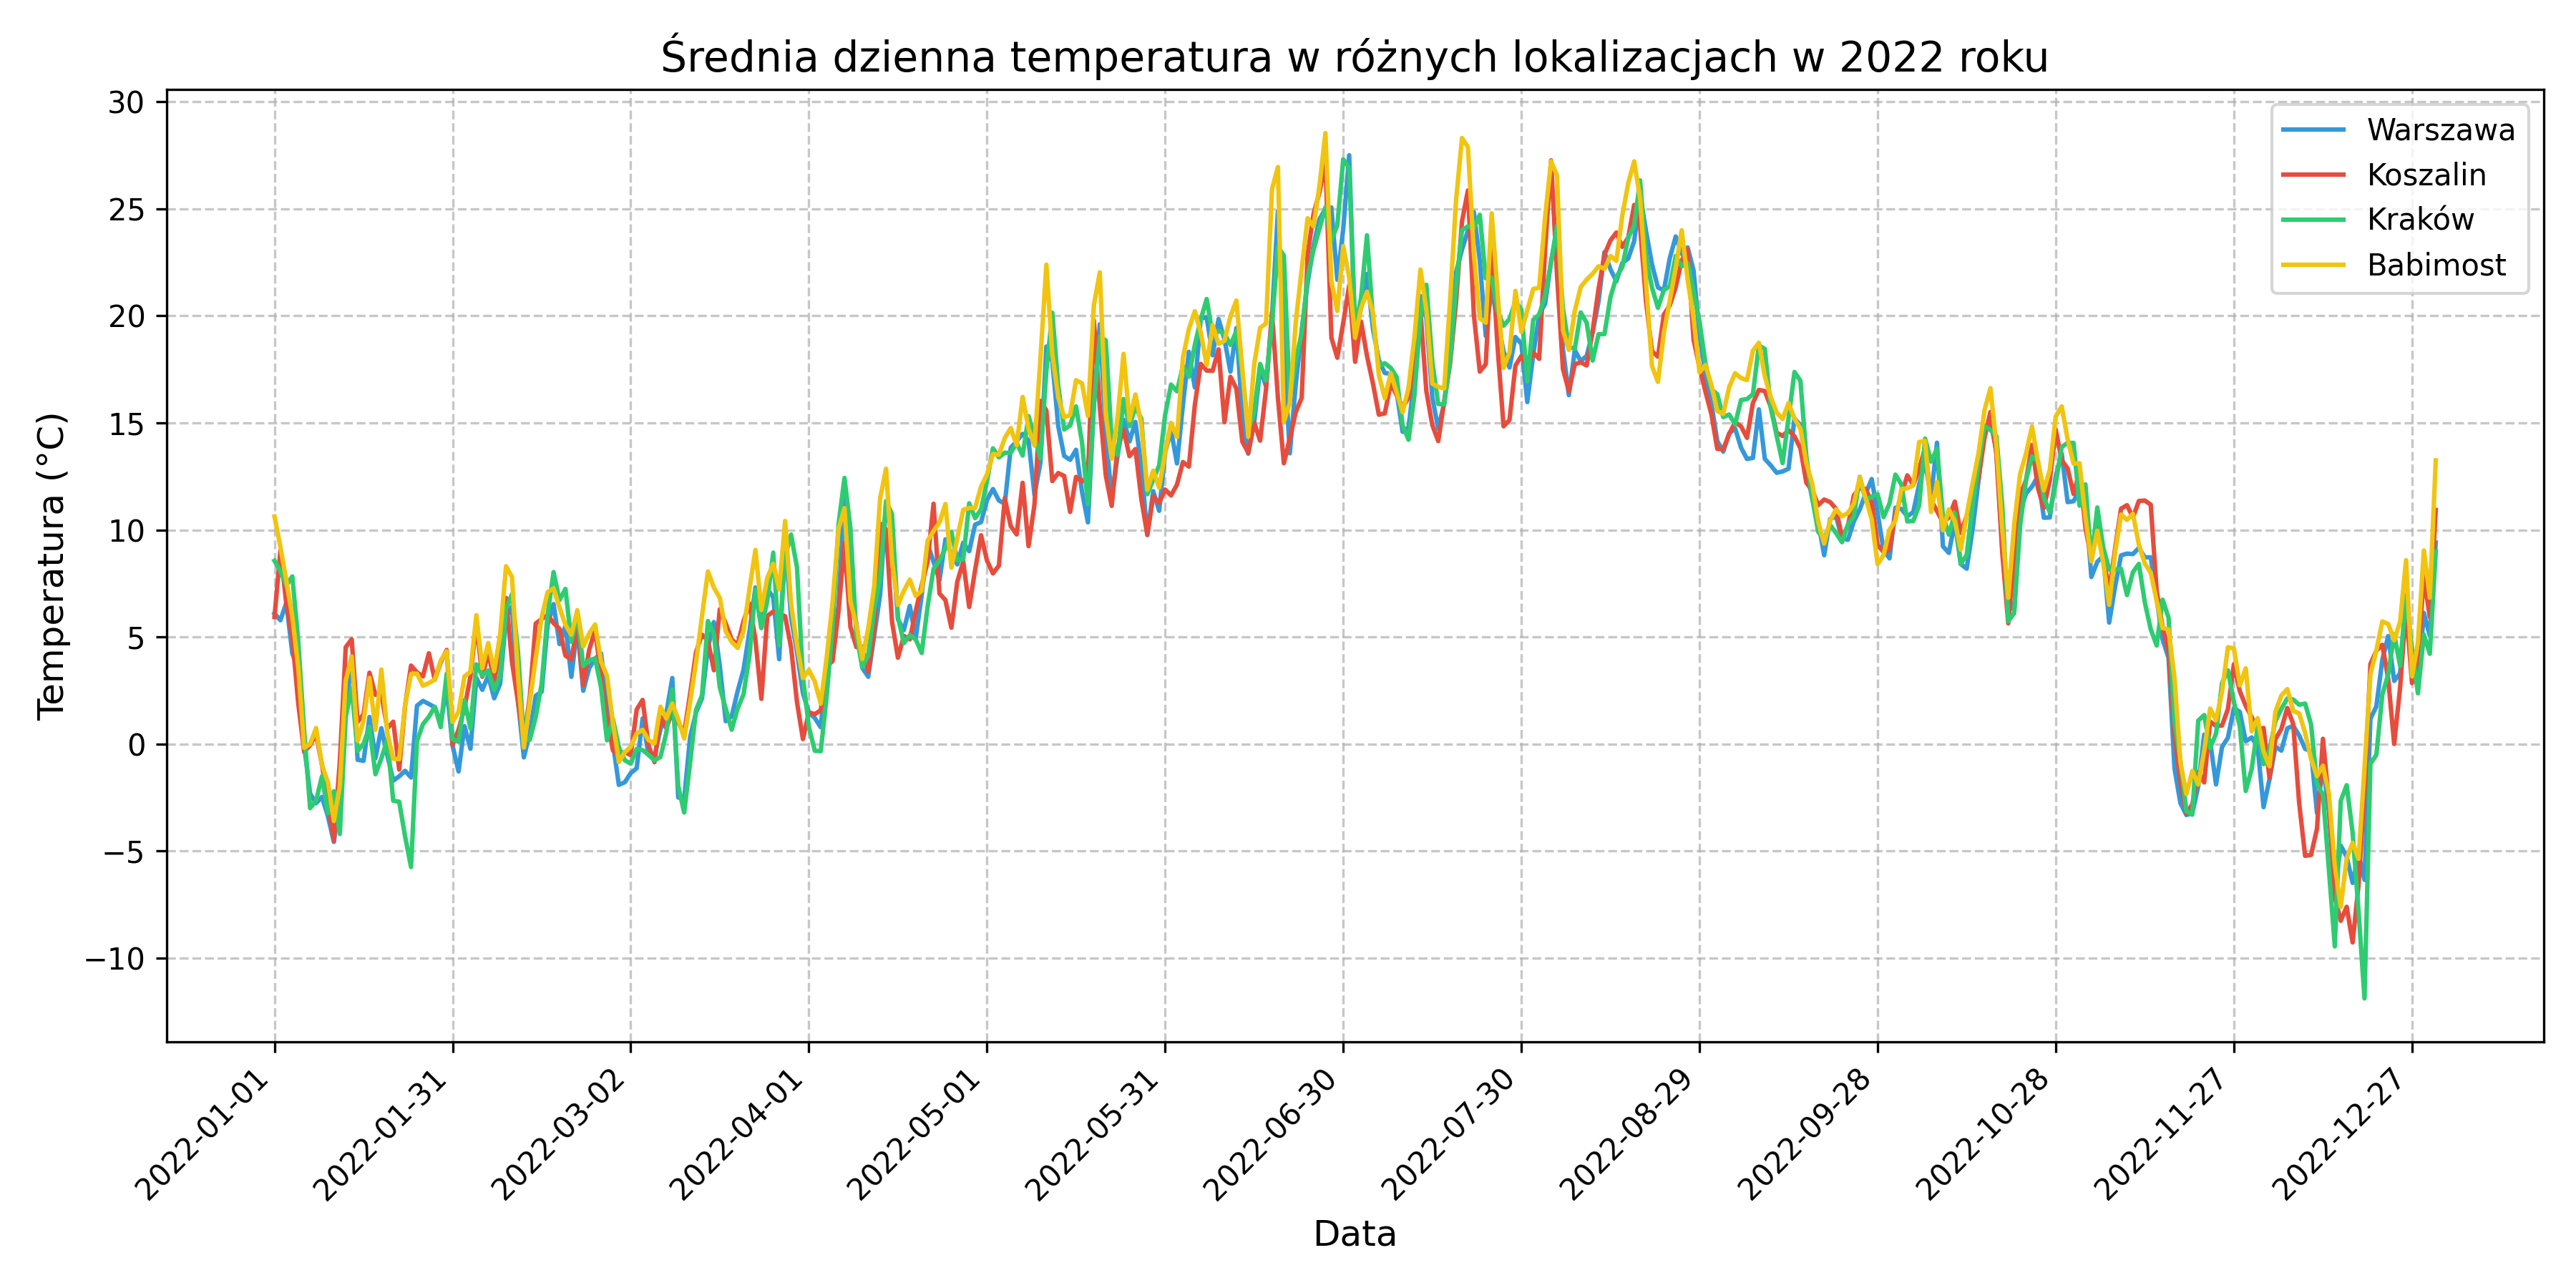
\includegraphics[width=\textwidth]{../plots/weather/temp_time_series_2022.png}
    \caption{Zmienność temperatury w czasie (2022)}
    \label{fig:temp-time-series-2022}
\end{figure}

\begin{figure}[H]
    \centering
    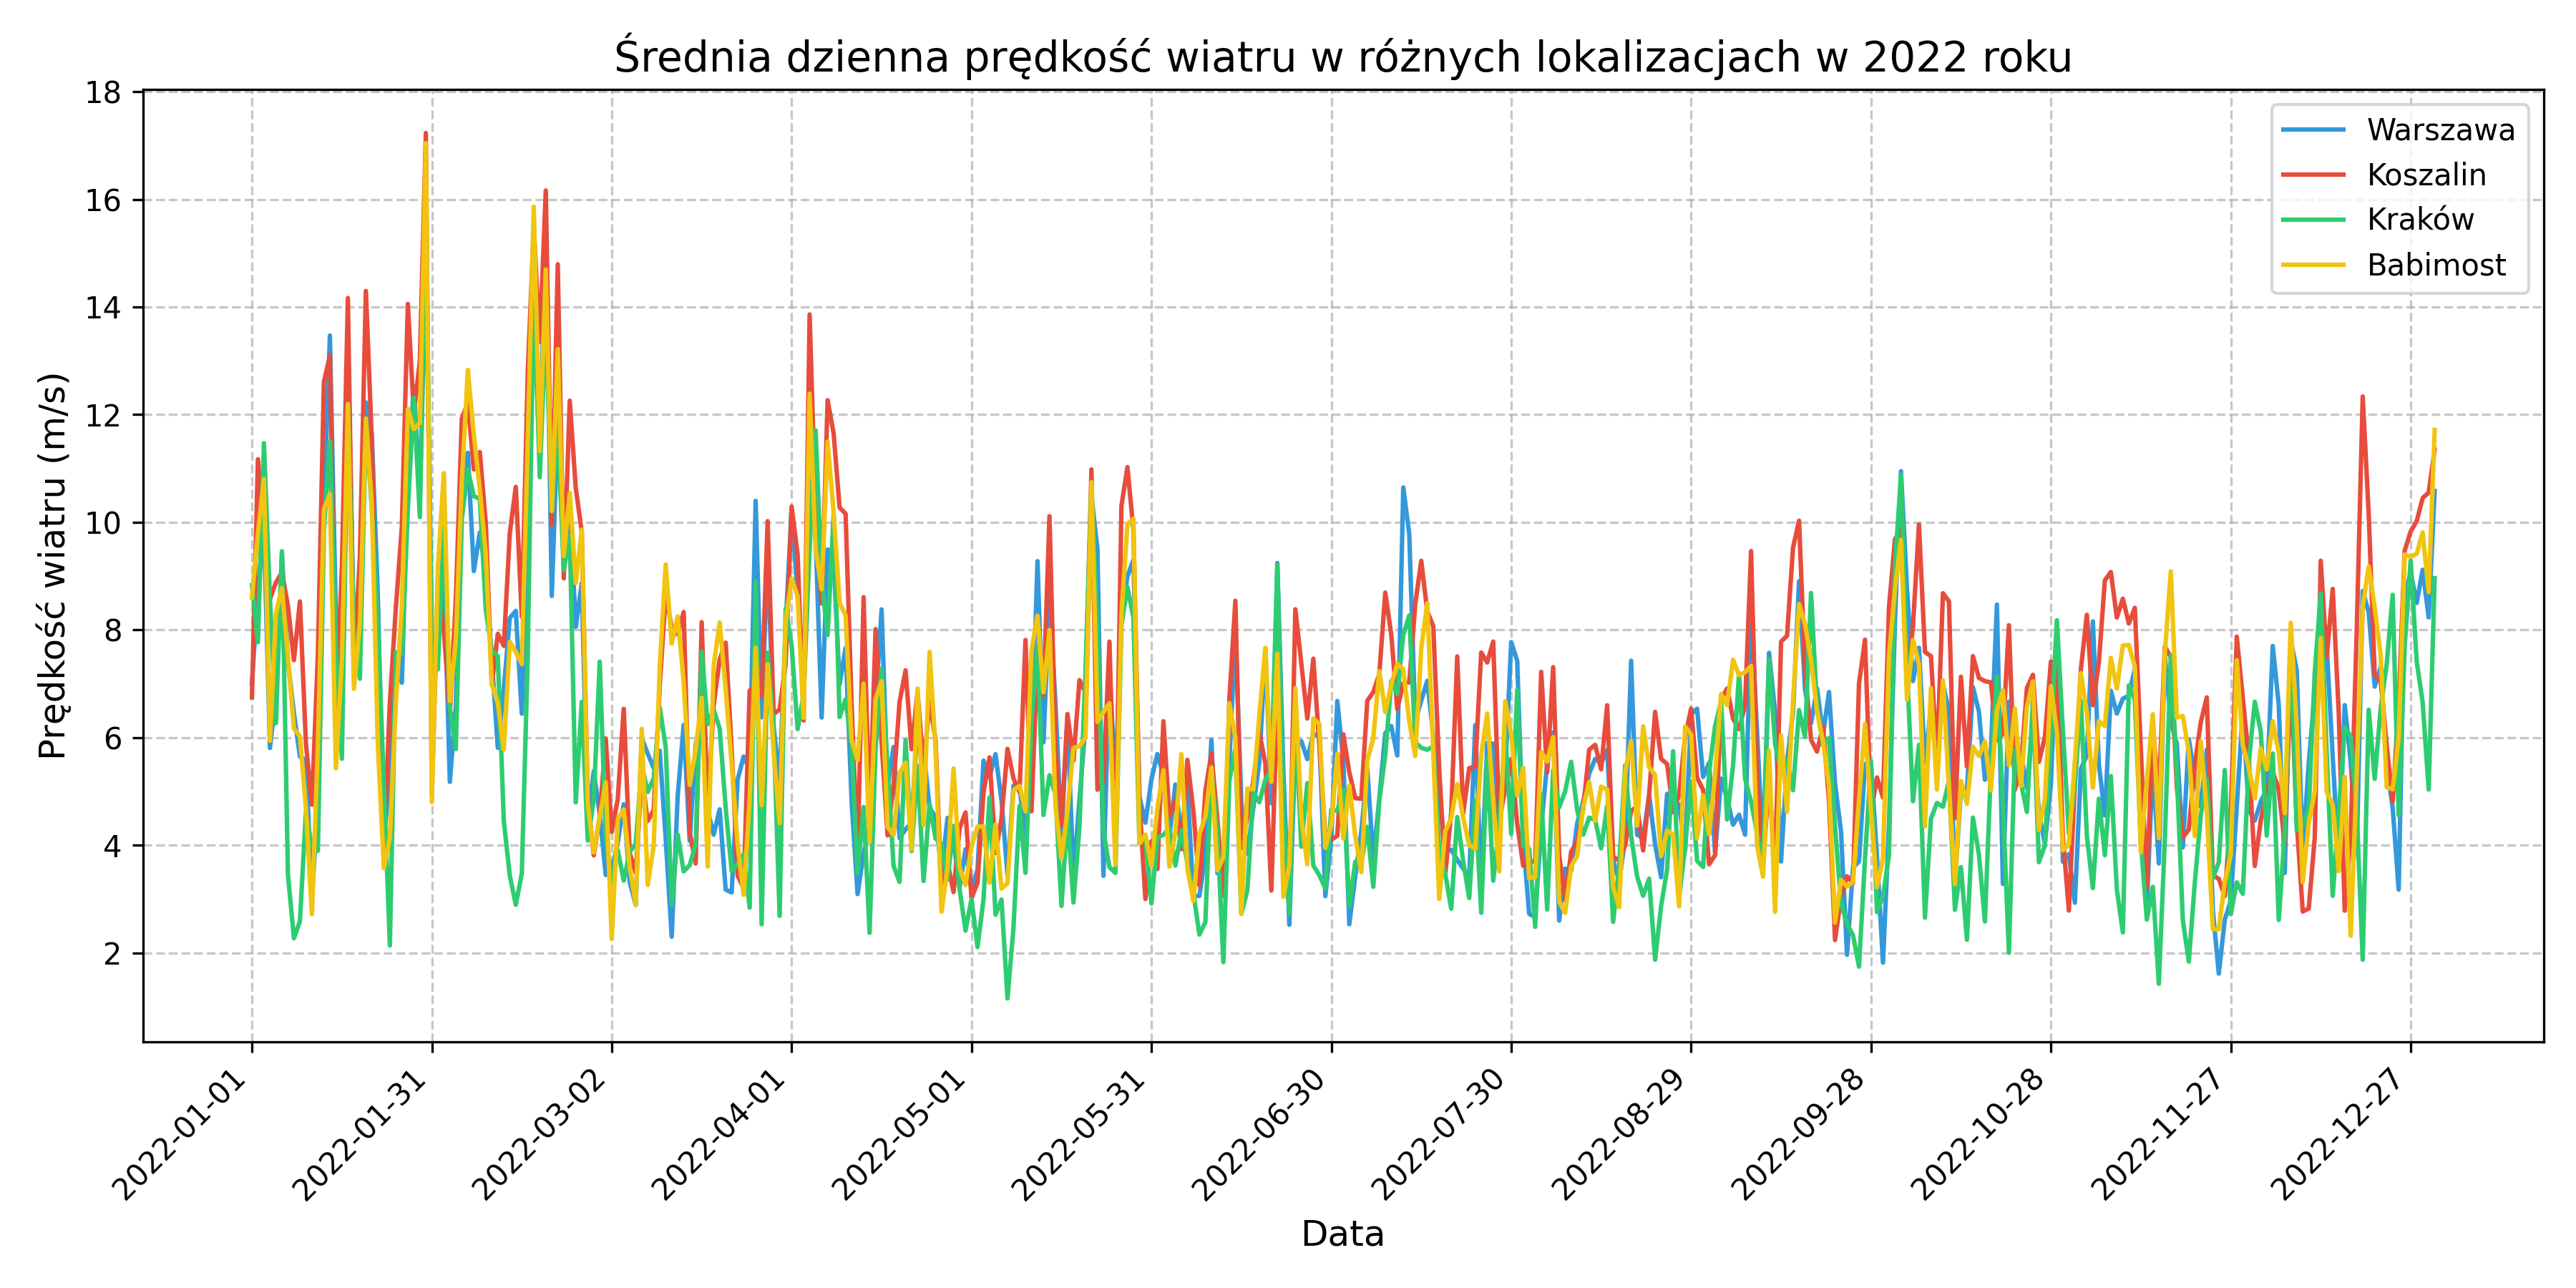
\includegraphics[width=\textwidth]{../plots/weather/wind_speed_time_series_2022.png}
    \caption{Zmienność prędkości wiatru w czasie (2022)}
    \label{fig:wind-speed-time-series-2022}
\end{figure}

\begin{figure}[H]
    \centering
    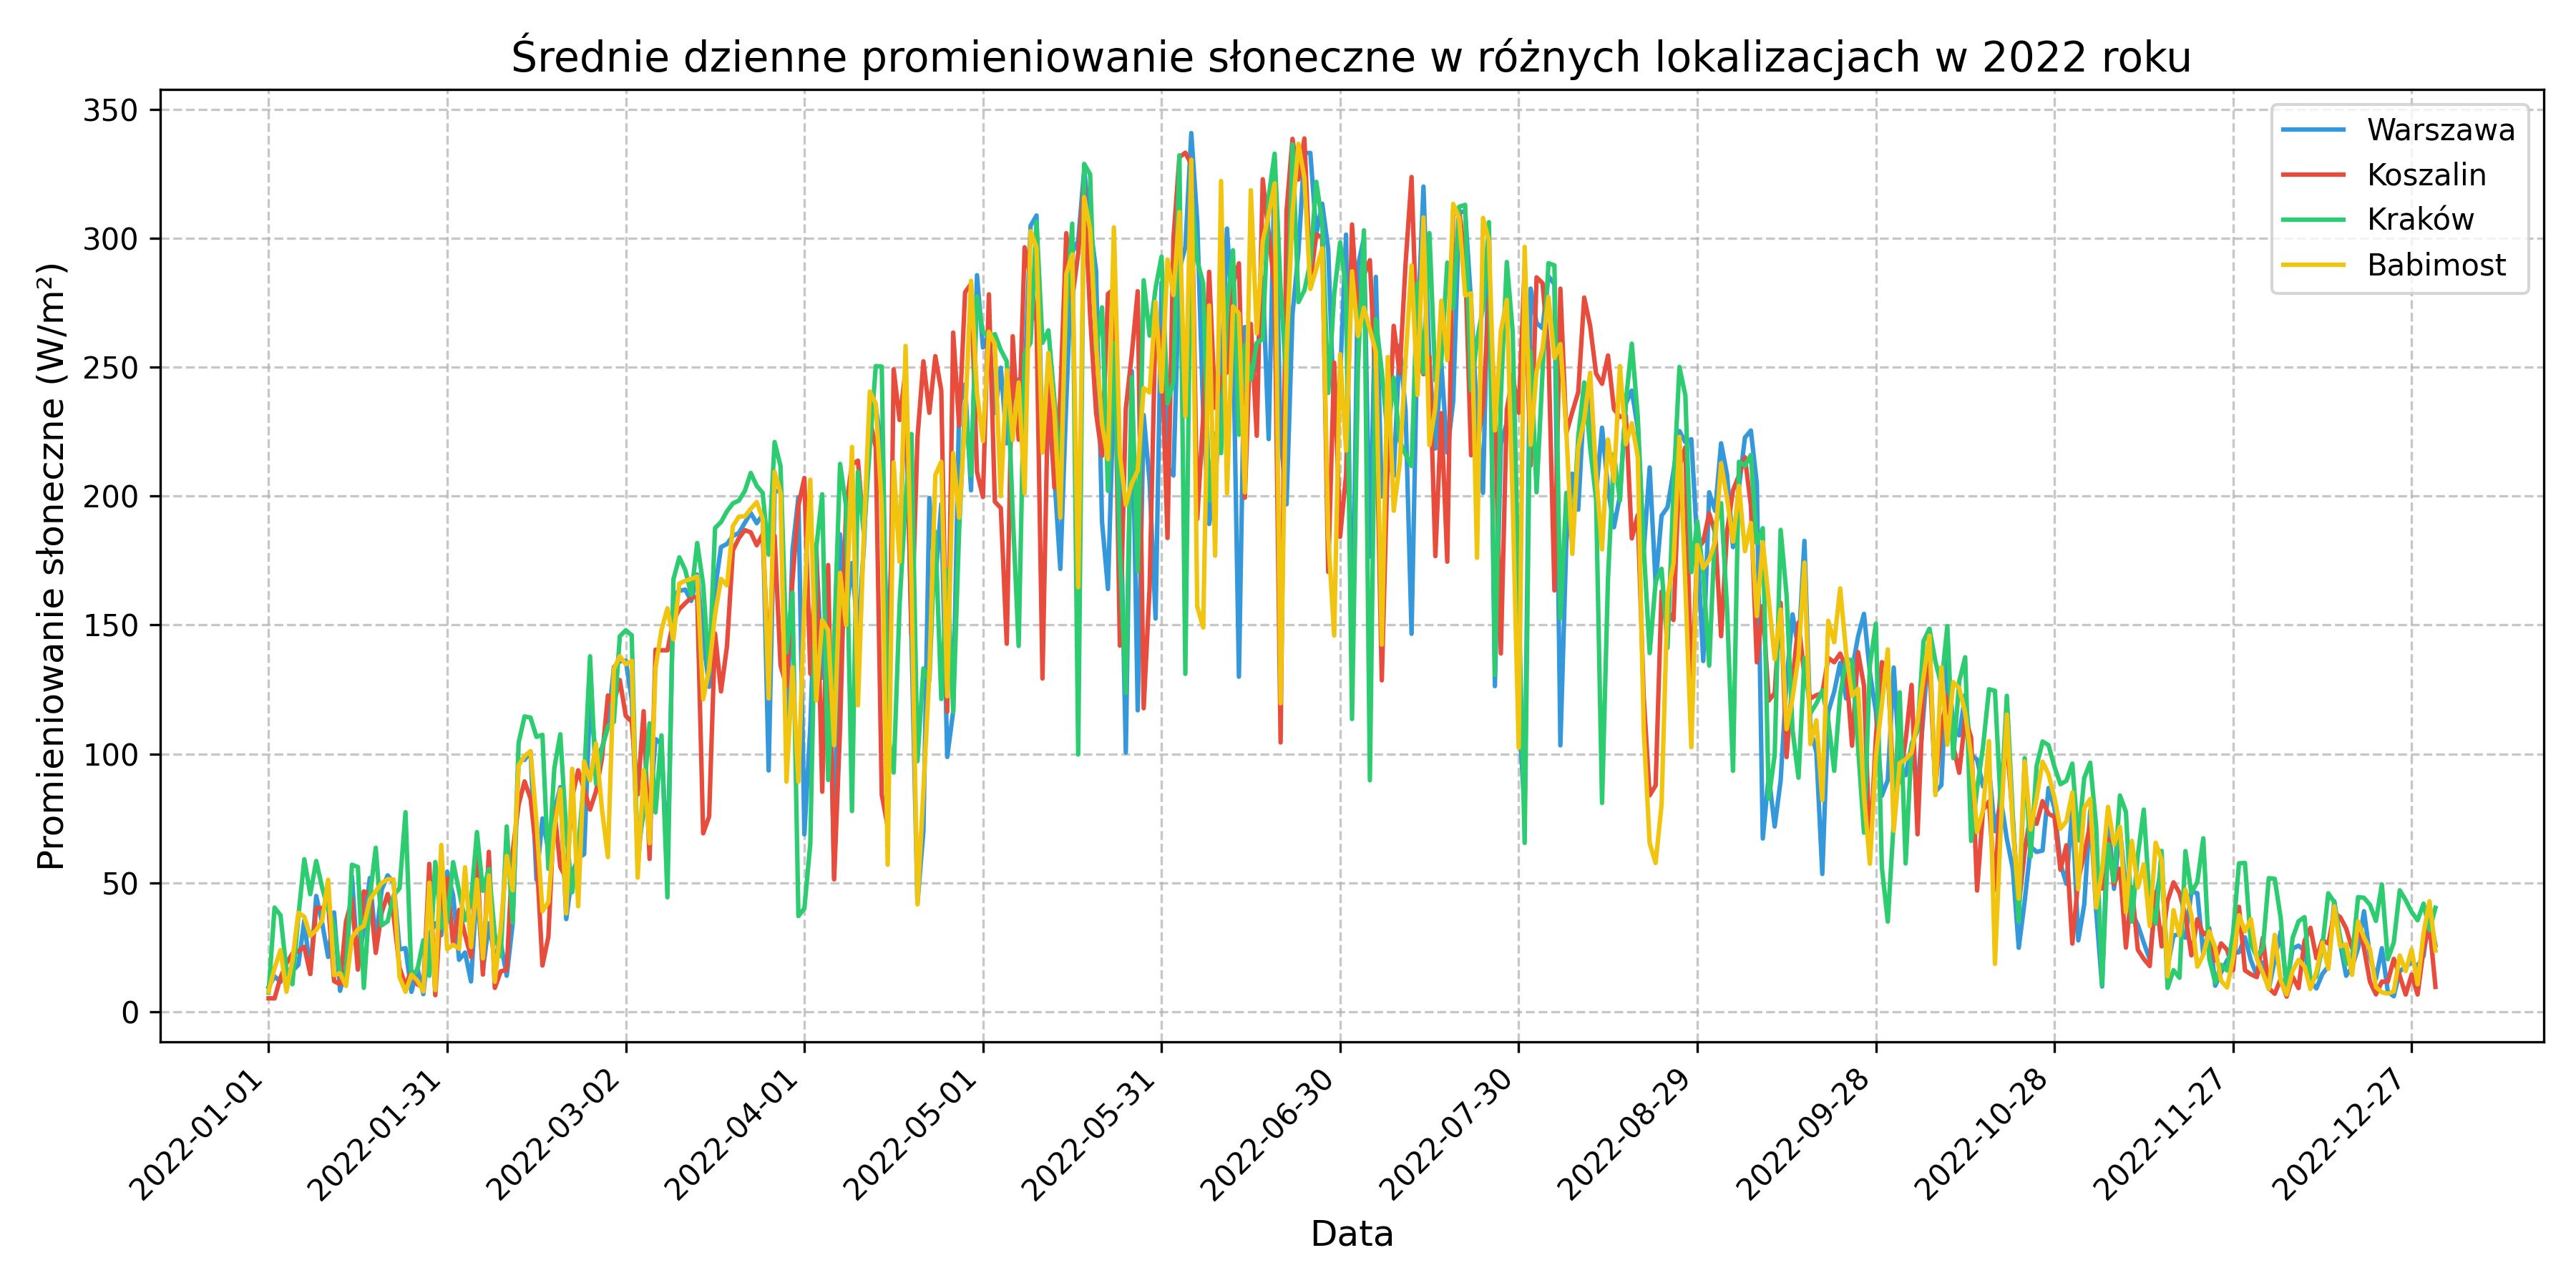
\includegraphics[width=\textwidth]{../plots/weather/solar_radiation_time_series_2022.png}
    \caption{Zmienność promieniowania słonecznego w czasie (2022)}
    \label{fig:solar-radiation-time-series-2022}
\end{figure}

\begin{figure}[H]
    \centering
    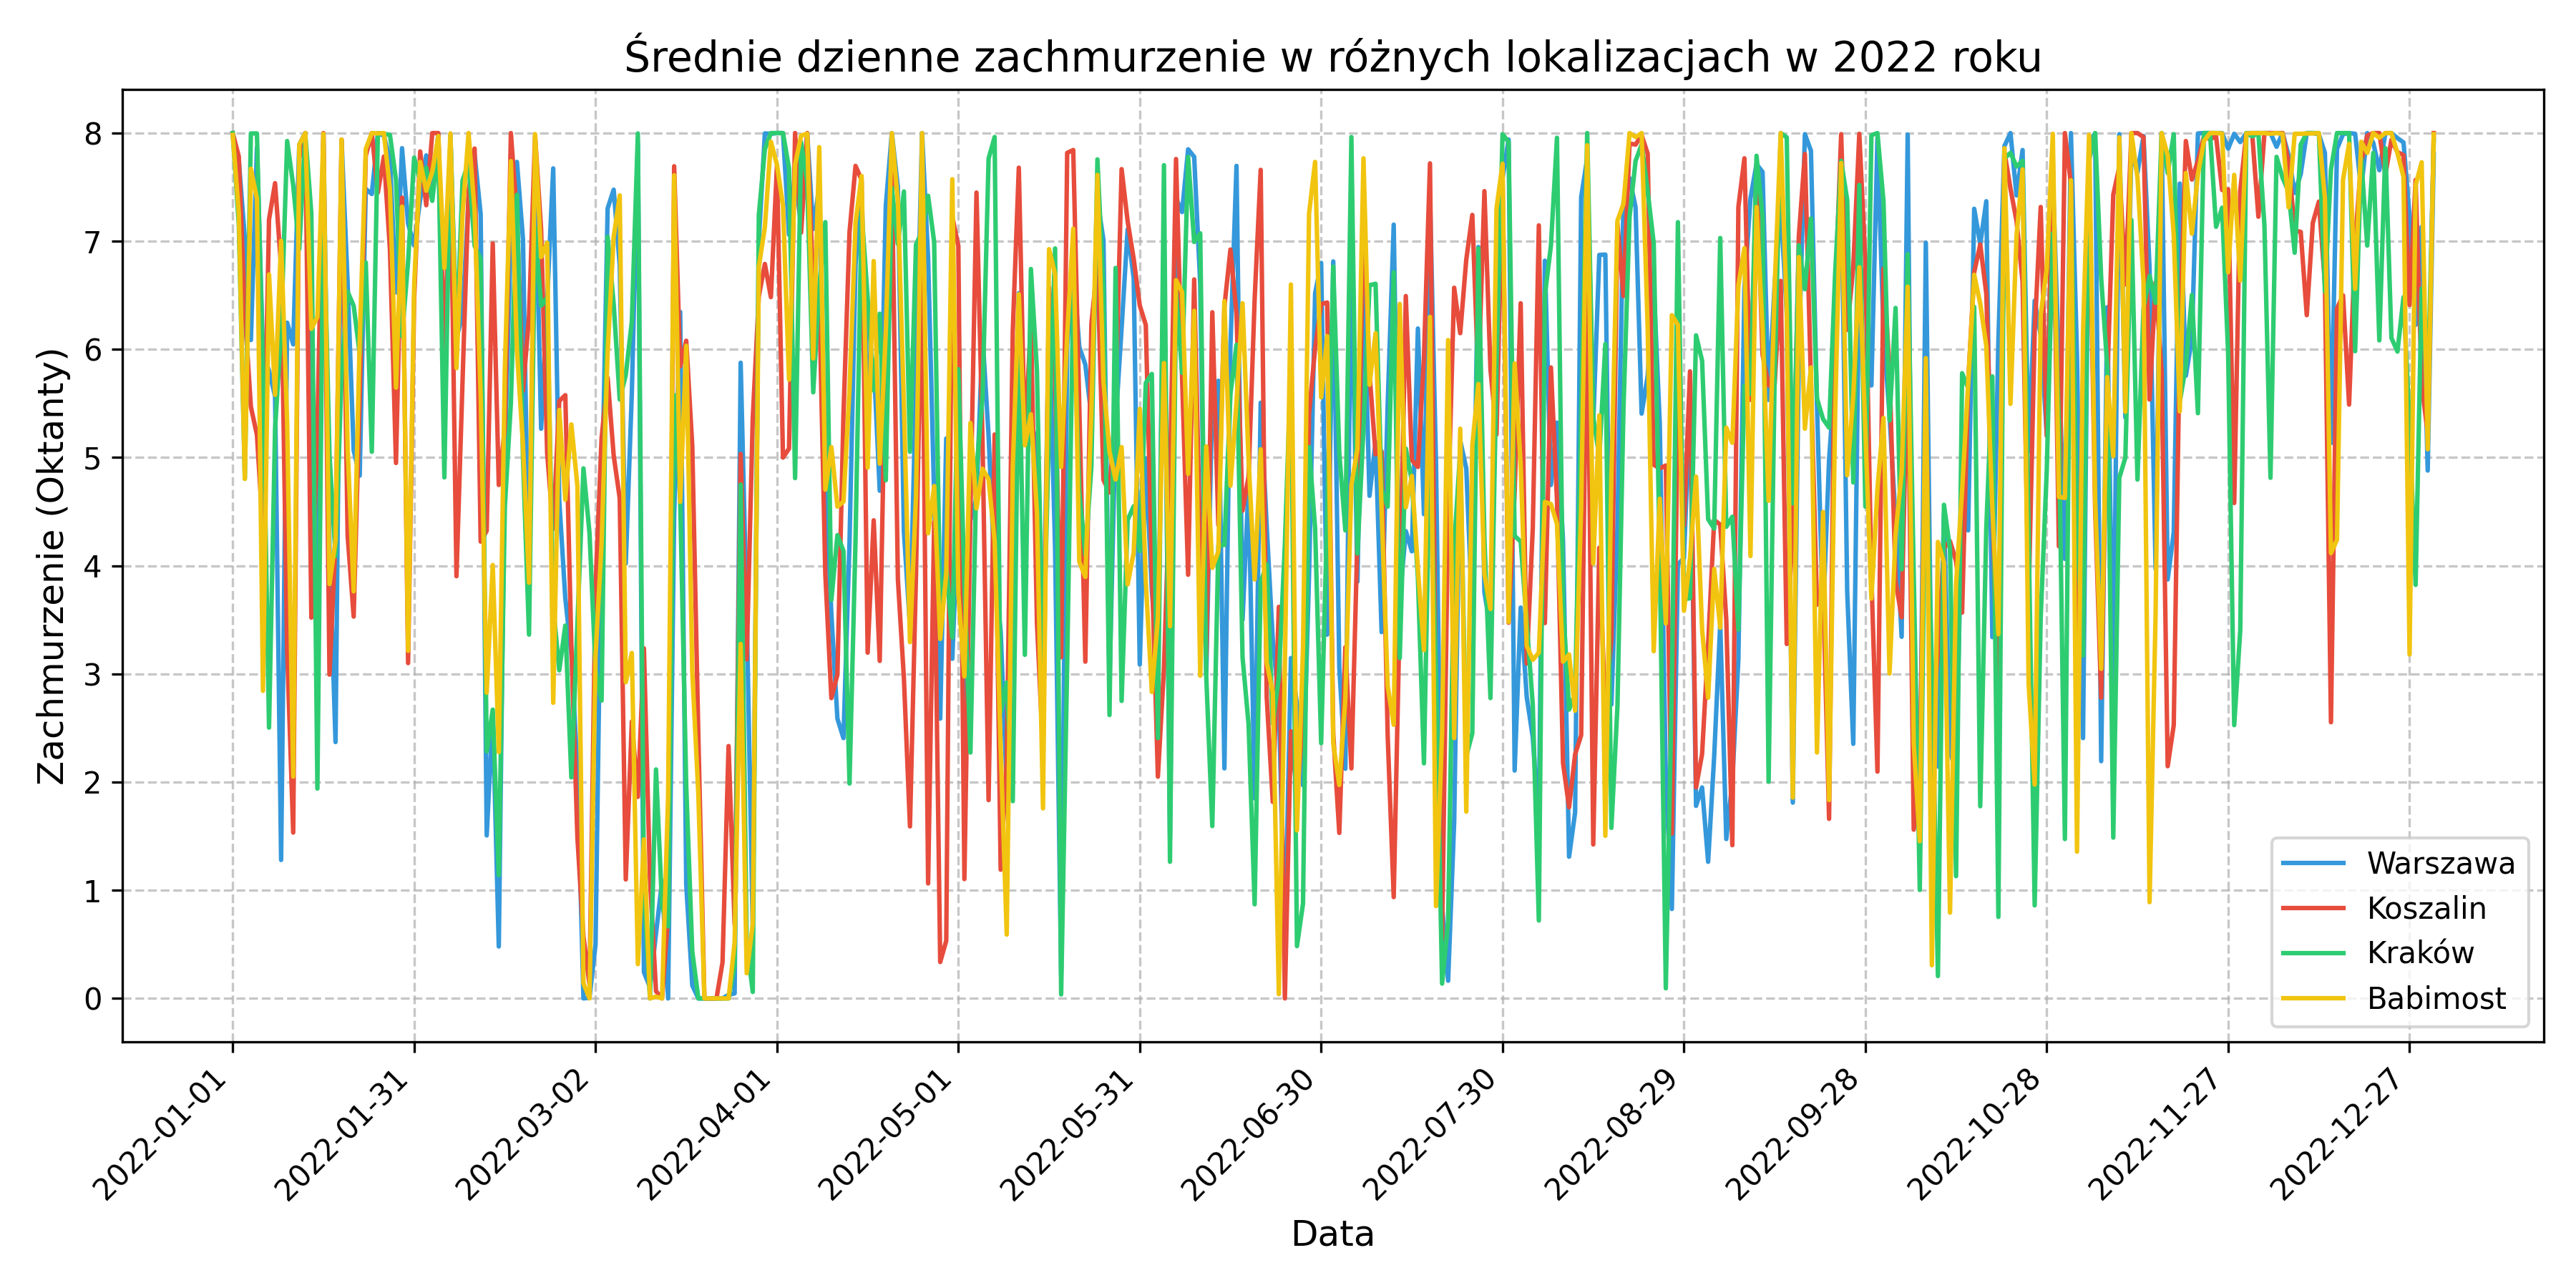
\includegraphics[width=\textwidth]{../plots/weather/cloud_cover_time_series_2022.png}
    \caption{Zmienność zachmurzenia w czasie (2022)}
    \label{fig:cloud-cover-time-series-2022}
\end{figure}

W ramach analizy w późniejszej części pracy spróbuję uprościć model i uśrednić wartości parametrów pogodowych dla całego kraju i sprawdzić czy wynik się poprawi. 

\subsection{Produkcja energii z wybranych źródeł}
Zmienne dotyczące produkcji energii z różnych źródeł odgrywają kluczową rolę w analizie cen energii na Rynku Dnia Następnego (RDN), ponieważ odzwierciedlają strukturę podaży energii w Polsce, która ma bezpośredni wpływ na dynamikę cen. W niniejszej pracy uwzględniono osiem zmiennych opisujących produkcję energii: 
\begin{itemize}
    \item \textbf{hard\_coal} - produkcja z węgla kamiennego (MW),
    \item \textbf{coal\_derived} - produkcja z paliw pochodnych węgla (MW),
    \item \textbf{lignite} - produkcja z węgla brunatnego (MW),
    \item \textbf{gas} - produkcja z gazu ziemnego (MW),
    \item \textbf{oil} - produkcja z ropy naftowej lub jej pochodnych (MW),
    \item \textbf{biomass} - produkcja z biomasy (MW),
    \item \textbf{wind} - produkcja z elektrowni wiatrowych lądowych (MW),
    \item \textbf{solar} - produkcja z paneli fotowoltaicznych (MW).
\end{itemize}

Dane te pochodzą z Polskich Sieci Elektroenergetycznych (PSE) i zostały dopasowane do godzinowego formatu danych RDN, co pozwoliło na ich integrację z pozostałymi zmiennymi. 
\begin{figure}[H]
    \centering
    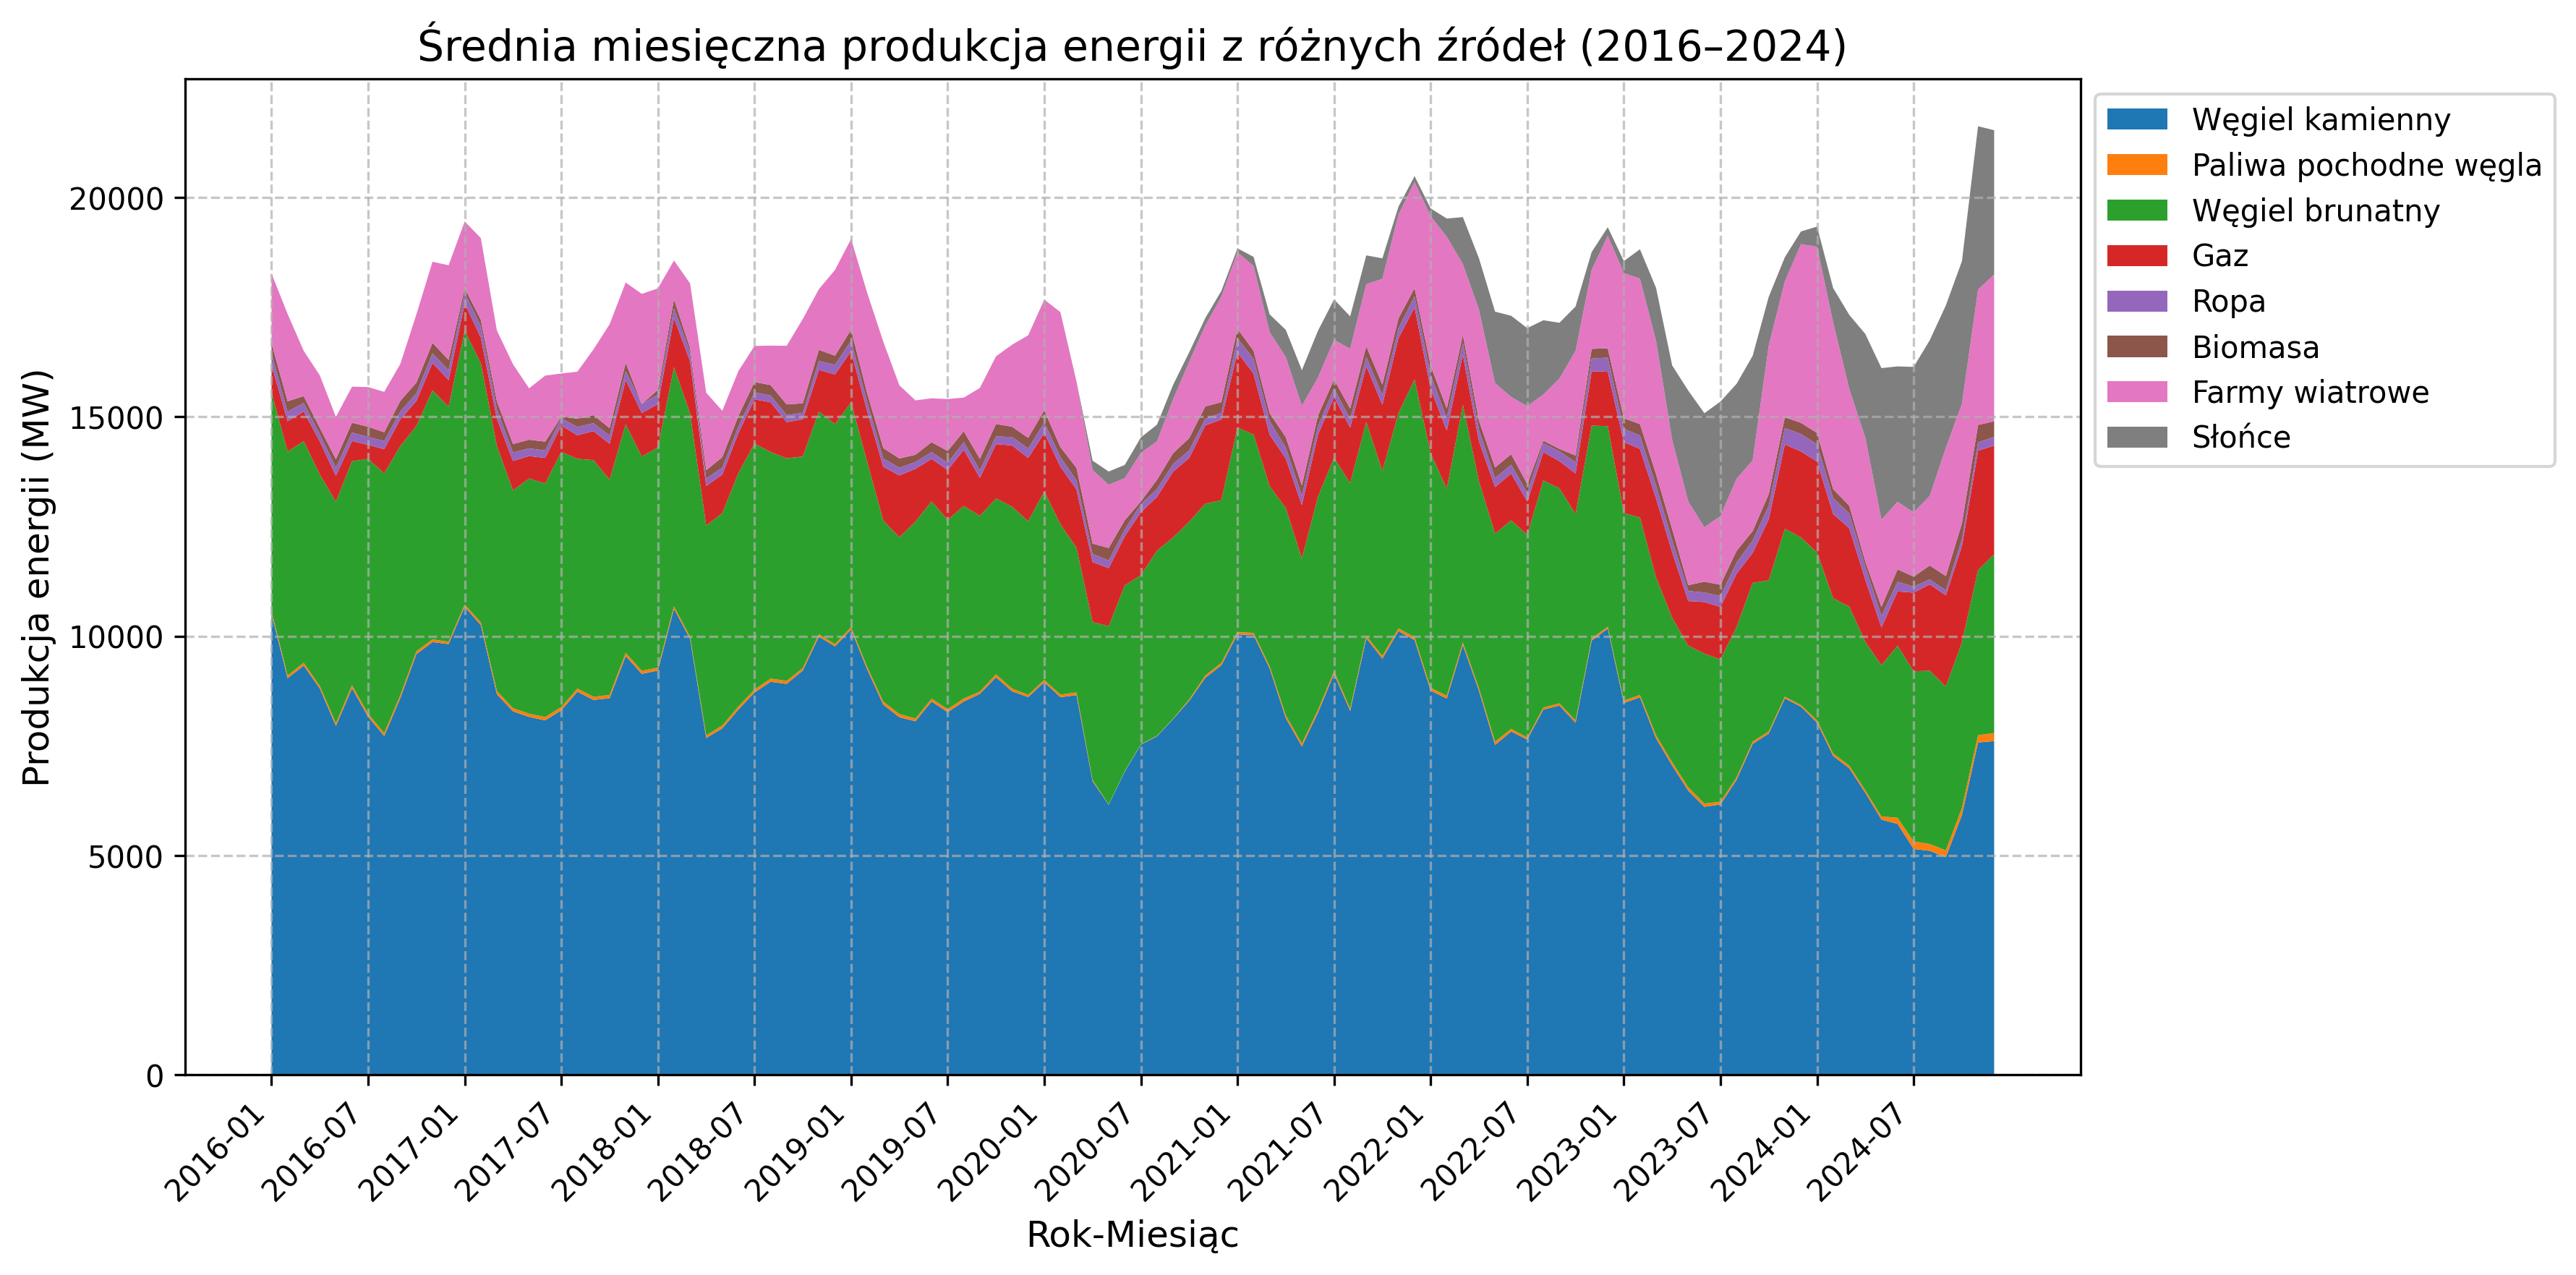
\includegraphics[width=1.05\textwidth]{../plots/energy/energy_production_time_series_full.png}
    \caption{Zmienność produkcji energii z różnych źródeł w czasie (2016–2024)}
    \label{fig:energy-production-time-series-full}
\end{figure}

Wykres powyżej przedstawia średnią miesięczną produkcję energii z różnych źródeł w Polsce w latach 2016–2024, co jest istotne w kontekście prognozowania cen energii (EPF) na Rynku Dnia Następnego (RDN). Wykres obszarowy ukazuje dominację węgla kamiennego i brunatnego, której do tej pory odpowiadają za większość produkcji energii elektrycznej. Biomasa oraz paliwa pochodne węgla stanowią znikomą część podaży i mogą być pominięte dla redukcji ilości zmiennych. Produkcja za pomocą gazu i ropy stale posiada niewielką, ale istotną część produkcji energii. Warto zauważyć, że produkcja z OZE, szczególnie ze słońca znacząco rośnie w ostatnich latach, co może mieć istotny wpływ na ceny energii i umiejętność jej prognozowania. 
\begin{figure}[H]
    \centering
    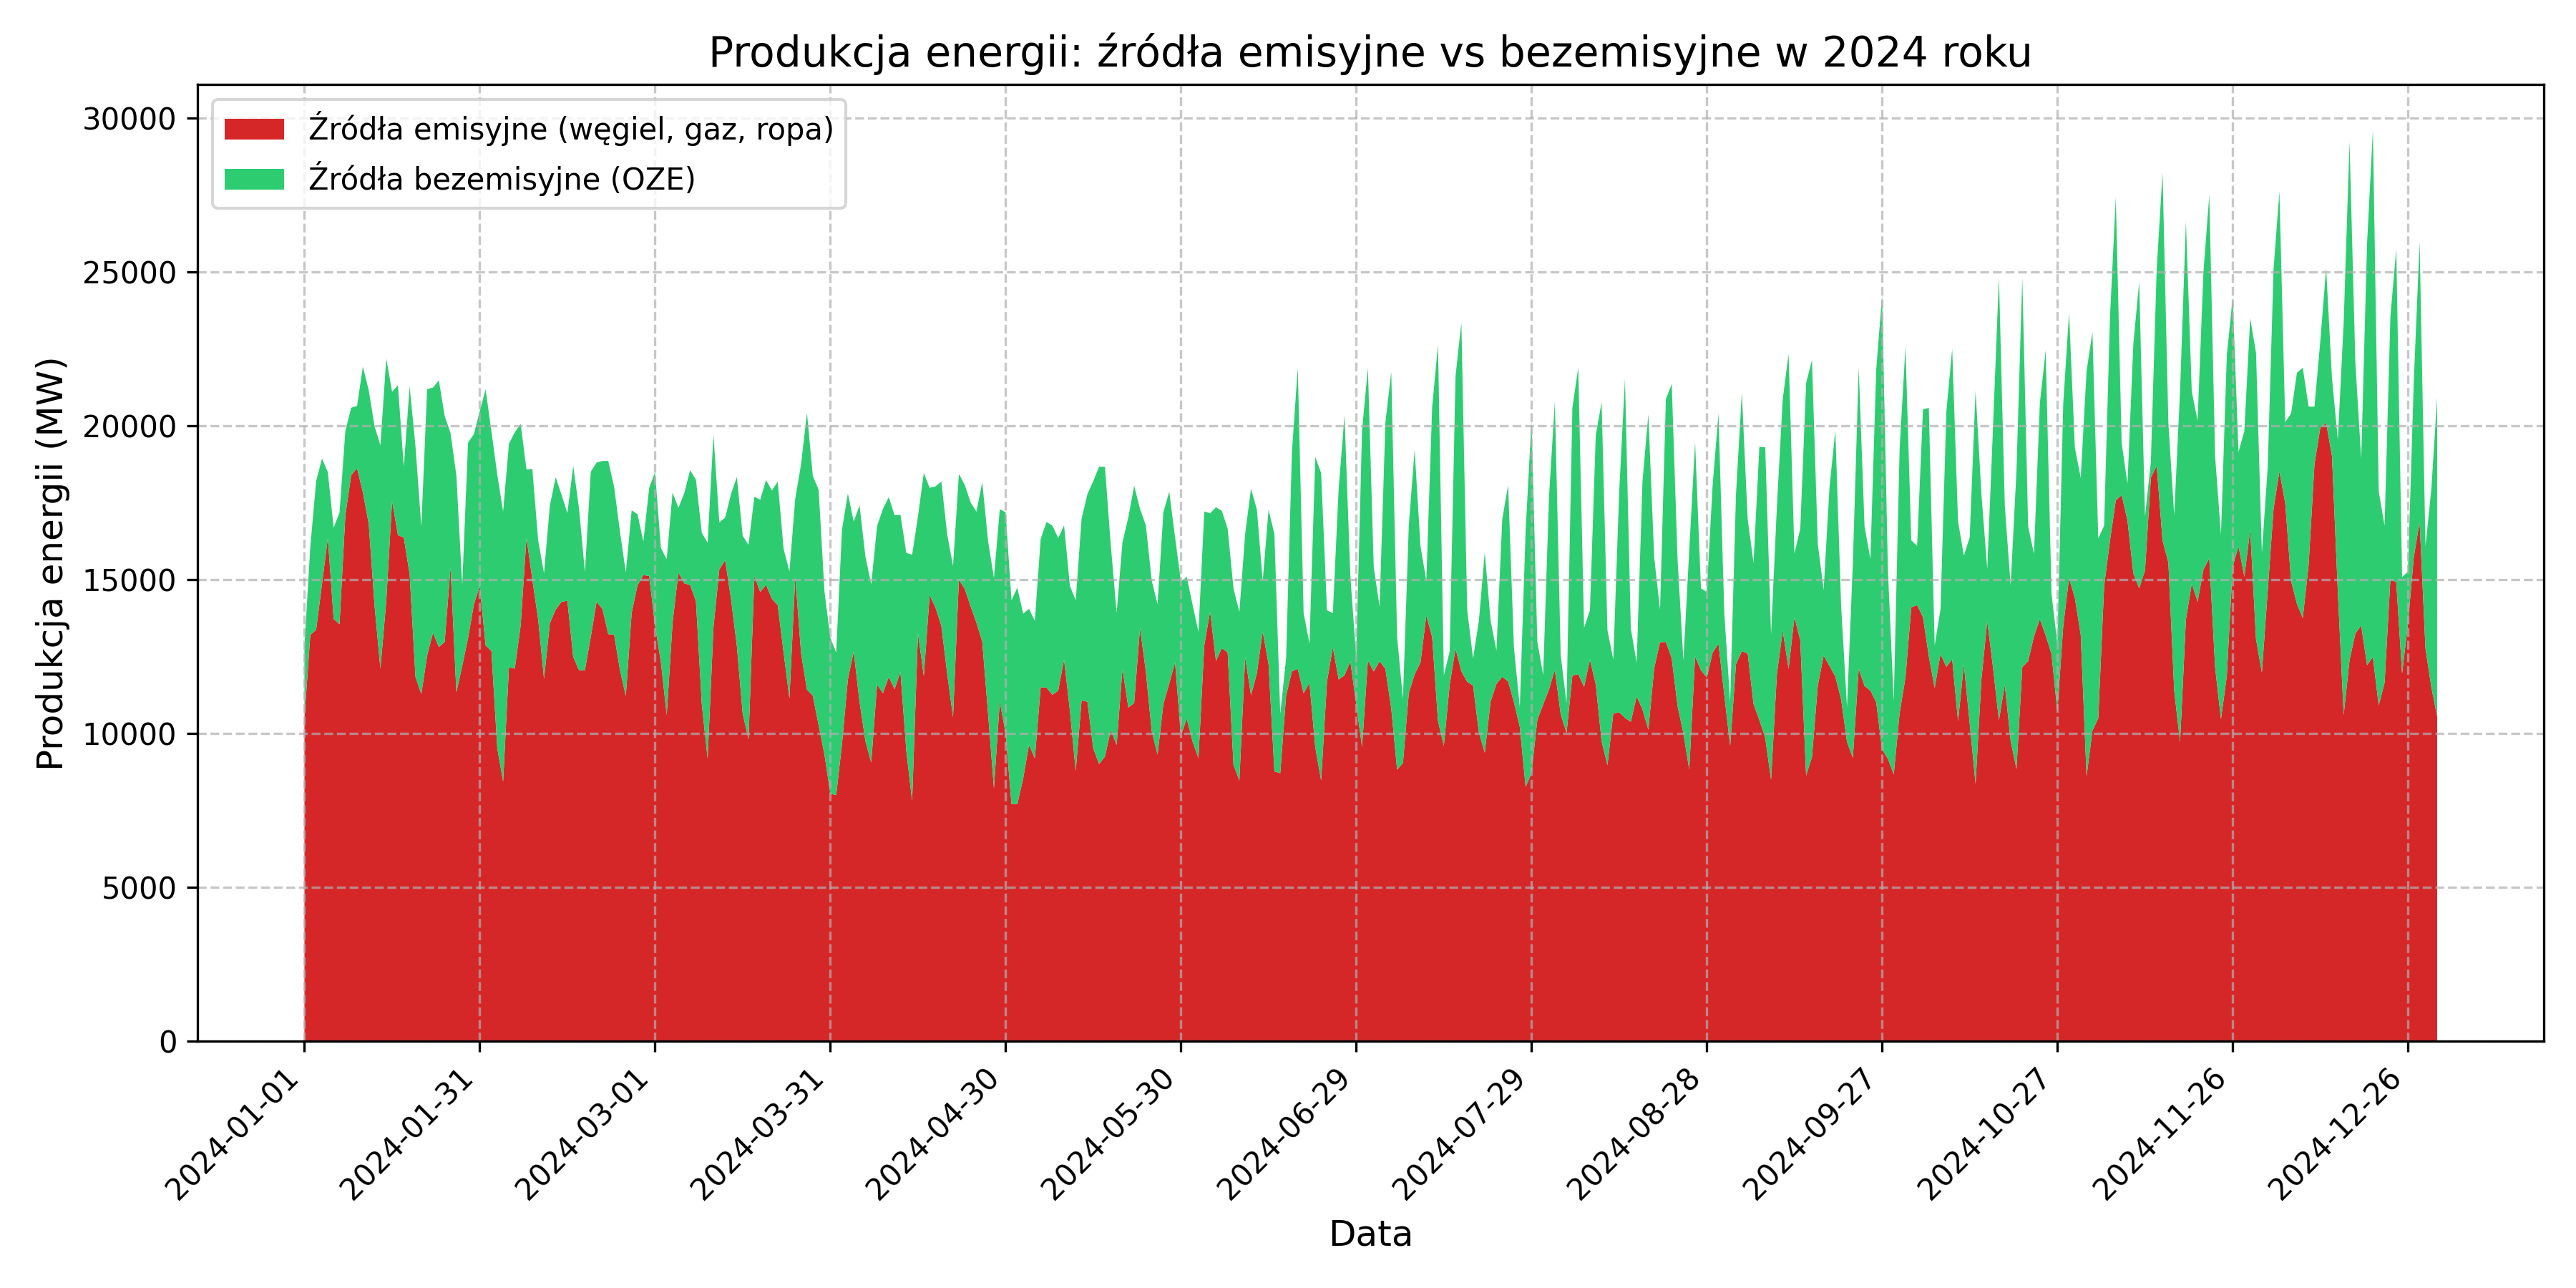
\includegraphics[width=\textwidth]{../plots/energy/emission_vs_non_emission_2024.png}
    \caption{Porównanie produkcji energii z emisyjnych i bezemisyjnych źródeł w 2024 roku}
    \label{fig:emission-vs-non-emission-2024}
\end{figure}
W najbardziej korzystne dla gospodatki momenty część produkcji z OZE może przekraczać zapewnienie energii z węgla, co może prowadzić do spadku cen energii. Warto również zauważyć, że produkcja z węgla kamiennego i brunatnego jest bardziej stabilna i przewidywalna niż produkcja z OZE, co może wpływać na dokładność prognoz. W związku z tym, zmienne dotyczące produkcji energii z różnych źródeł są istotnym elementem analizy i modelowania cen energii na RDN.

\subsection{Handel energią z państwami sąsiednimi}
\label{subsec:trade}
Zmienne dotyczące wymiany energii z innymi krajami są istotnym elementem analizy cen energii na Rynku Dnia Następnego (RDN), ponieważ pozwalają na uwzględnienie wpływu handlu międzynarodowego na ceny energii w Polsce. W niniejszej pracy uwzględnione zostały bilanse handlu energią z Państwami sąsiednimi, z którymi Polska ma połączenia transgraniczne. Są to Państwa takie jak:
\begin{itemize}
    \item Niemcy (DE),
    \item Czechy (CZ),
    \item Słowacja (SK),
    \item Litwa (LT),
    \item Szwecja (SE),
    \item Ukraina (UA).
\end{itemize}

Dane dotyczące wymiany energii z tymi krajami pochodzą z Polskich Sieci Elektroenergetycznych (PSE) i są dostępne w granulacji godzinowej. Warto zauważyć, że Polska jest jednym z kluczowych graczy na rynku energii w Europie Środkowo-Wschodniej, a wymiana energii z innymi krajami może mieć istotny wpływ na ceny energii w Polsce. W szczególności, w okresach wysokiego zapotrzebowania na energię lub w sytuacjach poważnych awarii, Polska może importować energię z innych krajów, co prowadzi do wzrostu cen. Z drugiej strony, w okresach niskiego zapotrzebowania, Polska może eksportować, czyli sprzedawać nadwyżki energii, co może prowadzić do spadku cen. Poniżej przedstawiam wykresy dotyczące wymiany energii z sąsiadami w latach 2016-2024.

\begin{table}[H]
    \centering
    \resizebox{\textwidth}{!}{%
    \begin{tabular}{|c|r|r|r|r|r|r|}
    \hline
    \textbf{Rok} & \textbf{Niemcy (MW)} & \textbf{Czechy (MW)} & \textbf{Litwa (MW)} & \textbf{Słowacja (MW)} & \textbf{Szwecja (MW)} & \textbf{Ukraina (MW)} \\ \hline
    2016 & 994.26  & -761.81 & 68.21   & -475.47 & 294.36  & 108.99  \\ \hline
    2017 & 836.24  & -612.73 & 119.92  & -499.21 & 340.96  & 102.45  \\ \hline
    2018 & 803.00  & -373.78 & 102.53  & -366.14 & 310.83  & 160.96  \\ \hline
    2019 & 1149.22 & -312.31 & 216.38  & -367.32 & 329.80  & 157.17  \\ \hline
    2020 & 1275.75 & -264.90 & 201.93  & -348.95 & 428.81  & 167.98  \\ \hline
    2021 & 957.79  & -901.92 & 110.04  & -519.59 & 364.69  & 93.55   \\ \hline
    2022 & 918.62  & -1000.89 & 86.53  & -684.25 & 429.17  & 126.95  \\ \hline
    2023 & 851.27  & -526.46 & 58.40   & -382.18 & 431.60  & 5.76    \\ \hline
    2024 & 1005.26 & -544.15 & -112.90 & -389.65 & 296.29  & -68.03  \\ \hline
    \end{tabular}%
    }
    \caption{Średni bilans wymiany energii z sąsiadami w latach 2016–2024}
    \label{tab:energy-trade-balance}
\end{table}

Wartości te są średniogodzinowymi bilansami wymiany energii z sąsiadami w latach 2016-2024. Wartości dodatnie oznaczają eksport energii, a wartości ujemne import energii. Polska ma dodatni bilans wymiany energii z Niemcami, co oznacza, że Polska regularnie eksportuje energię do Niemiec. Największe ujemne bilanse Polska posiada z Czechami, prawdopodobnie spowodowane jest to funkcjonującymi w Czechami elektrowniami atomowymi. Te przepływy wpływają na ceny na RDN: eksport do Niemiec i Szwecji może podnosić ceny w Polsce, a import z Czech i Słowacji stabilizuje system, ale zwiększa zależność od zewnętrznych dostawców.

\subsection{Ceny paliw kopalnych i emisji CO2}
\label{subsec:prices}

Zmienne dotyczące cen paliw kopalnych oraz emisji CO$_2$ odgrywają kluczową rolę w analizie cen energii na Rynku Dnia Następnego (RDN), ponieważ koszty paliw i emisji mają bezpośredni wpływ na ceny energii elektrycznej w Polsce, gdzie dominującym źródłem energii jest węgiel. W niniejszej pracy uwzględniono cztery zmienne, które zostały opisane w Tabeli~\ref{tab:fuel_variables}.

\begin{table}[H]
    \centering
    \begin{tabular}{|l|l|l|l|}
    \hline
    \textbf{Nazwa zmiennej} & \textbf{Opis} & \textbf{Źródło danych} & \textbf{Granulacja} \\ \hline
    \texttt{gas\_price}     & Cena gazu ziemnego (PLN/MWh) & energy.instrat.pl & Dzienna \\ \hline
    \texttt{coal\_price}    & Cena węgla kamiennego (PLN/GJ) & energy.instrat.pl & Dzienna \\ \hline
    \texttt{co2\_price}     & Cena uprawnień do emisji CO$_2$ (PLN/tCO$_2$) & energy.instrat.pl & Dzienna \\ \hline
    \texttt{brent\_price}   & Cena ropy Brent Europe (PLN/bar) & www.eia.gov & Dzienna \\ \hline
    \end{tabular}
    \caption{Opis zmiennych dotyczących cen paliw kopalnych i emisji CO$_2$.}
    \label{tab:fuel_variables}
\end{table}

Dane te zostały dopasowane do godzinowego formatu danych RDN, w taki sposób, że w dniach pracy giełdy i znanych cen paliw, cena stale jest przypisana do godzin, a w dniach wolnych od pracy lub bez znanych cen, wartości są interpolowane. 

Ceny paliw kopalnych i emisji CO$_2$ są istotne w kontekście prognozowania cen energii, ponieważ wpływają na koszty produkcji energii w elektrowniach konwencjonalnych, które dominują w polskim miksie energetycznym. Na przykład, wzrost ceny węgla (\texttt{coal\_price}) lub uprawnień do emisji CO$_2$ (\texttt{co2\_price}) zwiększa koszty produkcji energii w elektrowniach węglowych. Cena gazu (\texttt{gas\_price}) jest kluczowa dla elektrowni gazowych, które pełnią rolę bilansującą w systemie. Cena ropy Brent (\texttt{brent\_price}) ma mniejszy bezpośredni wpływ na produkcję energii w Polsce, ale jest istotna w kontekście globalnych trendów cen paliw, które mogą wpływać na inne zmienne, takie jak cena gazu.

Aby zilustrować dynamikę tych zmiennych, na rysunku poniżej przedstawiono zmiany cen paliw kopalnych i emisji CO$_2$ w latach 2016--2024 w ujęciu miesięcznym. Dla lepszego przedstawienia danych użyłem skali logarytmicznej.

\begin{figure}[h]
    \centering
    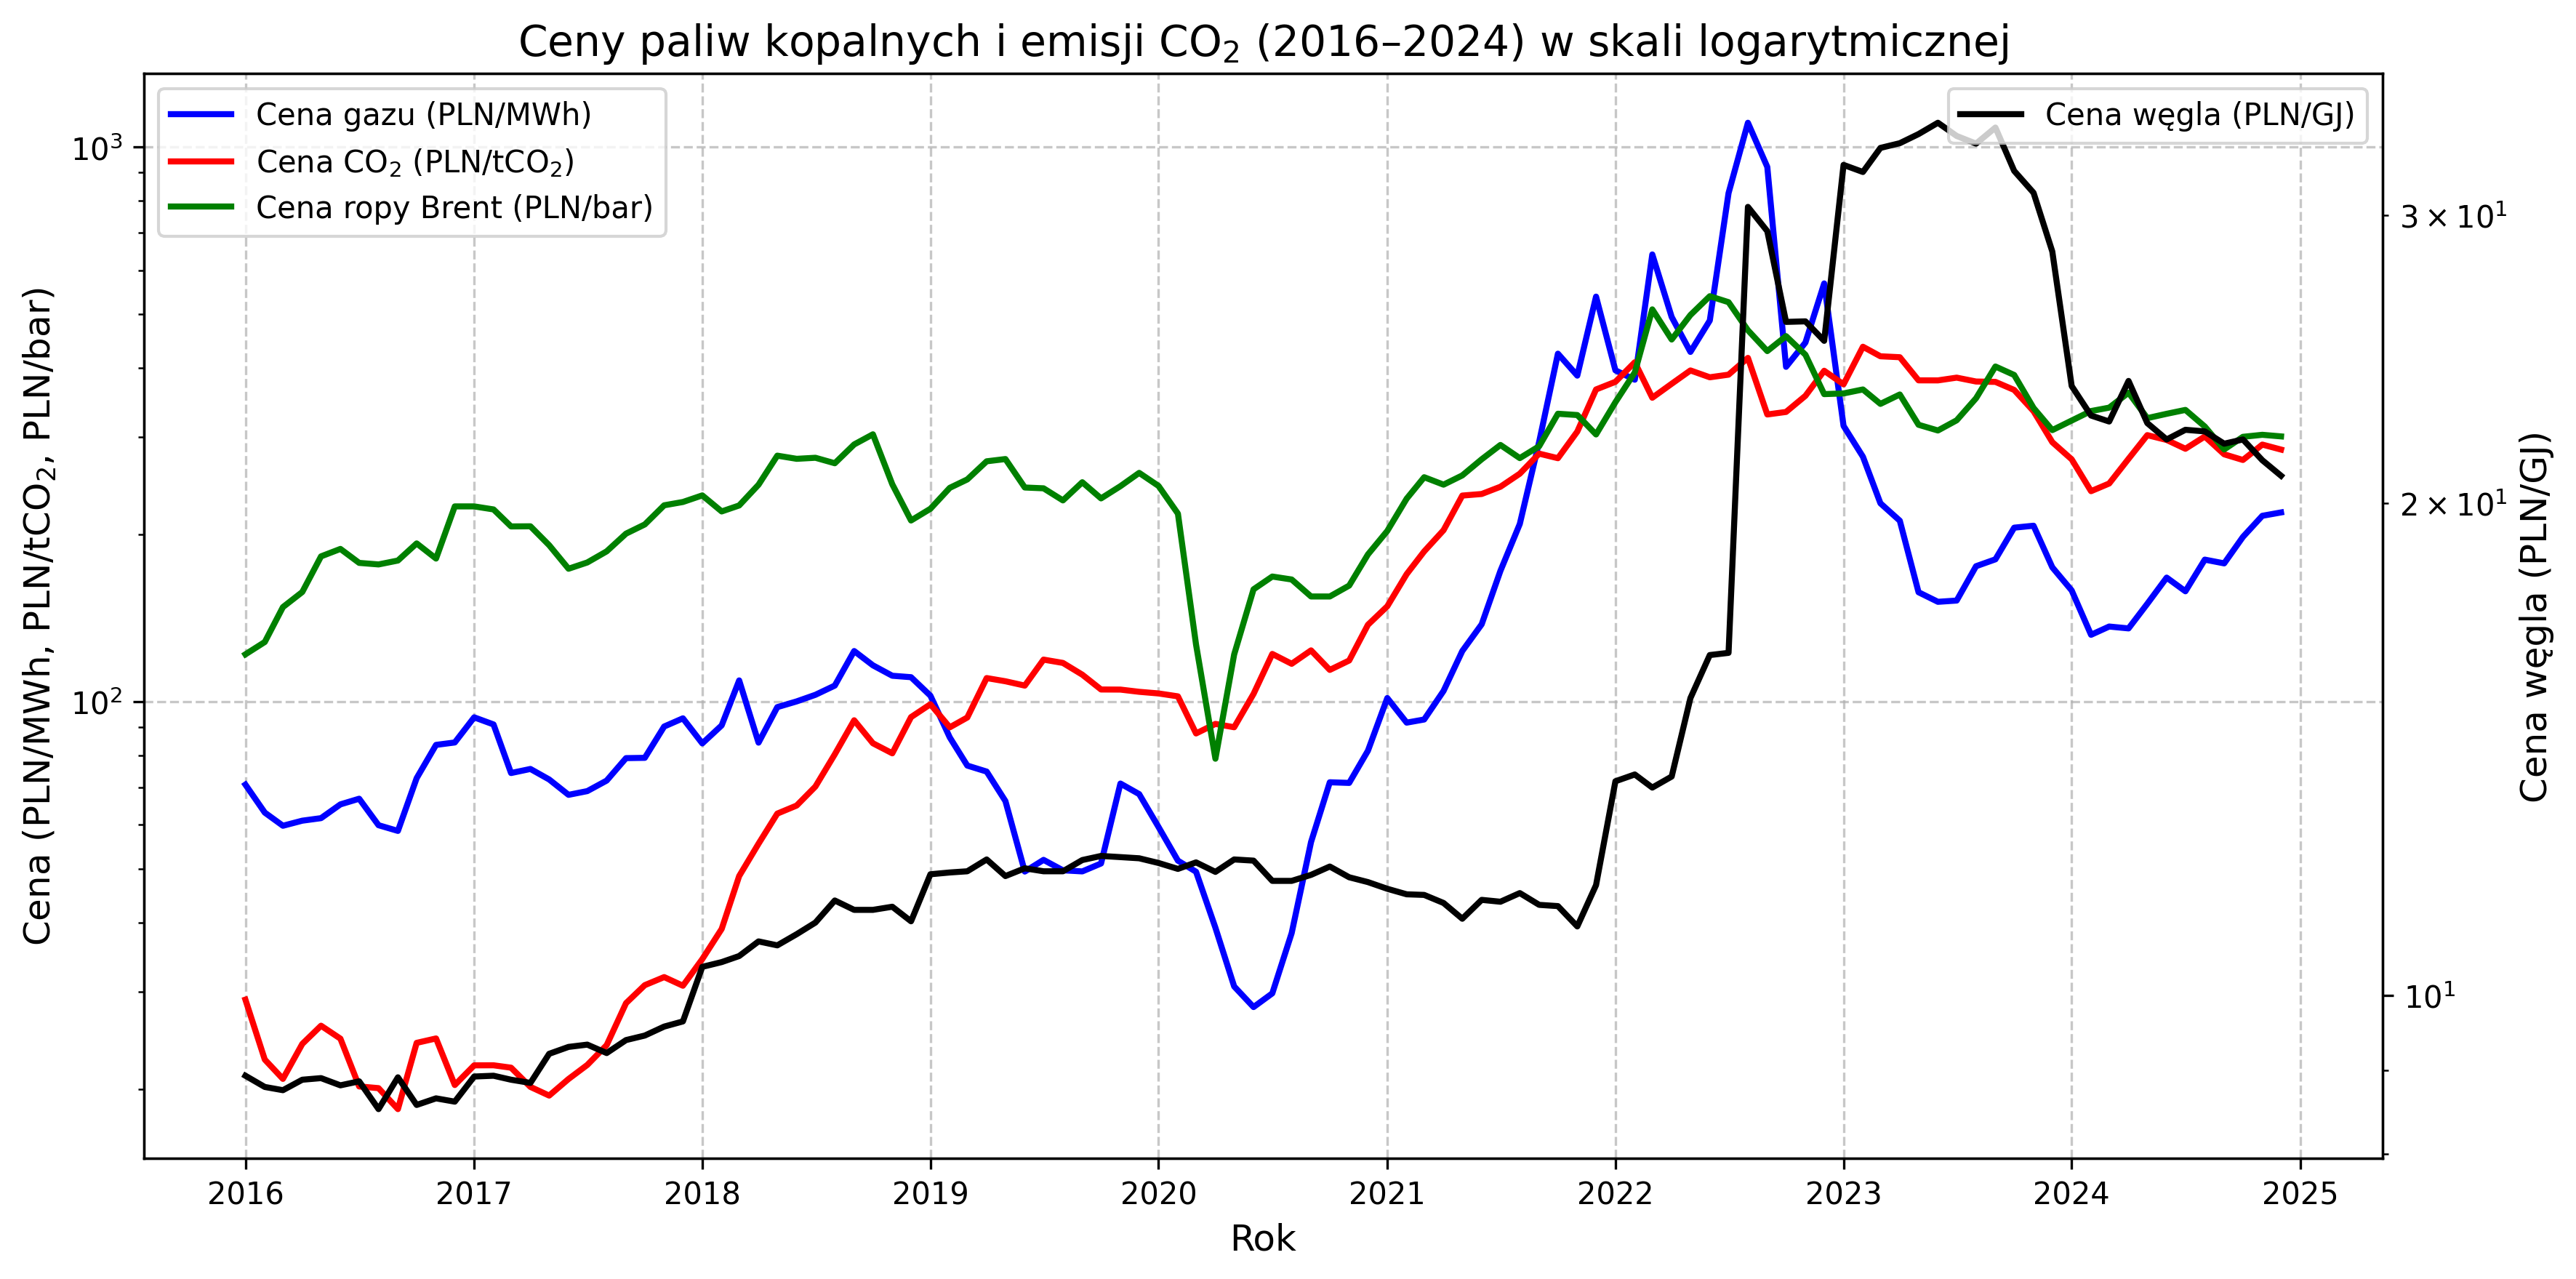
\includegraphics[width=0.9\textwidth]{../plots/fuels/fuel_prices_2016_2024.png}
    \caption{Ceny paliw kopalnych i emisji CO$_2$ w latach 2016--2024 (w ujęciu miesięcznym). Źródło: Opracowanie własne na podstawie danych rynkowych.}
    \label{fig:fuel_prices}
\end{figure}

Ceny paliw kopalnych w okresie wysokiej zmienności szybko rosną, co prawdopodobnie jest przyczyną rosnących cen energii. Największy wzrost ma cena gazu, która od rozpoczęcia konfliktu zbrojnego wzrosła ponad 10-krotnie w ciągu roku. 

\subsection{Straty mocy w systemie elektroenergetycznym}
\label{subsec:losses}

Zmienne dotyczące strat mocy w systemie elektroenergetycznym odgrywają istotną rolę w analizie cen energii na Rynku Dnia Następnego (RDN), ponieważ wpływają na dostępność energii w systemie oraz koszty jej przesyłu i dystrybucji. W niniejszej pracy uwzględniono następujące dane zbierane przez systemy PSE: \texttt{power\_loss} (utrata mocy w wyniku awarii w MW) oraz \texttt{network\_loss} (utrata mocy w sieci w MW). Udostępnione dane mają granulację godzinową. 

Straty mocy w systemie elektroenergetycznym są kluczowe w kontekście prognozowania cen energii, ponieważ zmniejszają ilość energii dostępnej dla odbiorców, co może prowadzić do wzrostu cen na RDN oraz \gls{rb}. Utrata mocy w wyniku awarii

Aby zilustrować dynamikę tych zmiennych, na rysunku~\ref{fig:power_losses} przedstawiono zmiany strat mocy w wyniku awarii (\texttt{power\_loss}) oraz strat mocy w sieci (\texttt{network\_loss}) w latach 2016--2024 w ujęciu miesięcznym.

\begin{figure}[h]
    \centering
    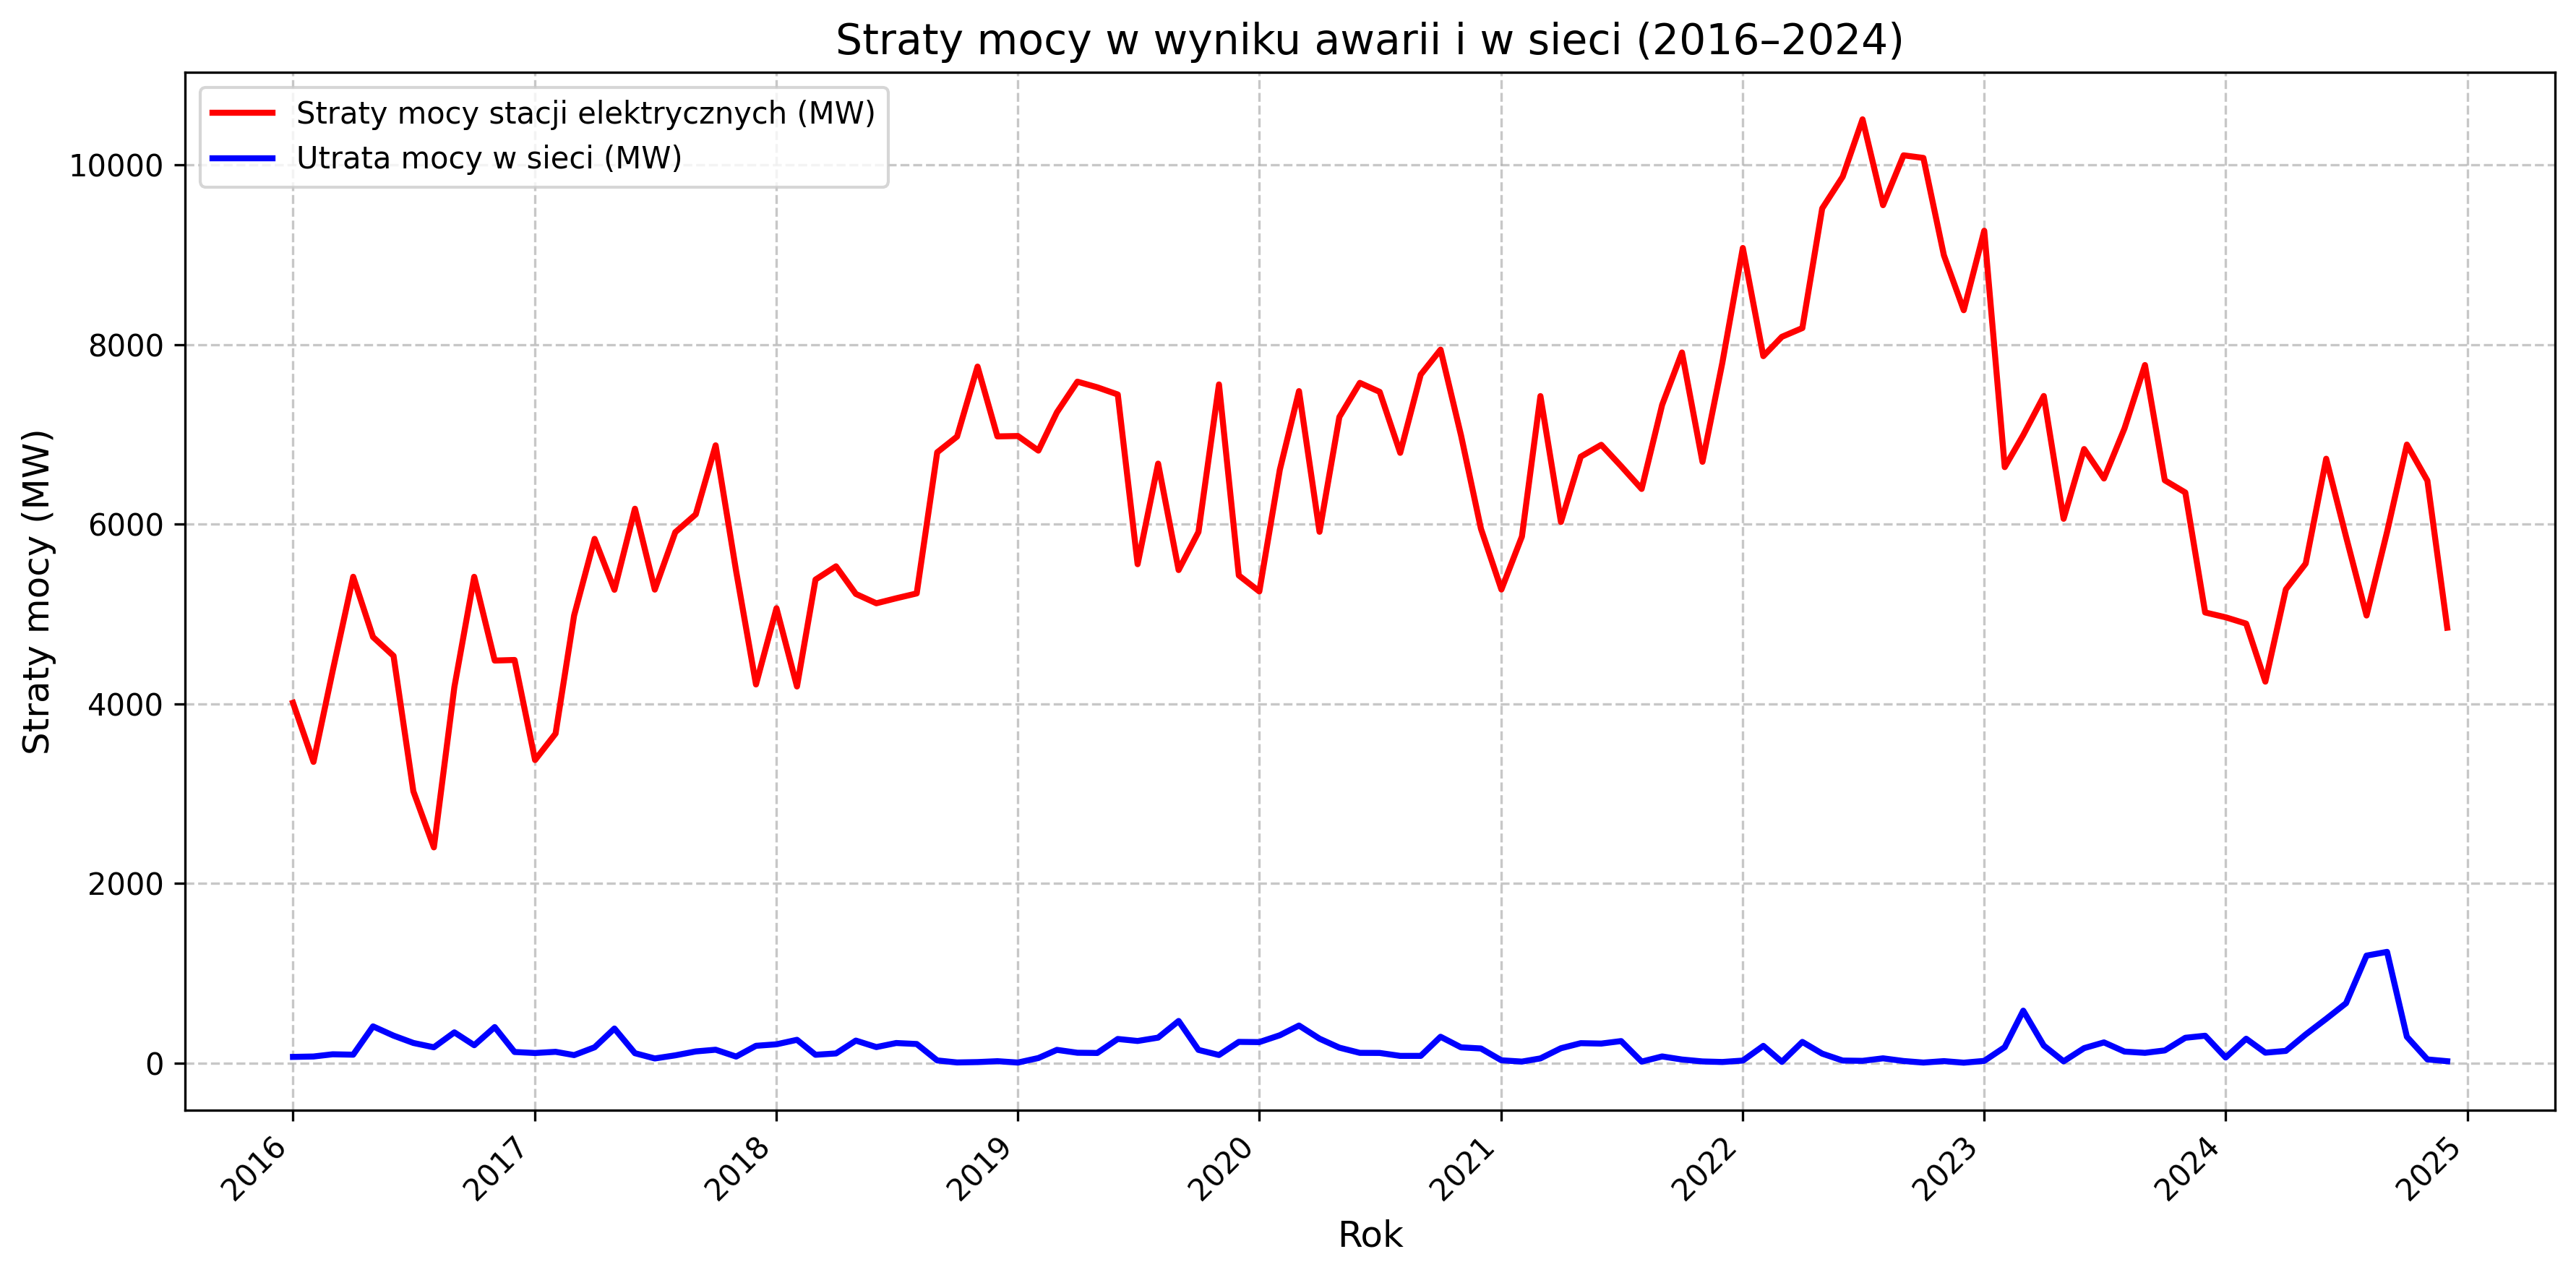
\includegraphics[width=0.9\textwidth]{../plots/losses/power_losses_2016_2024.png}
    \caption{Straty mocy w wyniku awarii i w sieci w latach 2016--2024 (w ujęciu miesięcznym). Źródło: Opracowanie własne na podstawie danych z PSE.}
    \label{fig:power_losses}
\end{figure}

Straty sieciowe na wykresie po 06.2024 są większe od poprzednich. Wynika to ze zmiany metodyki obliczania strat sieciowych przez PSE. Niemniej jednak straty mocy są znaczące, ale wynikają prawdopodbnie z tego, że nie wszystkie jednostki wytworcze pracują w danym momencie lub z ograniczonej ich eksploatacji. 

\subsection{Zapotrzebowanie na energię i wolumen handlu}
\label{subsec:demand}

Zmienne dotyczące zapotrzebowania na energię i wolumenu handlu są kluczowe w analizie cen energii na Rynku Dnia Następnego (RDN), ponieważ mają bezpośredni wpływ na równowagę między podażą a popytem, co jest podstawowym czynnikiem kształtującym ceny energii. W niniejszej pracy uwzględniono następujące zmienne: \texttt{load} (zapotrzebowanie na energię w MWh) oraz \texttt{trade\_volume} (wolumen handlu w MWh). Obie zmienne pochodzą z Polskich Sieci Elektroenergetycznych (PSE) i są dostępne w granulacji godzinowej.

Poniżej na wspólnym wykresie przedstawię różnice pomiędzy zapotrzebowaniem a wolumenem handlu.

\begin{figure}[H]
    \centering
    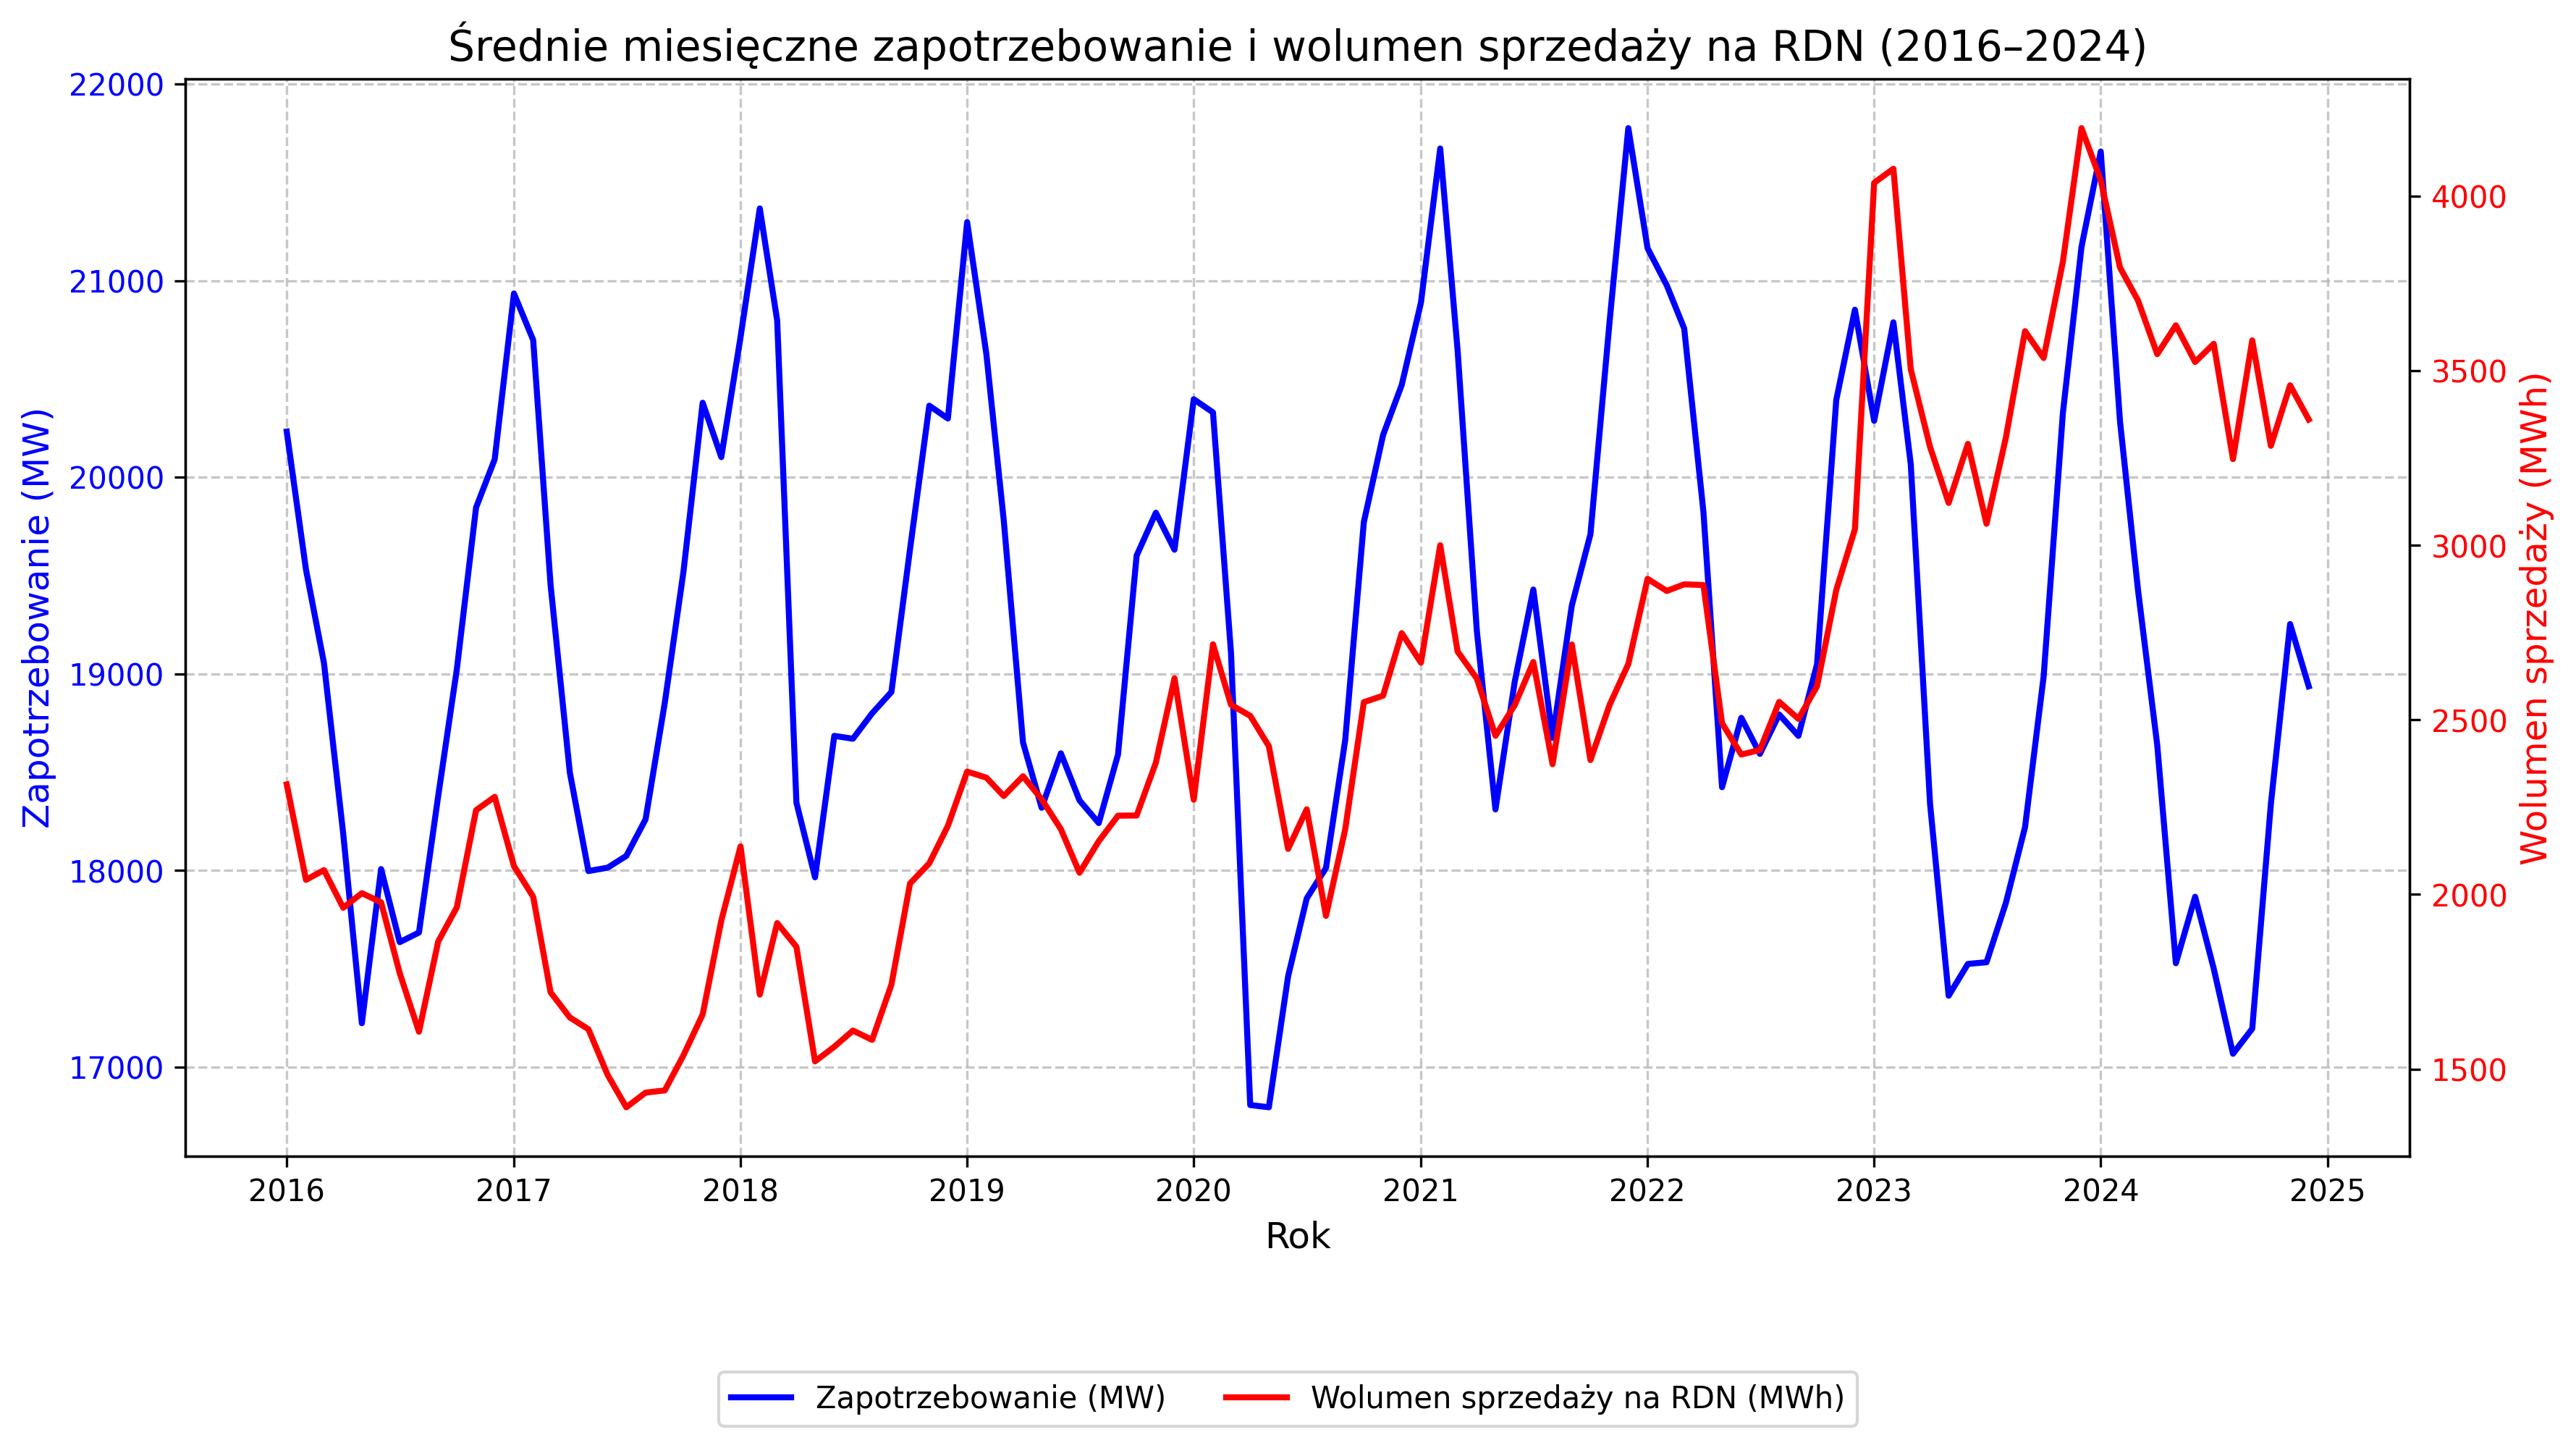
\includegraphics[width=0.9\textwidth]{../plots/market/load_vs_volume_2016_2024.png}
    \caption{Zapotrzebowanie na energię i wolumen handlu w latach 2016--2024 (w ujęciu miesięcznym). Źródło: Opracowanie własne na podstawie danych z PSE.}
    \label{fig:load_vs_trade_volume}
\end{figure}

Rozbieżność między zapotrzebowaniem a wolumenem sprzedaży na RDN ma swój powód. Wolumen sprzedaży na RDN zwykle nie przekracza 5000 MWh w porównaniu do zapotrzebowania na poziomie ponad 15 000  MWh wskazuje, że RDN pokrywa jedynie część \% całkowitego zapotrzebowania. Pozostała część jest zaspokajana przez: (1) kontrakty bilateralne (OTC), (2) rynek bilansujący, na którym PSE kupuje energię w czasie rzeczywistym, (3) import energii z sąsiednich krajów, jak pokazano w podrozdziale~\ref{subsec:trade} oraz innego rodzaju transakcje. 

Wyraźnie widoczne są duże szczyty zapotrzebowania zapotrzebowania w okresie zimowym. Wynika to z zwiększonego zapotrzebowania na energię elektryczną w okresie grzewczym, co jest typowe dla klimatu Polski.

\subsection{Inne zmienne}
\label{subsec:seasonal}

W swoim zbiorze danych uwzględnione zostały inne zmienne, które mogą mieć wpływ na ceny energii na RDN.

\subsubsection{Zmienne sezonowe}
\label{subsubsec:seasonal_variables}
Zmienne sezonowe, takie jak \texttt{day\_of\_week}, \texttt{month} i \texttt{is\_holiday}, zostały wprowadzone do zbioru danych w celu uchwycenia cykliczności i wzorców sezonowych w cenach energii na Rynku Dnia Następnego. Zmienne te zostały wygenerowane na podstawie kolumny \texttt{timestamp}, co pozwoliło na ich integrację z pozostałymi danymi w formacie godzinowym.

Zmienna \texttt{month} reprezentuje miesiąc roku (1--12, gdzie 1 to styczeń, a 12 to grudzień). Na temat cykliczności miesięcznej wspominałęm wcześniej w podrozdziałach \ref{subsec:prices} i \ref{subsec:demand}. Niemniej jednak, wprowadzenie zmiennych \texttt{day\_of\_week} i \texttt{month} do modelu pozwala lepiej uchwycić cykliczność i sezonowość w cenach energii, na poszczególne godziny dnia o czym świadczy poniższy wykres korelacji.

\begin{figure}[H]
    \centering
    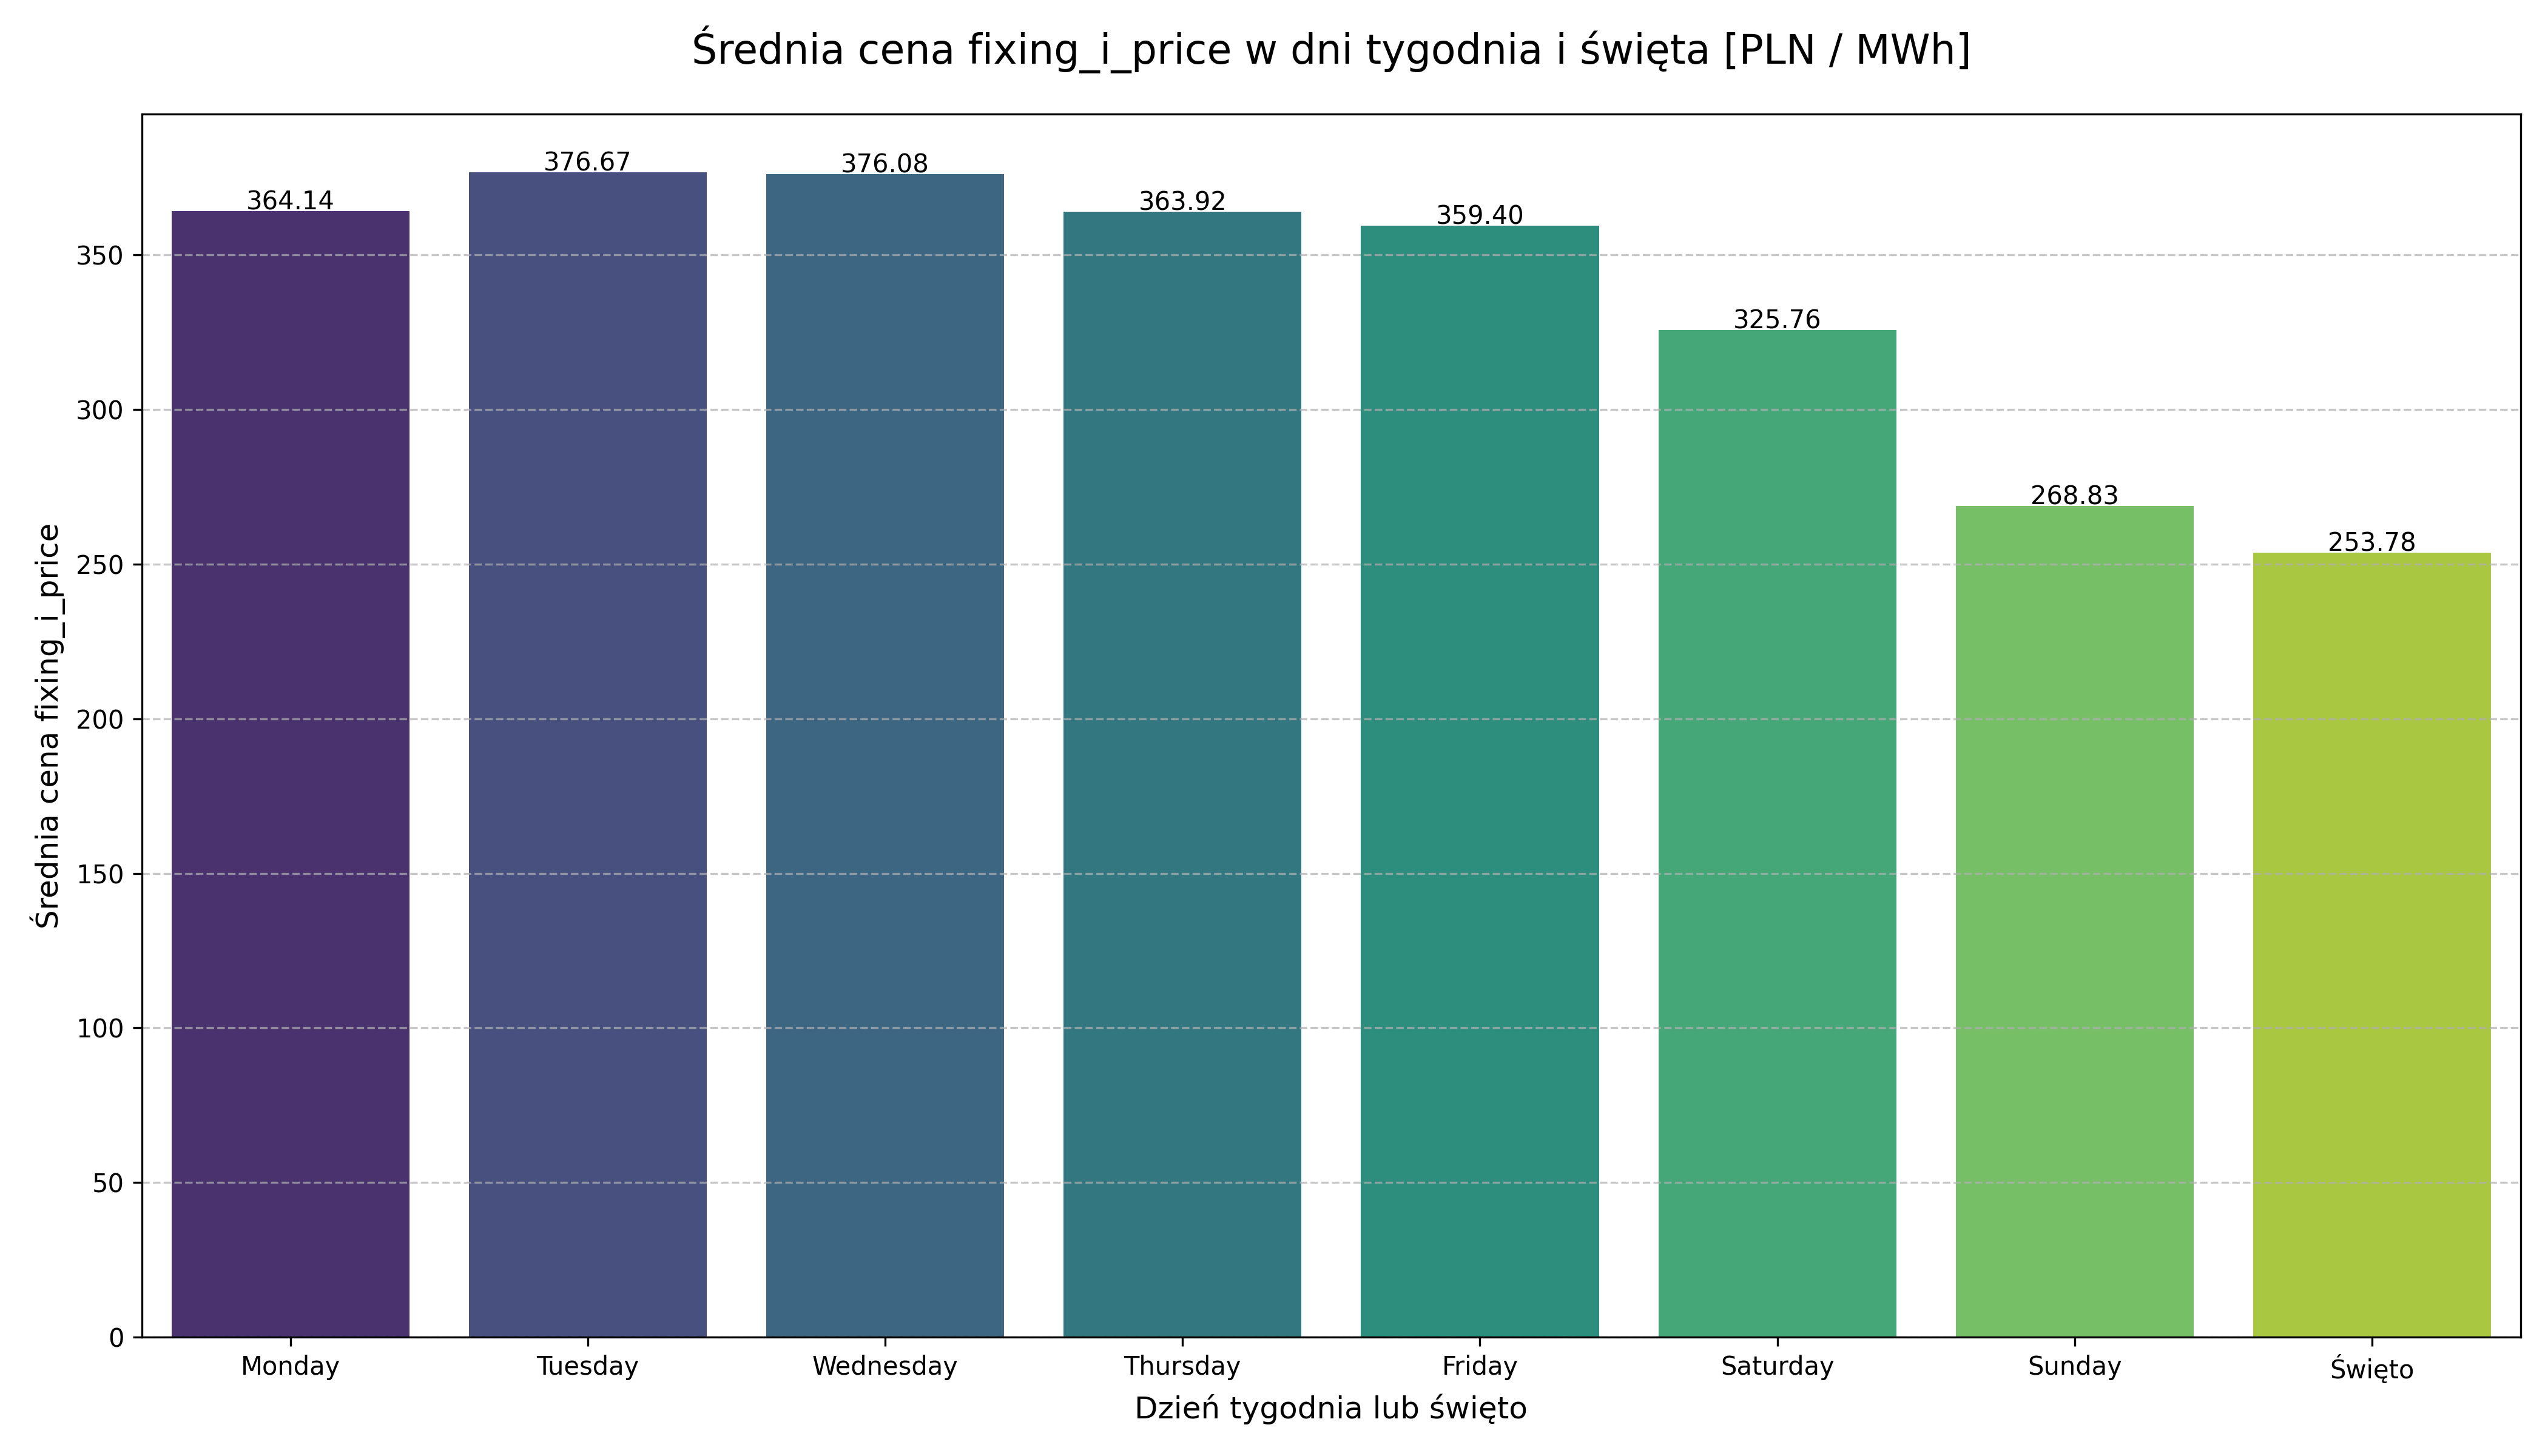
\includegraphics[width=0.9\textwidth]{../plots/fixing_i_price_weekdays_holidays.png}
    \caption{Korelacja dni tygodnia z cenami energii na RDN.}
    \label{fig:seasonal-correlation}
\end{figure}

Zmienna \texttt{day\_of\_week} reprezentuje dzień tygodnia (0--6, gdzie 0 to poniedziałek, a 6 to niedziela) i pozwala modelowi uwzględnić cykliczność tygodniową w cenach energii. Z wykresu wynika, że zapotrzebowanie na energię jest zazwyczaj wyższe w dni robocze, gdy działa przemysł i biura, a niższe w weekendy i święta, gdy aktywność gospodarcza jest mniejsza. Ta cykliczność przekłada się na ceny energii na RDN: w dni robocze ceny są zazwyczaj wyższe, szczególnie w godzinach szczytu. Wprowadzone zmienne sezonowe pozwalają modelowi lepiej uchwycić te wzorce, co jest istotne w zadaniu modelowania.

\subsubsection{Ceny historyczne}
\label{subsec:historical_prices}

Do wykresu 
Zmienne historyczne \texttt{fixing\_i\_price\_lag24} i \texttt{fixing\_i\_price\_lag168}, zostały wprowadzone do zbioru danych w celu uchwycenia autokorelacji w cenach energii na RDN. Zmienne te zostały wygenerowane na podstawie kolumny \texttt{fixing\_i\_price}, która reprezentuje cenę energii na RDN w danej godzinie (w PLN/MWh), poprzez przesunięcie wartości o odpowiednio dobę i tydzień.

Dla pierwszych rekordów w danych (pierwsze 24 godziny dla \texttt{fixing\_i\_price\_lag24} i pierwsze 168 godzin dla \texttt{fixing\_i\_price\_lag168}) brakujące wartości zostały skopiowane z ceny z tego dnia, z tego powodu pierwszy tydzień nie będzie analizowany jako zbiór testowy.

Wprowadzenie zmiennych historycznych do modelu pozwala lepiej uchwycić autokorelację i cykliczność w cenach energii, co jest kluczowe dla poprawy dokładności prognoz. Ceny historyczne są często jednymi z najważniejszych predyktorów w modelach prognozowania cen energii, szczególnie w modelach autoregresyjnych i modelach uczenia maszynowego.

\subsubsection{Kurs wymiany PLN/USD}
\label{subsec:pln_usd}

Zmienna \texttt{pln\_usd} reprezentuje kurs wymiany złotego polskiego względem dolara amerykańskiego (USD/PLN) w danej godzinie. Dane te zostały pozyskane z oficjalnej strony Narodowego Banku Polskiego (NBP) w granulacji dziennej. W celu dopasowania danych do godzinowego formatu RDN, wartości kursu zostały przypisane do wszystkich godzin w danym dniu. W przypadku dni wolnych od pracy lub braku dostępnych danych, wartości kursu zostały interpolowane.

\begin{table}[H]
    \centering
    \begin{tabular}{|c|c|}
    \hline
    \textbf{Rok} & \textbf{Średni kurs PLN/USD} \\ \hline
    2016 & 3.94 \\ \hline
    2017 & 3.78 \\ \hline
    2018 & 3.61 \\ \hline
    2019 & 3.84 \\ \hline
    2020 & 3.90 \\ \hline
    2021 & 3.86 \\ \hline
    2022 & 4.46 \\ \hline
    2023 & 4.20 \\ \hline
    2024 & 3.98 \\ \hline
    \end{tabular}
    \caption{Średni kurs wymiany PLN/USD w latach 2016--2024. Źródło: Opracowanie własne na podstawie danych NBP.}
    \label{tab:pln-usd-exchange-rate}
\end{table}

Kurs wymiany PLN/USD jest istotnym czynnikiem w kontekście prognozowania cen energii na RDN, ponieważ Polska importuje znaczną część paliw kopalnych, takich jak gaz ziemny i ropa naftowa, które są wyceniane w dolarach amerykańskich. Wzrost kursu PLN/USD (czyli osłabienie złotego względem dolara) zwiększa koszty importu tych paliw. Kurs polskiego złotego odzwierciedla też zmiany w gospodarce krajowej i globalnej. Próbując stabilizować kurs złotego, NBP zmienia politykę monetarną kraju, co może wpływać na ceny energii.
    \chapter{Eksploracja danych}
\label{sec:eksploracja}

W niniejszym rozdziale przedstawiono proces przygotowania omówionego zestawu danych. Proces eksploracji danych ubejmuje obsługę braków wartości, dostosowanie granulacji zmiennych, analizę korelacji, podział danych na okresy o różnej zmienności, podział na zbiory treningowy, walidacyjny i testowy oraz preprocessing danych przed modelowaniem.

\section{Wstępna obróbka danych}
\subsubsection{Obsługa braków wartości}
Pierwszym krokiem eksploracji jest analiza i obsługa brakujących wartości w zbiorze danych. Braki wartości w zmiennych objaśniających mogą wynikać z przyczyny, że w trakcie niektórych godzin pomiary nie były zbierane, lub z powodu błędów w danych, które mogły prowadzić do ich usunięcia. Na szczęście pierwotny zbiór danych zawierał niewiele braków i nie były one zbyt ciągłe w kontekście całego zbioru. W związku z tym rekordy zawierające brakujące wartości w miejscu dowolnej zmiennej zostały usunięte. Z oczekiwanych 78912 rekordów godzinowych pozostało 78451. Jest to zaledwie 0.55\% braków, co jest nie powinno stanowić problemu w dalszej analizie.

Niektóre zmienne, takie jak kursy walut czy ceny paliw kopalnych miały braki w okresach zamkniętego rynku, czyli weeekendy i święta. W takich przypadkach brakujące wartości zostały przeniesione z poprzedniego dnia handlu. 

\subsubsection{Obsługa granulacji}
Dane użyte w pracy charakteryzowały się różną granulacją czasową. PSE udostępnia dane dotyczące sieci energii elektrycznej, w tym handlu w rozdzielczości godzinowej. Zmienne pogodowe również mają granulację dzienną. Natomiast zmienne makroekonomiczne, takie jak ceny paliw, są dostępne w częstotliwości dniowej lub tygodniowej.

Aby ujednolicić granulację do poziomu godzinowego, zastosowano dwie techniki. W przypadku zmiennych o granulacji dziennej, takich jak dane pogodowe, założono, że wartości w ciągu doby nie ulegają zmianie. Wartości dzienne przypisano więc każdej godzinie danego dnia, co pozwoliło na zachowanie prostoty przy jednoczesnym dostosowaniu danych do godzinowej rozdzielczości ceny energii. 

Dla zmiennych o rzadszych granulacji, na przykład dla ceny węgla (miesięczna) oraz emisji CO2 (tygodniowa), przeprowadzono uzupełnianie danych metodą interpolacji liniowej między sąsiednimi wartościami. Poniższy przykład dla granulacji tygodniowej.
\[
\text{cena w dniu } d = \text{cena w tygodniu } t + \left( \frac{\text{cena w tygodniu } t+1 - \text{cena w tygodniu } t}{6} \right) \times d
\]
, gdzie \( \quad d \in [t, t+1] \) \newline
Następnie, podobnie jak w przypadku danych dziennych, wartości te przypisano każdej godzinie w danej dobie. Podejście to umożliwiło ujednolicenie wszystkich zmiennych do godzinowej rozdzielczości danych docelowych, co jest niezbędnym krokiem dla poddania zbioru danych analizie.

\section{Analiza korelacji}

Aby zbadać zależności między zmiennymi objaśniającymi a zmienną docelową, przeprowadzono analizę korelacji, wykorzystując dwa współczynniki: Pearsona i Spearmana. Wybór odpowiedniego współczynnika dla każdej zmiennej oparto na charakterze jej relacji z \texttt{fixing\_i\_price}, co pozwoliło na bardziej precyzyjne oszacowanie siły i rodzaju zależności.

Współczynnik korelacji Pearsona (\( r \)) mierzy liniową zależność między dwiema zmiennymi. Jest on zdefiniowany wzorem:
\[
r = \frac{\sum_{i=1}^{n} (x_i - \bar{x})(y_i - \bar{y})}{\sqrt{\sum_{i=1}^{n} (x_i - \bar{x})^2} \sqrt{\sum_{i=1}^{n} (y_i - \bar{y})^2}},
\]
gdzie \( x_i \) i \( y_i \) to wartości zmiennych i danej zmiennej objaśniającej), \( \bar{x} \) i \( \bar{y} \) to ich średnie, a \( n \) to liczba obserwacji. Współczynnik Pearsona przyjmuje wartości w przedziale \([-1, 1]\), gdzie \( r = 1 \) oznacza doskonałą dodatnią zależność liniową, \( r = -1 \) doskonałą ujemną zależność liniową, a \( r = 0 \) brak liniowej zależności.

Pearson jest odpowiedni dla zmiennych, których relacja jest liniowa. Na przykład wzrost zapotrzebowania zwykle większa ceny energii liniowo.

Współczynnik korelacji Spearmana (\( \rho \)) mierzy monotoniczną zależność między zmiennymi, co czyni go bardziej odpowiednim dla relacji nieliniowych. Spearman opiera się na rangach wartości zmiennych, a jego wzór to:

\[
\rho = 1 - \frac{6 \sum_{i=1}^{n} d_i^2}{n(n^2 - 1)},
\]

gdzie \( d_i \) to różnica między rangami wartości \( x_i \) i \( y_i \). Współczynnik Spearmana również przyjmuje wartości w przedziale \([-1, 1]\), ale nie zakłada liniowości relacji - wystarczy, że wzrost jednej zmiennej odpowiada wzrostowi (lub spadkowi) drugiej w sposób monotoniczny.

Spearman jest szczególnie użyteczny dla zmiennych o nieliniowej relacji z \texttt{fixing\_i\_price}. Na przykład wzrost cen gazu w 2022 roku prowadził do nieproporcjonalnego wzrostu cen energii, co lepiej oddaje Spearman niż Pearson.

W celu wyboru odpowiedniego współczynnika korelacji obliczono zarówno korelację Pearsona, jak i Spearmana dla wszystkich zmiennych objaśniających względem \texttt{fixing\_i\_price}. Następnie obliczono bezwzględną różnicę między tymi współczynnikami (\(| \rho - r |\)). Zmienne, dla których różnica była większa niż 0,1, uznano za posiadające nieliniową relację z \texttt{fixing\_i\_price}, stosując dla nich korelację Spearmana. W pozostałych przypadkach wybrano korelację Pearsona, zakładając liniową zależność. 

Analiza wykazała, że zmienne takie jak \texttt{co2\_price} (różnica 0,114), \texttt{coal\_pscmi1\_pln\_per\_gj} (0,161), \texttt{pln\_usd} (0,112), \texttt{solar} (0,172), \texttt{gas} (0,153), \texttt{biomass} (0,174), \texttt{coal-derived} (0,142) oraz zmienne związane z promieniowaniem słonecznym (różnice 0,106-0,115) mają nieliniową relację z \texttt{fixing\_i\_price}. Nieliniowość wynika z charakteru tych zmiennych - na przykład wysoka produkcja energii z fotowoltaiki w miesiącach letnich obniża ceny energii w sposób nieproporcjonalny, co prowadzi do bardzo niskich, a czasem ujemnych cen. Podobnie gwałtowny wzrost cen CO2 w okresie niespokojnym (2020-2023) zwiększał koszty produkcji energii w elektrowniach węglowych, ale efekt ten był wzmacniany przez inne czynniki, takie jak spekulacje rynkowe.

W wyniku tego powstał następujący wykres korelacji poniżej

\begin{figure}[H]
    \centering
    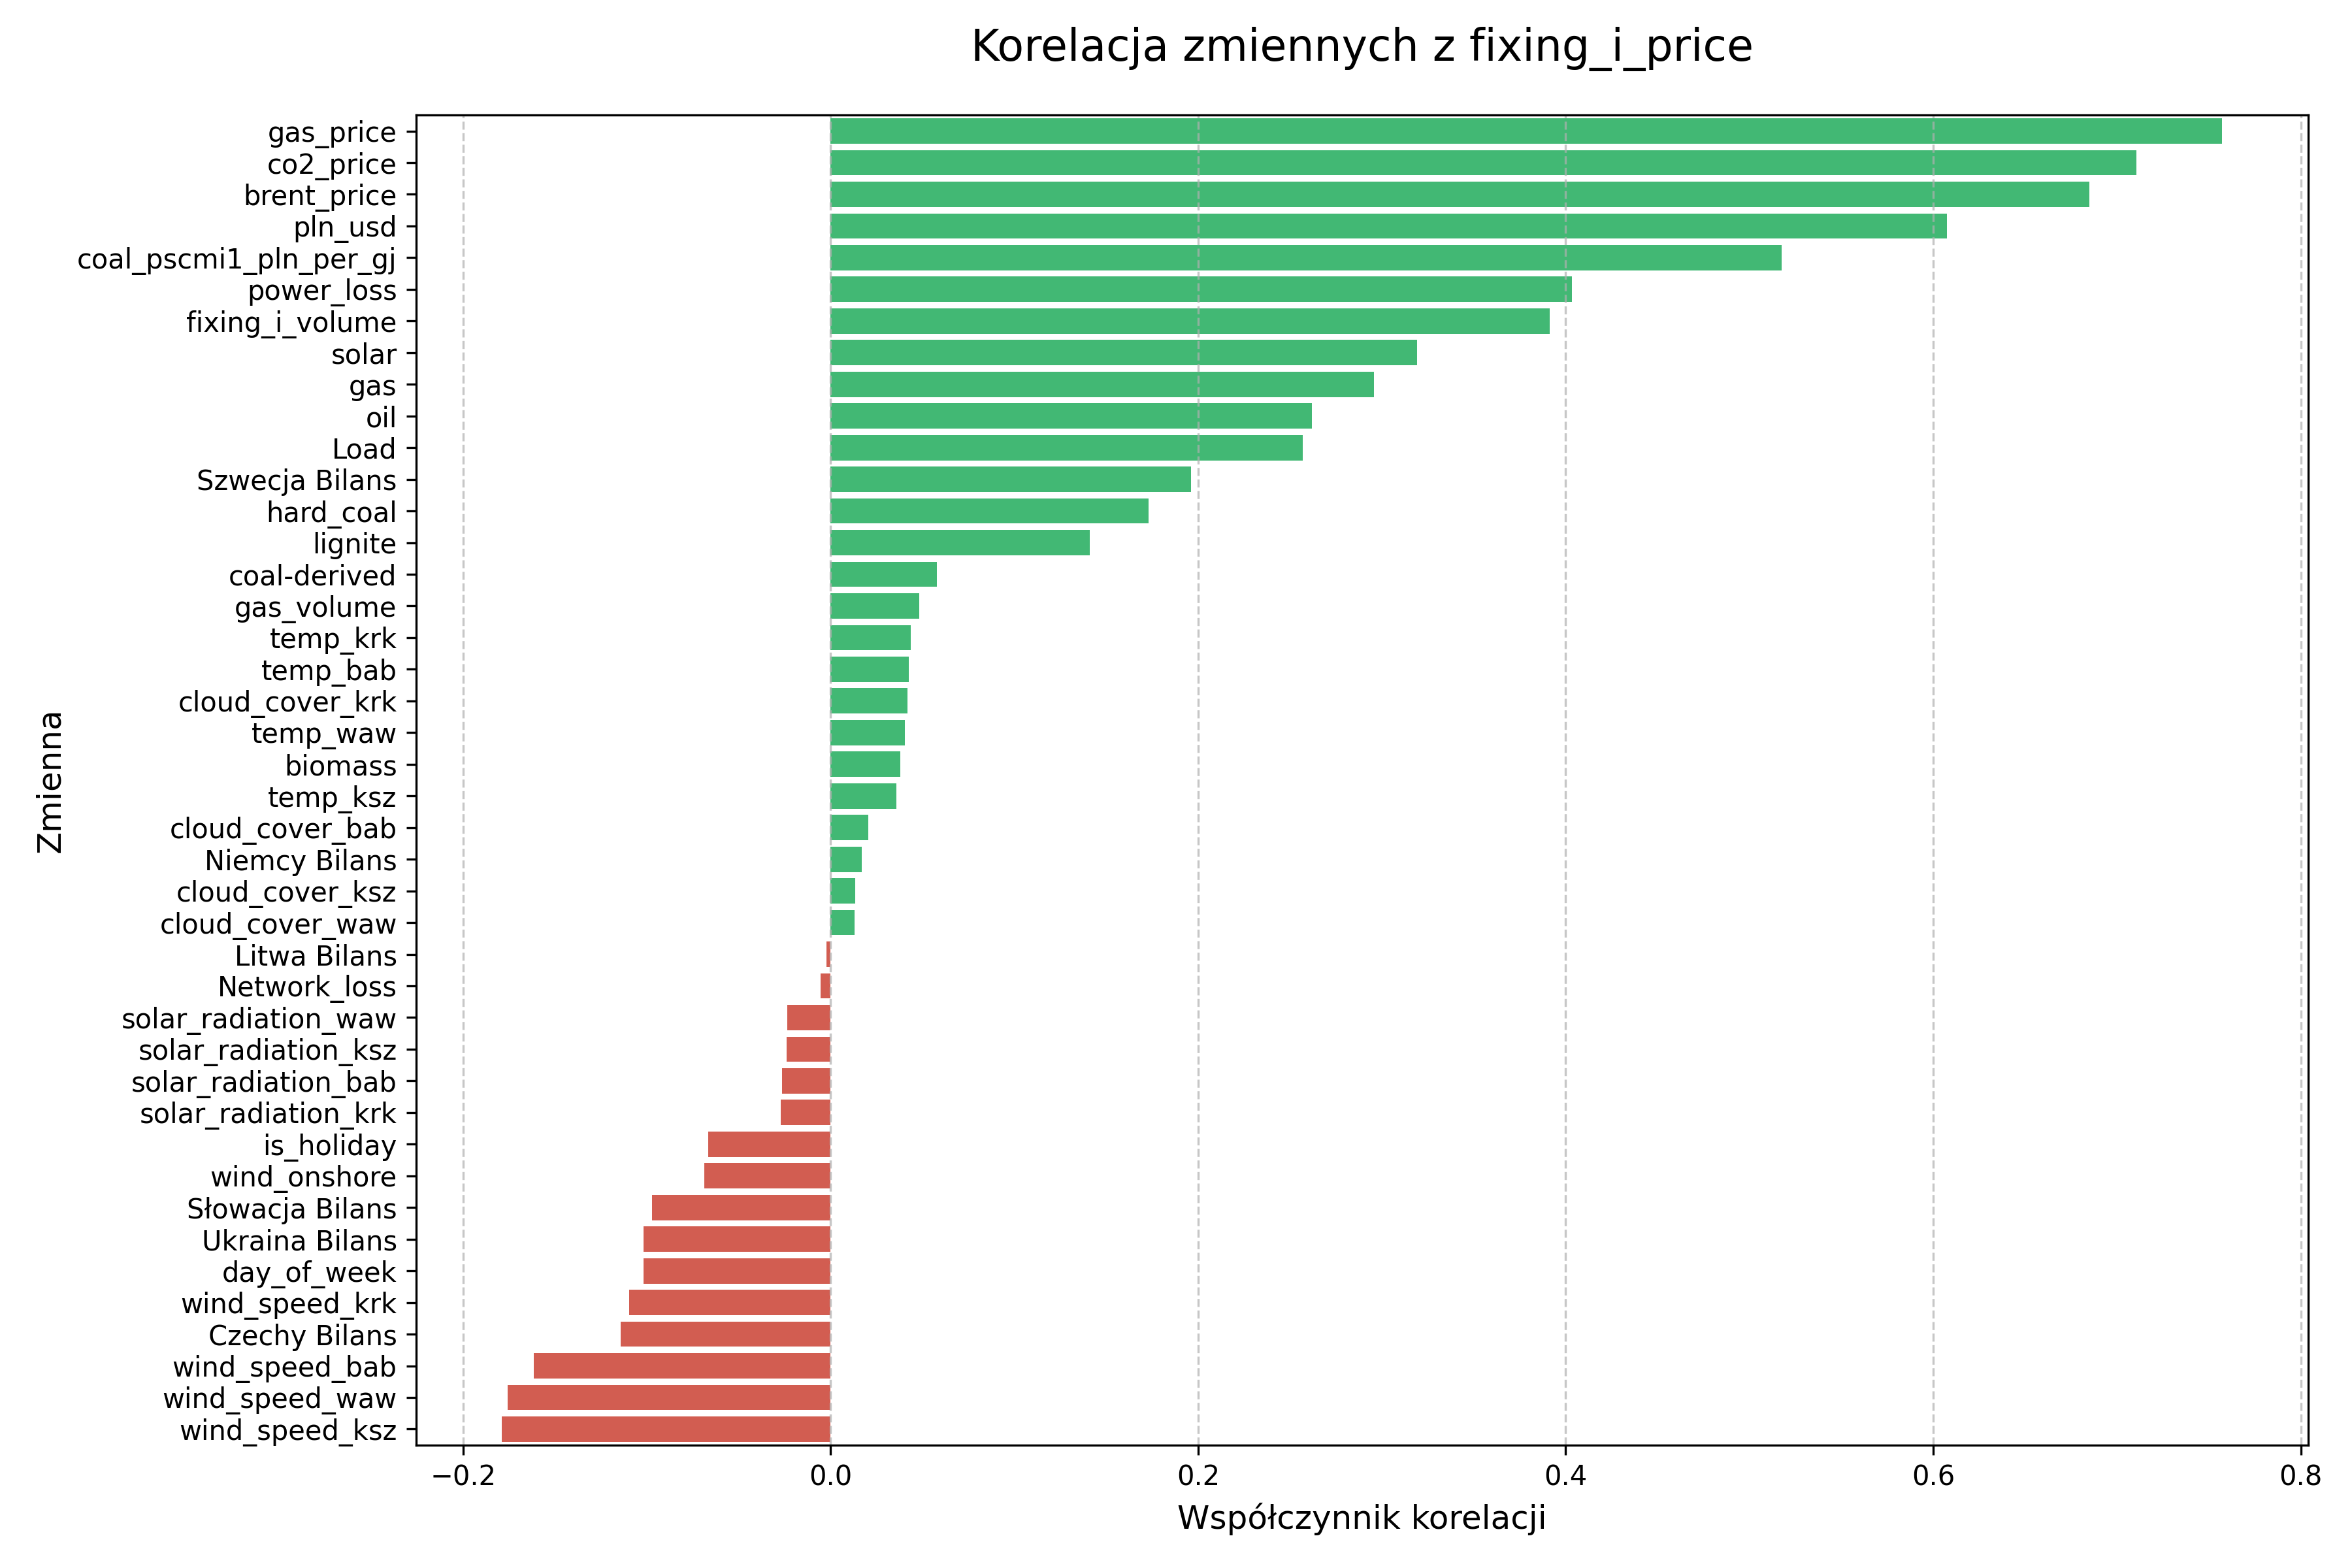
\includegraphics[width=0.9\textwidth]{../plots/correlation_with_fixing_i_price.png}
    \caption{Wykres korelacji zmiennych objaśniających względem zmiennej docelowej \texttt{fixing\_i\_price}.}
    \label{fig:correlation_plot}
\end{figure}

Zgodnie z literaturą, największy wpływ na ceny energii mają zmienne, które powstały w wyniku przetworzenia zmiennej objaśnianej, czyli ceny opóźnione i średnie. Koljenymi zmiennymi wykazującymi silną korelację są ceny na surowce, kurs pollskiego złotego oraz zapotrzebowanie i wolumen. Sprzeczna z logiką może być pozytywna korelacja ceny z zmienną \texttt{solar}, która wskazuje na produkcję energii z paneli fotowoltaicznych. Wynika to prawdopodobnie z faktu, w momentach, gdy świeci słońce i produkcja energii z OZE jest wysoka, zapotrzebowanie również jest zwiększone i to powoduje wzrost cen. Z kolei wartości reprezentujące parametry pogodowe nie wykazują istotnej korelacji. 

Produkcja energii z odnawialnych źródeł i gazu również odgrywa rolę. Zmienna \texttt{solar} (Spearman: 0,490) wskazuje, że wysoka produkcja energii z fotowoltaiki obniża ceny energii, szczególnie w miesiącach letnich, gdzie nadpodaż energii z OZE może prowadzić do bardzo niskich cen. \texttt{gas} (Spearman: 0,449) pokazuje, że produkcja energii z gazu ma nieliniowy wpływ, zależny od cen gazu i dostępności innych źródeł energii. Ponadto zmienne takie jak \texttt{fixing\_i\_volume} (Spearman: 0,442), \texttt{power\_loss} (Spearman: 0,441), \texttt{oil} (Spearman: 0,349) oraz \texttt{Load} (Pearson: 0,256) mają umiarkowany wpływ, odzwierciedlając znaczenie wolumenu obrotu, strat w sieci, produkcji z oleju oraz zapotrzebowania na energię.

\subsubsection{Zbiór danych skrócony}
\label{sec:shortened_dataset}
Na podstawie analizy korelacji stworzony został skrócony zbiór danych, który z pierwotnych 54 regresorów zostawia najbardziej istotne. Tymi zmiennymi zostały wszystkie przekraczające próg istotności na poziomie \texttt{0.2},  zmienne sezonowe określające dzień tygodnia, miesiąc, godzinę oraz święta, średnia arytmetyczna ze zmiennych objaśniających prędkość wiatru w Polsce, gdyż wykazują one najmocniejszą odwrotną korelację oraz zmienna objaśniająca generację OZE w procentach, ponieważ jest to ważna zmienna z punktu widzenia literatury. W wyniku tego powstał zbiór danych z 27 zmiennymi objaśniającymi. Taki zbiór danych został określony jako \texttt{zbiór danych skrócony} i będzie użyty w dalszej części pracy do analizy w celu sprawdzenia istotności zbioru danych o największej ilości parametrów. Poniżej przedstawiono mapę cieplną dla zmiennych objaśniających w zbiorze danych skróconym bez uwzględnienia zmiennych opóźnioncyh i średnich. 

\begin{figure}[H]
    \centering
    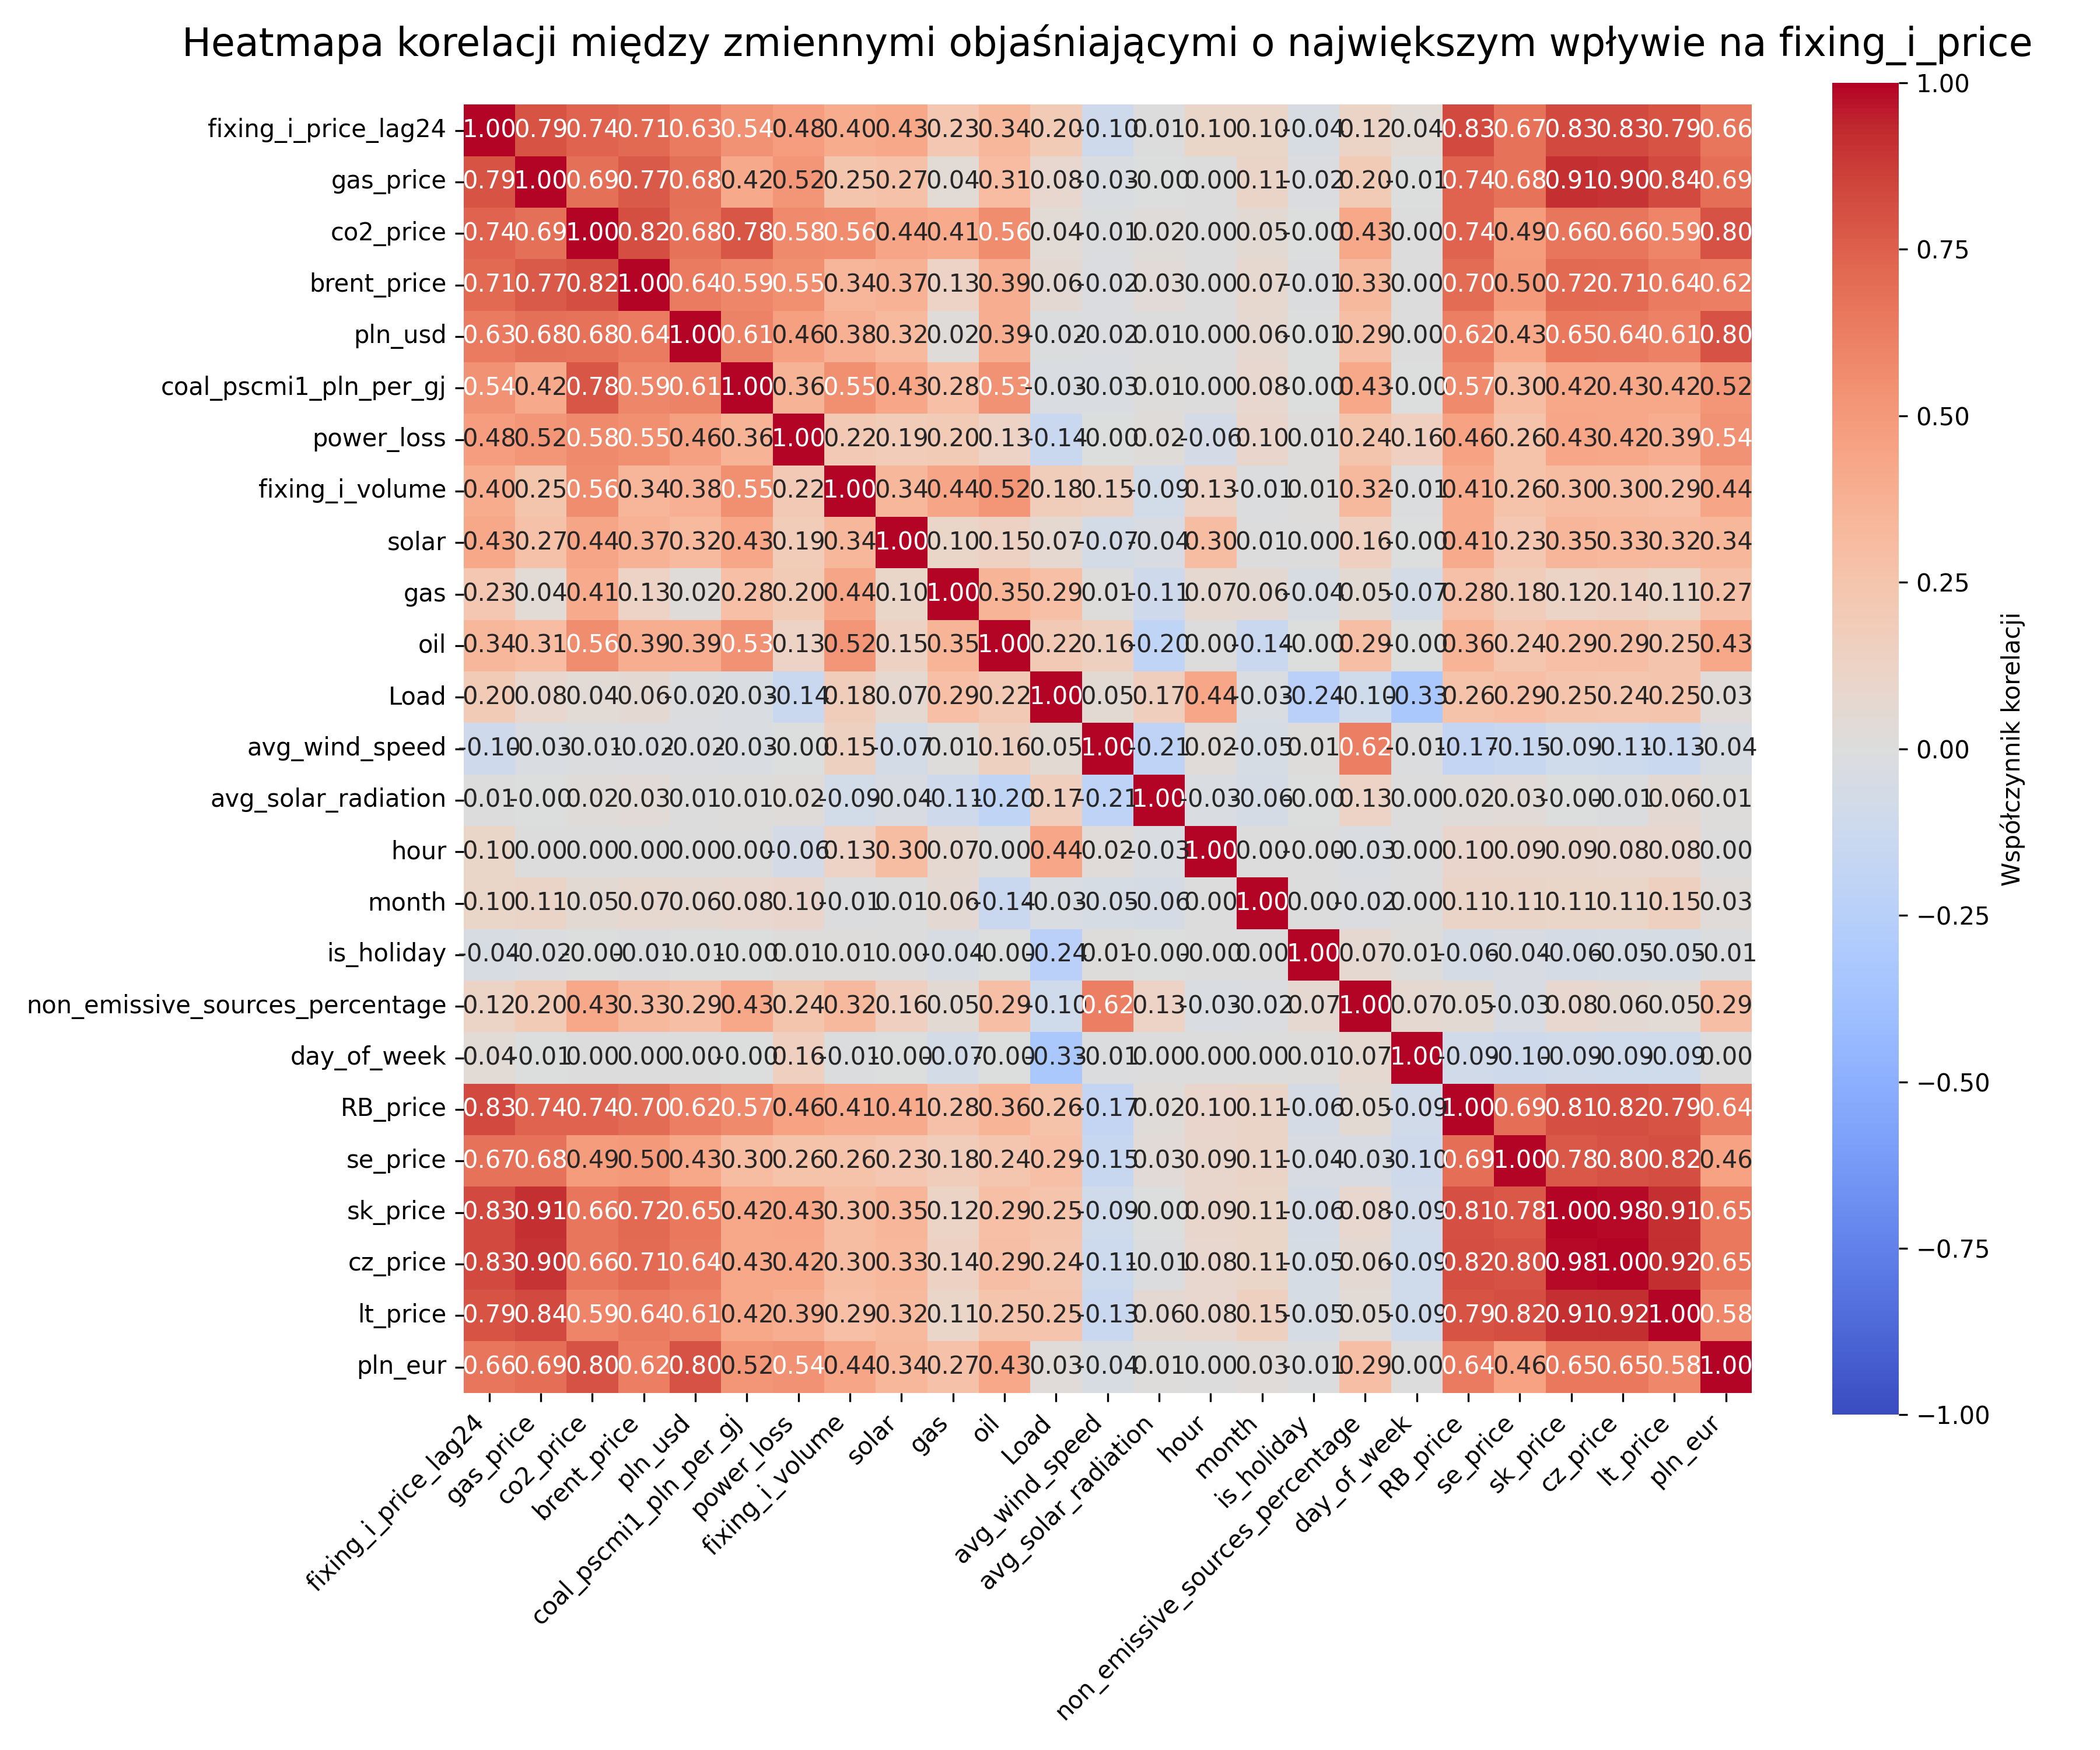
\includegraphics[width=0.9\textwidth]{../plots/heatmap_short_db_features.png}
    \caption{Mapa cieplna korelacji zmiennych objaśniających w skróconym zbiorze danych.}
    \label{fig:heatmap_shortened_dataset}
\end{figure}

Z powyższej mapy cieplnej wynika, że zmienne o największej korelacji z ceną energii w dużym stopniu są również skorelowane pomiędzy sobą. 

\section{Podział danych}

\subsubsection{Podział na okresy spokojny i niespokojny}

Dane zostały podzielone na dwa okresy w celu uwzględnienia różnych warunków rynkowych i ich wpływu na ceny energii. Okres spokojny (2016-2019) charakteryzuje się stabilnymi cenami energii, wynikającymi z braku znaczących szoków podażowych, łatwiej przewidywalnych cen paliw oraz łagodnego wzrostu cen CO2 w ramach polityki klimatycznej UE. W tym okresie nie występowały większe kryzysy geopolityczne ani pandemie, co pozwoliło na utrzymanie cen w stosunkowo wąskim zakresie.

Okres niespokojny (2020-2023) został zdominowany przez szereg wydarzeń, które drastycznie wpłynęły na rynek energii. Pandemia COVID-19 w latach 2020-2021 początkowo obniżyła zapotrzebowanie na energię, ale ożywienie gospodarcze w 2021 roku spowodowało gwałtowny wzrost cen. Kryzys energetyczny w latach 2021-2022, związany z ograniczoną podażą gazu, rekordowymi cenami CO2 oraz wysokimi cenami węgla, doprowadził do ekstremalnych skoków cen energii. Wybuch wojny na Ukrainie w 2022 roku dodatkowo zaostrzył sytuację, powodując przerwanie dostaw gazu z Rosji, sankcje i spekulacje rynkowe, co przełożyło się na rekordowe ceny energii. W tym okresie pojawiły się również ujemne ceny, wynikające z nadpodaży energii z OZE i ograniczonej elastyczności systemu elektroenergetycznego.

Statystyki opisowe dla obu okresów przedstawiono w tabeli~\ref{tab:periods_stats_comparison}. Okres spokojny charakteryzuje się niższą średnią ceną, mniejszą zmiennością i dużo mniejszym odchyleniem standardowym, co odzwierciedla stosunkowo stabilne warunki rynkowe. W okresie niespokojnym średnia cena wzrosła, a współczynnik zmienności i odchylenie znacząco rosną. W latach 2020-2023 pojawiły się również ujemne ceny oraz rekordowe maksima. Podział na te dwa okresy i poddanie ich osobnej analizie pozwoli lepiej ocenić skuteczność wybranych cech i modeli w różnych warunkach rynkowych.

\begin{table}[h]
    \centering
    \caption{Porównanie statystyk opisowych cen energii w okresach spokojnym (2016-2019) i niespokojnym (2020-2023).}
    \label{tab:periods_stats_comparison}
    \begin{tabular}{|l|c|c|}
        \hline
        \textbf{Miara} & \textbf{Okres spokojny} & \textbf{Okres niespokojny} \\
        \hline
        Średnia (PLN/MWh) & 193,51 & 478,06 \\
        \hline
        Mediana (PLN/MWh) & 182,00 & 412,00 \\
        \hline
        Odchylenie standardowe (PLN/MWh) & 70,67 & 321,39 \\
        \hline
        Współczynnik zmienności (\%) & 36,52 & 67,23 \\
        \hline
        Kwartyl Q1 (25\%) (PLN/MWh) & 143,66 & 246,41 \\
        \hline
        Kwartyl Q3 (75\%) (PLN/MWh) & 229,35 & 609,00 \\
        \hline
        Minimum (PLN/MWh) & 31,00 & -50,00 \\
        \hline
        Maksimum (PLN/MWh) & 1199,53 & 3812,45 \\
        \hline
        Procent dni z ceną powyżej 500 PLN/MWh (\%) & 0,41 & 36,94 \\
        \hline
    \end{tabular}
\end{table}

\subsubsection{Podział danych na zbiory treningowe i testowe}

Dane zostały podzielone na zbiory treningowe i testowe w obrębie każdego z dwóch okresów, aby uwzględnić strukturę szeregów czasowych. Podział został przeprowadzony sekwencyjnie w proporcji 75/25, co zapewnia dużą ilość danych do treningu (3 lata) oraz odpowiednią ilość danych do testowania (1 rok). W przypadku takiego podziału w zbiorach testowych można przetestować wszystkie okresy sezonowe.

\begin{figure}[h]
    \centering
    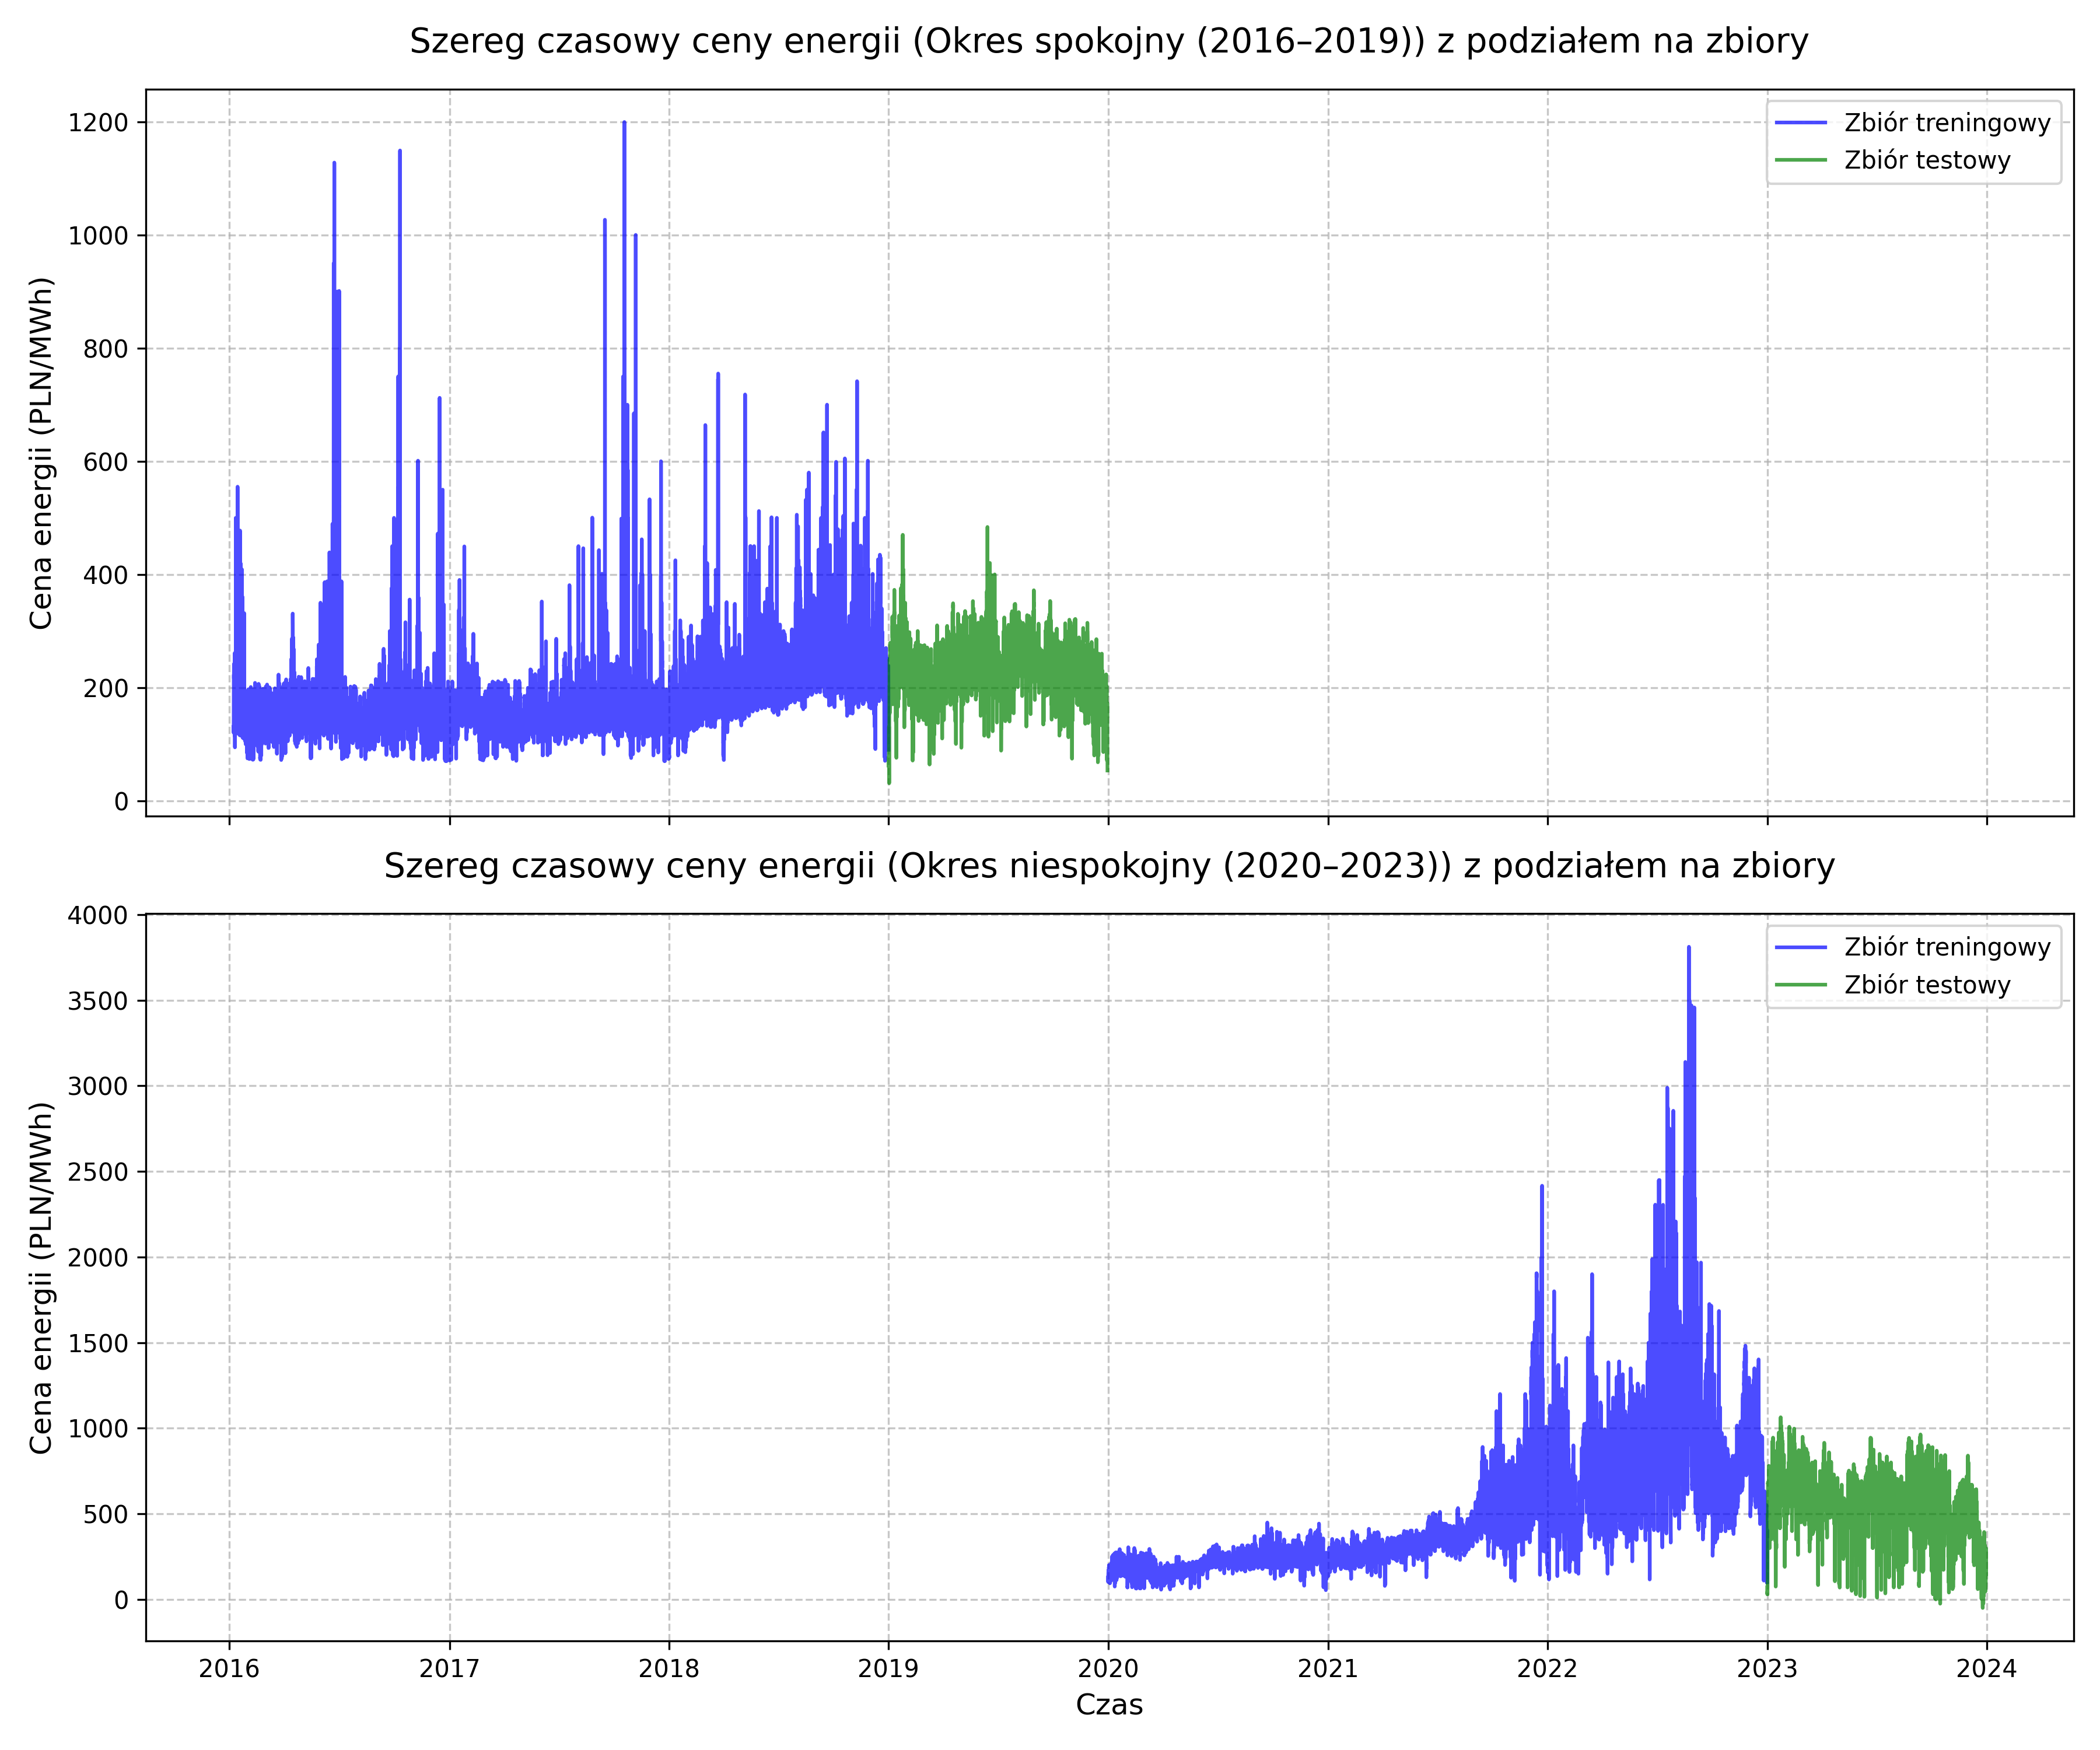
\includegraphics[width=0.9\textwidth]{../../plots/periods_split_combined.png}
    \caption{Podział szeregów czasowych cen energii na zbiory treningowe i testowe}
    \label{fig:periods_split_combined}
\end{figure}

\section{Przygotowanie danych}

Przed przystąpieniem do modelowania dane zostały poddane szeregu kroków preprocessingu, aby zapewnić ich odpowiednią jakość i format dla wybranych modeli.

Pierwszym krokiem jest kodowanie zmiennych cyklicznych. Zmienne sezonowe mają charakter cykliczny (np. po godzinie 23 następuje 0, po grudniu następuje styczeń). Aby uwzględnić tę cykliczność, zastosowano kodowanie za pomocą funkcji sinusoidalnych:

\begin{itemize}
    \item Dla \texttt{day\_of\_week}: \(\sin\left(\frac{2\pi \cdot \text{day\_of\_week}}{7}\right)\),
    \item Dla \texttt{month}: \(\sin\left(\frac{2\pi \cdot \text{month}}{12}\right)\),
    \item Dla \texttt{hour}: \(\sin\left(\frac{2\pi \cdot \text{hour}}{24}\right)\).
\end{itemize}

Oryginalne zmienne zostały usunięte, a ich zakodowane wersje dodano do zbioru danych. Kodowanie sinusoidalne pozwala modelom lepiej uchwycić cykliczność danych, w przeciwieństwie do kodowania typu one-hot, które zwiększyłoby wymiarowość danych i nie uwzględniało cykliczności.

Następnie, wszystkie zmienne numeryczne niebinarne zostały poddane standaryzacji StandardScaler z biblioteki \texttt{sklearn}. Standaryzacja polega na przekształceniu zmiennych, aby miały średnią 0 i odchylenie standardowe 1. Wartości zmiennych zostały przekształcone według wzoru:
\[ z = \frac{x - \mu}{\sigma}, \]
gdzie \( z \) to wartość po standaryzacji, \( x \) to wartość przed standaryzacją, \( \mu \) to średnia zmiennej, a \( \sigma \) to odchylenie standardowe. 

Standaryzacja jest kluczowym krokiem w preprocessingu danych, ponieważ większość algorytmów uczenia maszynowego zakłada, że dane mają podobną skalę. W przeciwnym razie algorytmy mogą być wrażliwe na różnice w skali zmiennych, co prowadzi do nieoptymalnych wyników. Proces standaryzacji został przeprowadzony osobno dla każdego z okresów spokojnego i niespokojnego osobno, aby uwzględnić różnice w rozkładach danych między tymi okresami. W obrębie każdego okresu parametry standaryzacji (średnia i odchylenie standardowe) obliczono na zbiorze treningowym i zastosowano zarówno do danych treningowych, jak i testowych, aby uniknąć wycieku informacji.

Wartości odstające (np. ekstremalnie wysokie ceny w okresie niespokojnym, takie jak 3812,45 PLN/MWh) nie zostały zmodyfikowane, ponieważ odzwierciedlają rzeczywiste zjawiska rynkowe (np. kryzys energetyczny w 2022 roku). Ich wpływ na modele będzie monitorowany podczas analizy wyników.

    \chapter{Metodologia}
\label{ch:metodologia}

W rozdziale tym przedstawiono metodologię przeprowadzonych badań. Rozdział składa się z dwóch sekcji. W pierwszej przedstawiono metodykę oceny jakości prognoz, a w drugiej omówiono metodykę prognozowania cen energii elektrycznej.

\section{Ocena jakości prognoz}
\label{sec:ocena_jakosci_prognoz}

Ocena jakości modeli prognozowania cen energii elektrycznej jest kluczowym etapem analizy, ponieważ pozwala na porównanie skuteczności różnych podejść. W niniejszej pracy zastosowano następujące popularne metryki oceny: Mean Absolute Error (MAE), Root Mean Squared Error (RMSE), Mean Absolute Percentage Error (MAPE), Symmetric Mean Absolute Percentage Error (sMAPE) oraz \( R^2 \). Wszystkie z tych metryk są omawiane w literaturze porównania skuteczności modeli \cite{en17225797}. W pracy prof. Werona \cite{WERON20141030} podano, że nie ma standardu obliczenia metryk EPF i wspomina o innych metrykach stosowanych przez innych autorów artykułów, między innymi wymieniono -- Ważony Średni Błąd Bezwzględny (WMAE), średni błąd dniowy (MDE) i tygodniowy (MWE). Niemniej jednak, w tej pracy skupiono się na tych najszerzej stosowanych metrykach. Każda z tych metryk ma swoje zalety i ograniczenia, których omówienie jest przedstawione poniżej, wraz z ich matematycznymi definicjami i przykładami zastosowania w EPF.

\subsection{Mean Absolute Error (MAE)}
\label{subsec:mae}

Mean Absolute Error jest jedną z najprostszych i najczęściej stosowanych metryk w prognozowaniu szeregów czasowych, w tym w EPF. MAE mierzy średnią wartość bezwzględnych błędów prognoz, co pozwala na ocenę dokładności modelu bez uwzględniania kierunku błędu (nad- lub niedoszacowania).

Matematyczna definicja MAE jest następująca:

\[
\text{MAE} = \frac{1}{n} \sum_{t=1}^{n} \left| y_t - \hat{y}_t \right|
\]

gdzie:
\begin{itemize}
    \item \( y_t \) to rzeczywista cena energii w godzinie \( t \),
    \item \( \hat{y}_t \) to przewidywana cena energii w godzinie \( t \),
    \item \( n \) to liczba obserwacji w zbiorze testowym.
\end{itemize}

MAE jest wyrażane w tej samej jednostce co prognozowane wartości (w omawianym przypadku jest to PLN/MWh), co czyni je łatwym do interpretacji. Na przykład, jeśli MAE wynosi 10 PLN/MWh, oznacza to, że średni błąd prognozy wynosi 10 PLN na każdą megawatogodzinę.

\textbf{Zalety MAE:}
\begin{itemize}
    \item Prosta interpretacja i obliczenia.
    \item Równomierne traktowanie wszystkich błędów, niezależnie od ich kierunku.
\end{itemize}

\textbf{Ograniczenia MAE:}
\begin{itemize}
    \item Nie uwzględnia kwadratu błędów, przez co nie penalizuje większych odchyleń w sposób szczególny, co może być problematyczne w EPF, gdzie duże skoki cen (np. w godzinach szczytu) są istotne.
\end{itemize}

\subsection{Root Mean Squared Error (RMSE)}
\label{subsec:rmse}

Root Mean Squared Error (RMSE) jest kolejną popularną metryką w EPF, która uwzględnia kwadrat błędów, co powoduje większe uwzględnienie większych odchyleń między wartościami rzeczywistymi a przewidywanymi. RMSE jest szczególnie użyteczne w sytuacjach, gdzie duże błędy prognoz mogą mieć poważne konsekwencje ekonomiczne.

Definicja RMSE jest następująca:

\[
\text{RMSE} = \sqrt{\frac{1}{n} \sum_{t=1}^{n} \left( y_t - \hat{y}_t \right)^2}
\]

gdzie:
\begin{itemize}
    \item \( y_t \), \( \hat{y}_t \) i \( n \) mają takie same znaczenie jak w MAE.
\end{itemize}

RMSE jest również wyrażane w jednostkach oryginalnych danych, co ułatwia interpretację. Na przykład, RMSE równe 15 PLN/MWh oznacza, że typowy błąd prognozy (w sensie średniego kwadratu) wynosi 15 PLN na megawatogodzinę.

\textbf{Zalety RMSE:}
\begin{itemize}
    \item Większa wrażliwość na duże błędy, co jest istotne w EPF, gdzie skoki cen mogą być kosztowne.
\end{itemize}

\textbf{Ograniczenia RMSE:}
\begin{itemize}
    \item Wrażliwość na wartości odstające -- pojedyncze duże błędy mogą znacząco zawyżyć wartość RMSE.
    \item Mniej intuicyjne w interpretacji niż MAE, ponieważ kwadrat błędów zmienia skalę.
\end{itemize}

\subsection{Mean Absolute Percentage Error (MAPE)}
\label{subsec:mape}

Mean Absolute Percentage Error (MAPE) jest metryką wyrażającą błąd prognozy jako procent rzeczywistej wartości, co czyni ją szczególnie użyteczną w porównaniach między różnymi zbiorami danych lub rynkami o różnych poziomach cen.

Definicja MAPE jest następująca:

\[
\text{MAPE} = \frac{1}{n} \sum_{t=1}^{n} \left| \frac{y_t - \hat{y}_t}{y_t} \right| \times 100
\]

gdzie:
\begin{itemize}
    \item \( y_t \), \( \hat{y}_t \) i \( n \) mają takie same znaczenie jak wcześniej.
\end{itemize}

MAPE jest wyrażane w procentach, co ułatwia interpretację. Na przykład, MAPE równe 5\% oznacza, że średni błąd prognozy wynosi 5\% rzeczywistej ceny. W kontekście RDN, jeśli cena energii wynosi 200 PLN/MWh, a MAPE wynosi 5\%, średni błąd wynosi 10 PLN/MWh.

\textbf{Zalety MAPE:}
\begin{itemize}
    \item Intuicyjna interpretacja w procentach, nie trzeba zastanawiać się nad jednostkami bądź kursami walutowymi.
\end{itemize}

\textbf{Ograniczenia MAPE:}
\begin{itemize}
    \item Problemy z wartościami bliskimi zera -- jeśli \( y_t \) jest bardzo małe, co jest możliwe w godzinach nocnych, dzielenie przez \( y_t \) prowadzi do bardzo dużych wartości procentowych, a nawet do błędu matematycznego (dzielenie przez zero).
    \item Asymetria -- MAPE bardziej penalizuje niedoszacowania niż przeszacowania, co może prowadzić do nieobiektywnej oceny.
\end{itemize}

\subsection{Symmetric Mean Absolute Percentage Error (sMAPE)}
\label{subsec:smape}

Symmetric Mean Absolute Percentage Error (sMAPE) jest zmodyfikowaną wersją MAPE, która rozwiązuje problem asymetrii i dzielenia przez zero. sMAPE uwzględnia zarówno rzeczywiste, jak i przewidywane wartości w mianowniku, co czyni ją bardziej stabilną w sytuacjach, gdy ceny energii są niskie.

Definicja sMAPE jest następująca:

\[
\text{sMAPE} = \frac{1}{n} \sum_{t=1}^{n} \frac{\left| y_t - \hat{y}_t \right|}{\left( \left| y_t \right| + \left| \hat{y}_t \right| \right) / 2} \times 100
\]

gdzie:
\begin{itemize}
    \item \( y_t \), \( \hat{y}_t \) i \( n \) mają takie same znaczenie jak wcześniej.
\end{itemize}

Podobnie jak MAPE, sMAPE jest wyrażane w procentach. Na przykład, sMAPE równe 4\% oznacza, że średni błąd symetryczny wynosi 4\% średniej wartości rzeczywistej i przewidywanej ceny.

\textbf{Zalety sMAPE:}
\begin{itemize}
    \item Rozwiązuje problem dzielenia przez zero, co jest istotne w EPF, gdzie ceny mogą być bliskie zera.
    \item Symetria -- traktuje nad- i niedoszacowania w bardziej zrównoważony sposób niż MAPE.
\end{itemize}

\textbf{Ograniczenia sMAPE:}
\begin{itemize}
    \item Nadal może być wrażliwe na skrajne wartości, choć w mniejszym stopniu niż MAPE.
    \item Interpretacja jest mniej intuicyjna niż w przypadku MAE czy RMSE, ponieważ uwzględnia zarówno \( y_t \), jak i \( \hat{y}_t \) w mianowniku.
\end{itemize}

\subsection{Współczynnik determinacji}
\label{subsec:r2}

Współczynnik determinacji, oznaczany jako \( R^2 \), jest metryką powszechnie stosowaną w analizie regresji i prognozowaniu. \( R^2 \) mierzy, jak dobrze model wyjaśnia zmienność danych rzeczywistych, czyli jaki procent wariancji zmiennej zależnej jest wyjaśniony przez model prognostyczny. Jest to metryka szczególnie użyteczna w ocenie modeli liniowych, ale znajduje zastosowanie również w bardziej złożonych modelach, w celu ogólnej oceny ich dopasowania do danych.

Definicja \( R^2 \) jest następująca:

\[
R^2 = 1 - \frac{\sum_{t=1}^{n} \left( y_t - \hat{y}_t \right)^2}{\sum_{t=1}^{n} \left( y_t - \bar{y} \right)^2}
\]

gdzie:
\begin{itemize}
    \item \( y_t \), \( \hat{y}_t \) i \( n \) mają takie same znaczenie jak wcześniej,
    \item \( n \) to liczba obserwacji w zbiorze testowym.
\end{itemize}

Licznik w wyrażeniu \( \sum_{t=1}^{n} \left( y_t - \hat{y}_t \right)^2 \) to suma kwadratów reszt, czyli całkowity błąd modelu, natomiast mianownik \( \sum_{t=1}^{n} \left( y_t - \bar{y} \right)^2 \) to całkowita suma kwadratów, czyli całkowita wariancja danych względem ich średniej. \( R^2 \) przyjmuje wartości w przedziale od 0 do 1, gdzie:
\begin{itemize}
    \item \( R^2 = 1 \) oznacza, że model idealnie przewiduje wszystkie wartości (błąd wynosi 0),
    \item \( R^2 = 0 \) oznacza, że model nie wyjaśnia żadnej zmienności danych i jest równoważny prostemu modelowi średniej (\( \hat{y}_t = \bar{y} \)).
\end{itemize}

W kontekście EPF, na przykład na RDN, \( R^2 \) równe 0,85 oznaczałoby, że model wyjaśnia 85\% zmienności cen energii.

\textbf{Zalety \( R^2 \):}
\begin{itemize}
    \item Intuicyjna interpretacja -- \( R^2 \) jasno wskazuje, jaki procent zmienności danych jest wyjaśniony przez model.
    \item Bez jednostek -- umożliwia porównanie modeli na różnych zbiorach danych, niezależnie od skali cen (np. PLN/MWh na RDN vs. EUR/MWh na EEX).
\end{itemize}

\textbf{Ograniczenia \( R^2 \):}
\begin{itemize}
    \item Wrażliwość na przeuczenie -- \( R^2 \) może być zawyżone w modelach o dużej liczbie parametrów, szczególnie w przypadku małych zbiorów danych, co może prowadzić do mylnego wniosku o dobrym dopasowaniu modelu.
    \item Brak informacji o kierunku błędów -- \( R^2 \) nie rozróżnia, czy model nad- czy niedoszacowuje wartości, co w EPF może być istotne z ekonomicznego punktu widzenia.
\end{itemize}

W niniejszej pracy \( R^2 \) zostanie wykorzystane jako dodatkowa metryka oceny, aby uzupełnić analizę opartą na MAE, RMSE, MAPE, sMAPE.

\section{Wybrane metody weryfikacji zbioru danych}
\label{sec:metody_weryfikacji_zbioru_danych}

Stworzony zbiór danych z cechami objaśniającymi ceny energii elektrycznej należy zweryfikować pod kątem jego skuteczności. W związku z tym zostały wybrane cztery metody prognozowania.

\subsection{Regresja liniowa}

\textbf{Opis metody} \\
Regresja liniowa jest jednym z najprostszych i najczęściej stosowanych modeli statystycznych w analizie zbiorów danych. Zakłada liniową zależność między zmienną zależną, a zestawem zmiennych niezależnych (predyktorów). W kontekście EPF regresja liniowa jest często stosowana jako model bazowy, który pozwala na szybkie uzyskanie prognoz i ocenę wpływu poszczególnych zmiennych na ceny energii. Jej zaletą jest prostota interpretacji oraz niski koszt obliczeniowy, co czyni ją odpowiednią do analizy dużych zbiorów danych, co czyni ją odpowiednią do tej pracy.

\textbf{Wzór modelu} \\
Model regresji liniowej można zapisać jako:
\begin{equation}
y = \beta_0 + \beta_1 x_1 + \beta_2 x_2 + \dots + \beta_p x_p + \epsilon
\end{equation}
gdzie:
\begin{itemize}
    \item \( y \) -- zmienna zależna, cena energii elektrycznej
    \item \( \beta_0 \) -- wyraz wolny,
    \item \( \beta_1, \beta_2, \dots, \beta_p \) -- współczynniki regresji dla zmiennych niezależnych,
    \item \( x_1, x_2, \dots, x_p \) -- zmienne niezależne (predyktory, np. zmienne związane z zapotrzebowaniem, cenami paliw czy danymi kalendarzowymi),
    \item \( \epsilon \) -- składnik losowy (błąd), zakładany jako \( \epsilon \sim N(0, \sigma^2) \).
\end{itemize}

W macierzowej formie model przyjmuje postać:
\begin{equation}
\mathbf{y} = \mathbf{X} \boldsymbol{\beta} + \boldsymbol{\epsilon}
\end{equation}
gdzie:
\begin{itemize}
    \item \( \mathbf{y} \) -- wektor obserwacji zmiennej zależnej,
    \item \( \mathbf{X} \) -- macierz projektowa zawierająca wartości zmiennych niezależnych,
    \item \( \boldsymbol{\beta} \) -- wektor współczynników regresji,
    \item \( \boldsymbol{\epsilon} \) -- wektor błędów.
\end{itemize}

\textbf{Estymacja parametrów} \\
Parametry modelu \( \boldsymbol{\beta} \) są estymowane za pomocą metody najmniejszych kwadratów (OLS), która minimalizuje sumę kwadratów błędów:
\begin{equation}
\min \sum_{i=1}^n (y_i - \hat{y}_i)^2
\end{equation}
gdzie \( \hat{y}_i = \beta_0 + \beta_1 x_{i1} + \dots + \beta_p x_{ip} \) to przewidywana wartość dla \( i \)-tej obserwacji. Rozwiązanie analityczne to:
\begin{equation}
\boldsymbol{\beta} = (\mathbf{X}^T \mathbf{X})^{-1} \mathbf{X}^T \mathbf{y}
\end{equation}

\textbf{Istotne parametry modelu} \\
W niniejszej pracy regresja liniowa została zaimplementowana za pomocą biblioteki \texttt{scikit-learn} w Pythonie. Kluczowe parametry modelu obejmują:
\begin{itemize}
    \item \texttt{fit\_intercept=True}: Włączenie wyrazu wolnego (\( \beta_0 \)).
    \item \texttt{normalize=False}: Brak normalizacji zmiennych przed estymacją.
    \item \texttt{solver='auto'}: Automatyczny wybór algorytmu estymacji, domyślnie OLS.
\end{itemize}

\textbf{Zalety i ograniczenia} \\
Regresja liniowa jest łatwa do interpretacji, ponieważ współczynniki \( \beta_j \) wskazują, o ile zmieni się cena energii przy wzroście zmiennej \( x_j \) o jednostkę (przy założeniu stałości pozostałych zmiennych). Jednak model zakłada liniowe zależności między zmiennymi, co może być ograniczeniem w przypadku bardziej złożonych, nieliniowych wzorców w danych cen energii, szczególnie w okresie niespokojnym.

\subsection{Regresja grzbietowa (Ridge)}

\textbf{Opis metody} \\
Regresja grzbietowa (ang. Ridge Regression) jest rozszerzeniem regresji liniowej, które wprowadza regularyzację L2, aby zapobiec przeuczeniu i poprawić stabilność modelu w przypadku współliniowości między zmiennymi objaśniającymi. W prognozowaniu cen energii regresja grzbietowa jest szczególnie użyteczna, gdy zestaw danych zawiera wiele zmiennych, które mogą być skorelowane. Regularyzacja pozwala na zmniejszenie wpływu mniej istotnych zmiennych, co poprawia generalizację modelu.

\textbf{Wzór modelu} \\
Model regresji grzbietowej opiera się na tej samej zależności liniowej co regresja liniowa:
\begin{equation}
y = \beta_0 + \beta_1 x_1 + \beta_2 x_2 + \dots + \beta_p x_p + \epsilon
\end{equation}

Jednak estymacja parametrów uwzględnia dodatkową karę regularyzacyjną L2. Funkcja kosztu w regresji grzbietowej to:
\begin{equation}
\min \sum_{i=1}^n (y_i - \hat{y}_i)^2 + \lambda \sum_{j=1}^p \beta_j^2
\end{equation}
gdzie:
\begin{itemize}
    \item Pierwsza część (\( \sum_{i=1}^n (y_i - \hat{y}_i)^2 \)) to suma kwadratów błędów, jak w OLS.
    \item Druga część (\( \lambda \sum_{j=1}^p \beta_j^2 \)) to kara L2 na wielkość współczynników \( \beta_j \).
    \item \( \lambda \geq 0 \) -- parametr regularyzacji, który kontroluje siłę kary (większe \( \lambda \) oznacza silniejszą regularyzację).
\end{itemize}

W macierzowej formie funkcja kosztu to:
\begin{equation}
\min \|\mathbf{y} - \mathbf{X} \boldsymbol{\beta}\|_2^2 + \lambda \|\boldsymbol{\beta}\|_2^2
\end{equation}

Rozwiązanie analityczne dla parametrów to:
\begin{equation}
\boldsymbol{\beta} = (\mathbf{X}^T \mathbf{X} + \lambda \mathbf{I})^{-1} \mathbf{X}^T \mathbf{y}
\end{equation}
gdzie \( \mathbf{I} \) to macierz jednostkowa.

\textbf{Istotne parametry modelu} \\
Regresja grzbietowa została zaimplementowana w Pythonie za pomocą biblioteki \texttt{scikit-learn}. Kluczowe parametry modelu to:
\begin{itemize}
    \item \texttt{alpha=1.0}: Domyślna wartość parametru regularyzacji \( \lambda \). W pracy metodą empiryczną spróbuje się różnych wartości \texttt{alpha} (np. 0.1, 1.0, 10.0, 100.0) za pomocą walidacji krzyżowej, aby wybrać optymalną.
    \item \texttt{fit\_intercept=True}: Włączenie wyrazu wolnego (\( \beta_0 \)).
    \item \texttt{normalize=False}: Brak normalizacji zmiennych przed estymacją (zmienne przeskalowano wcześniej za pomocą \texttt{StandardScaler}).
    \item \texttt{solver='auto'}: Automatyczny wybór algorytmu (domyślnie Cholesky dla małych zbiorów danych lub SAG dla dużych).
\end{itemize}

\textbf{Zalety i ograniczenia} \\
Regresja grzbietowa jest bardziej odporna na współliniowość i przeuczenie od regresji liniowa, co czyni ją odpowiednią do zestawów danych z dużą liczbą zmiennych objaśniających. Jest to szczególnie przydatne, gdyż w pracy uwzględnione zostają parametry temperatury z całej Polski, które zdecydowanie mają korelację. Jednak, podobnie jak regresja liniowa, zakłada liniowe zależności, co może ograniczać jej skuteczność w modelowaniu bardziej złożonych wzorców, szczególnie w niestabilnych okresach rynkowych.

\subsection{Prophet}

\textbf{Opis metody} \\
Prophet \cite{prophet_doc} to model prognozowania szeregów czasowych opracowany przez Facebooka, zaprojektowany do analizy danych z wyraźną sezonowością i trendami, które mogą ulegać zmianom w czasie. W kontekście prognozowania cen energii elektrycznej (EPF) Prophet jest szczególnie ciekawy ze względu na zdolność do modelowania cyklicznych wzorców jakie występują na tym rynku oraz uwzględniania efektów specjalnych, takich jak święta. Model jest oparty na addytywnym podejściu, które rozkłada szereg czasowy na składowe trendu, sezonowości i efektów dodatkowych. Jego intuicyjna parametryzacja i możliwość automatycznego dopasowania do danych czynią go atrakcyjnym narzędziem w analizie dużych zbiorów danych, takich jak te wykorzystane w niniejszej pracy.

\textbf{Wzór modelu} \\
Prophet modeluje zmienną zależną jako sumę trzech głównych składowych plus składnik losowy:
\begin{equation}
y(t) = g(t) + s(t) + h(t) + r(t) + \epsilon_t
\end{equation}
gdzie:
\begin{itemize}
    \item \( y(t) \) -- wartość prognozowana,
    \item \( g(t) \) -- składowa trendu, modelująca długoterminowe zmiany w danych,
    \item \( s(t) \) -- składowa sezonowości, modelująca cykliczne wzorce (np. dobowe, tygodniowe),
    \item \( h(t) \) -- składowa efektów specjalnych takich jak święta,
    \item \( r(t) \) -- składowa zmiennych objaśniających, uwzględniająca wpływ dodatkowych regresorów, takich jak zapotrzebowanie czy dane pogodowe,
    \item \( \epsilon_t \) -- składnik losowy (błąd), zakładany jako \( \epsilon_t \sim N(0, \sigma^2) \).
\end{itemize}

\textbf{Składowa trendu (\( g(t) \))} \\
Trend w modelu Prophet jest modelowany za pomocą nieliniowej funkcji z punktami zmiany (ang. changepoints), które pozwalają na elastyczne dopasowanie do nagłych zmian w danych. Standardowo używa się funkcji liniowej z punktami zmiany:
\begin{equation}
g(t) = (k + \mathbf{a}(t)^T \boldsymbol{\delta}) t + (m + \mathbf{a}(t)^T \boldsymbol{\gamma})
\end{equation}
gdzie:
\begin{itemize}
    \item \( k \) -- współczynnik nachylenia trendu,
    \item \( m \) -- wyraz wolny,
    \item \( \mathbf{a}(t) \) -- wektor binarny wskazujący punkty zmiany,
    \item \( \boldsymbol{\delta} \) -- wektor zmian nachylenia w punktach zmiany,
    \item \( \boldsymbol{\gamma} \) -- wektor przesunięć dla ciągłości trendu w punktach zmiany.
\end{itemize}

\textbf{Składowa sezonowości (\( s(t) \))} \\
Sezonowość jest modelowana za pomocą szeregu Fouriera, który aproksymuje cykliczne wzorce:
\begin{equation}
s(t) = \sum_{n=1}^N \left( a_n \cos\left(\frac{2\pi n t}{P}\right) + b_n \sin\left(\frac{2\pi n t}{P}\right) \right)
\end{equation}
gdzie:
\begin{itemize}
    \item \( P \) -- okres sezonowości (np. 24 godziny dla sezonowości dobowej, 168 godzin dla tygodniowej),
    \item \( a_n, b_n \) -- współczynniki szeregu Fouriera,
    \item \( N \) -- liczba składników szeregu (kontrolowana przez parametr \texttt{fourier\_order}).
\end{itemize}

\textbf{Składowa efektów specjalnych (\( h(t) \))} \\
Efekty specjalne, takie jak święta, są modelowane jako:
\begin{equation}
h(t) = \mathbf{Z}(t) \boldsymbol{\kappa}
\end{equation}
gdzie:
\begin{itemize}
    \item \( \mathbf{Z}(t) \) -- macierz binarna wskazująca wystąpienie efektów specjalnych (np. 1 dla dni świątecznych, 0 w pozostałych),
    \item \( \boldsymbol{\kappa} \) -- wektor efektów dla każdego zdarzenia.
\end{itemize}

\textbf{Składowa zmiennych objaśniających (\( r(t) \))} \\
Zmienne objaśniające, takie jak zapotrzebowanie, dane pogodowe czy bilanse handlowe, są uwzględniane jako dodatkowa już znana składowa liniowa:
\begin{equation}
r(t) = \beta_1 x_1(t) + \beta_2 x_2(t) + \dots + \beta_p x_p(t)
\end{equation}

\textbf{Estymacja parametrów} \\
Parametry modelu (\( k, m, \boldsymbol{\delta}, \boldsymbol{\gamma}, a_n, b_n, \boldsymbol{\kappa}, \beta_1, \dots, \beta_p \)) są estymowane za pomocą maksymalizacji funkcji wiarogodności lub metod bayesowskich. Prophet wykorzystuje algorytm L-BFGS do optymalizacji w trybie domyślnym, co zapewnia szybkie dopasowanie modelu. Punkty zmiany są automatycznie wykrywane, a ich liczba i rozmieszczenie są kontrolowane przez parametry modelu, takie jak \texttt{n\_changepoints} i \texttt{changepoint\_prior\_scale}.

\textbf{Istotne parametry modelu} \\
W niniejszej pracy model Prophet został zaimplementowany w Pythonie za pomocą biblioteki \texttt{prophet}. Dane wejściowe zostały przygotowane w formacie wymaganym przez Prophet, gdzie kolumna \texttt{ds} zawiera znaczniki czasowe (\texttt{timestamp}), a kolumna \texttt{y} zawiera ceny energii (\texttt{fixing\_i\_price}). Kluczowe parametry modelu to:
\begin{itemize}
    \item \texttt{n\_changepoints}: Liczba punktów zmiany trendu, umożliwiająca dopasowanie do potencjalnych zmian w danych (domyślna wartość 25).
    \item \texttt{changepoint\_prior\_scale}: Siła regularyzacji punktów zmiany (domyślna wartość 0.05).
    \item \texttt{yearly\_seasonality=False}: Wyłączenie sezonowości rocznej, ponieważ dane cen energii wykazują głównie sezonowość dobową i tygodniową.
    \item \texttt{weekly\_seasonality=True}: Włączenie sezonowości tygodniowej.
    \item \texttt{daily\_seasonality=True}: Włączenie sezonowości dobowej.
    \item \texttt{fourier\_order}: Liczba składników szeregu Fouriera dla każdej sezonowości (domyślna wartość 10).
    \item \texttt{holidays}: Włączono efekty dni świątecznych na podstawie zmiennej \texttt{is\_holiday} z danych.
    \item Dodatkowe regresory: W przypadku pełnego zestawu danych wszystkie zmienne objaśniające, takie jak zapotrzebowanie, dane pogodowe, bilanse handlowe czy ceny paliw, zostały dodane za pomocą funkcji \texttt{add\_regressor}.
\end{itemize}

\textbf{Zalety i ograniczenia} \\
Prophet jest intuicyjny i dobrze radzi sobie z danymi o wyraźnej sezonowości, co czyni go odpowiednim do modelowania cen energii w stabilnych okresach. Automatyczne wykrywanie punktów zmiany, obsługa efektów specjalnych oraz możliwość włączenia wszystkich zmiennych objaśniających ułatwiają jego stosowanie w praktyce. Jednak model może mieć trudności z modelowaniem bardzo dużych wahań cen, takich jak te obserwowane w okresie niespokojnym (2020--2023), szczególnie jeśli zmienne objaśniające nie w pełni tłumaczą zmienność. Ponadto Prophet zakłada addytywną strukturę szeregu czasowego, co może ograniczać jego zdolność do wychwytywania bardziej złożonych, nieliniowych zależności.

\subsection{Wielowarstwowy perceptron (MLP)}

\textbf{Opis metody} \\
Wielowarstwowy perceptron (MLP) to rodzaj sztucznej sieci neuronowej wykorzystywany w zadaniach uczenia maszynowego. Składa się z warstw neuronów: wejściowej, ukrytych i wyjściowej, które są w pełni połączone.

\textbf{Wzór modelu} \\
MLP przekształca wektor zmiennych wejściowych \( \mathbf{x} = [x_1, x_2, \dots, x_p]^T \) w wartość prognozowaną \( \hat{y} \) (cenę energii, oznaczaną w pracy jako \texttt{fixing\_i\_price}) poprzez sekwencję warstw neuronów. Dla sieci z jedną warstwą ukrytą model można zapisać jako:
\begin{equation}
\hat{y} = f_o\left( \mathbf{w}_o^T \mathbf{h} + b_o \right)
\end{equation}
gdzie:
\begin{itemize}
    \item \( \mathbf{h} = f_h\left( \mathbf{W}_h \mathbf{x} + \mathbf{b}_h \right) \) -- wektor aktywacji warstwy ukrytej,
    \item \( \mathbf{x} = [x_1, x_2, \dots, x_p]^T \) -- wektor zmiennych objaśniających,
    \item \( \mathbf{W}_h \) -- macierz wag między warstwą wejściową a ukrytą,
    \item \( \mathbf{b}_h \) -- wektor biasów warstwy ukrytej,
    \item \( f_h(\cdot) \) -- funkcja aktywacji warstwy ukrytej (np. \texttt{tanh}),
    \item \( \mathbf{w}_o \) -- wektor wag między warstwą ukrytą a wyjściową,
    \item \( b_o \) -- bias warstwy wyjściowej,
    \item \( f_o(\cdot) \) -- funkcja aktywacji warstwy wyjściowej (dla regresji zazwyczaj liniowa, tj. \( f_o(z) = z \)).
\end{itemize}

Dla sieci z wieloma warstwami ukrytymi proces jest analogiczny, z kolejnymi przekształceniami dla każdej warstwy:
\begin{equation}
\mathbf{h}_k = f_k\left( \mathbf{W}_k \mathbf{h}_{k-1} + \mathbf{b}_k \right), \quad k = 1, 2, \dots, K
\end{equation}
gdzie \( \mathbf{h}_0 = \mathbf{x} \), \( K \) to liczba warstw ukrytych, a \( \mathbf{h}_K \) to wejście do warstwy wyjściowej.

W części analitycznej pracy są przedstawione wyniki z różną ilością warstw ukrytych. 

\textbf{Estymacja parametrów} \\
Parametry modelu (\( \mathbf{W}_k, \mathbf{b}_k \) dla każdej warstwy oraz \( \mathbf{w}_o, b_o \)) są estymowane przez minimalizację funkcji kosztu, czyli średniego błędu kwadratowego (MSE):
\begin{equation}
\text{MSE} = \frac{1}{n} \sum_{i=1}^n \left( y_i - \hat{y}_i \right)^2
\end{equation}
gdzie \( y_i \) to rzeczywista cena energii, a \( \hat{y}_i \) to przewidywana wartość dla \( i \)-tej obserwacji.

Estymacja parametrów odbywa się za pomocą algorytmu wstecznej propagacji błędu (backpropagation) w połączeniu z optymalizatorem, takim jak Adam. Proces treningu polega na iteracyjnym dostosowywaniu wag i biasów w celu zmniejszenia błędu na zbiorze treningowym, z uwzględnieniem walidacji na oddzielnym zbiorze danych w celu uniknięcia przeuczenia.

\textbf{Istotne parametry modelu} \\
W niniejszej pracy model MLP został zaimplementowany w Pythonie za pomocą modułu \texttt{Keras} z biblioteki TensorFlow. Kluczowe parametry modelu, wraz z ich domyślnymi wartościami w bibliotece \texttt{Keras}, obejmują:
\begin{itemize}
    \item \texttt{units}: Liczba neuronów w każdej warstwie ukrytej.
    \item \texttt{activation}: Funkcja aktywacji dla warstw ukrytych (domyślnie \texttt{relu} dla warstw gęstych).
    \item \texttt{optimizer}: Algorytm optymalizacji (domyślnie \texttt{rmsprop} dla modelu sekwencyjnego).
    \item \texttt{learning\_rate}: Szybkość uczenia dla optymalizatora (domyślnie 0.001 dla optimizera \texttt{Adam}).
    \item \texttt{batch\_size}: Rozmiar partii danych w każdej iteracji treningu (domyślnie 32 w metodzie \texttt{fit}).
    \item \texttt{epochs}: Maksymalna liczba epok treningu.
\end{itemize}

\textbf{Zalety i ograniczenia} \\
MLP jest elastycznym modelem zdolnym do wychwytywania nieliniowych zależności w danych, co czyni go odpowiednim do modelowania cen energii w okresach o dużej zmienności. Możliwość dostosowania architektury sieci i hiperparametrów pozwala na optymalizację modelu pod kątem specyfiki danych. Jednak MLP wymaga starannego doboru hiperparametrów i preprocessingu danych, a jego trening jest bardziej kosztowny obliczeniowo niż w przypadku modeli statystycznych. Ponadto model może być podatny na przeuczenie, jeśli liczba warstw lub neuronów jest zbyt duża w stosunku do dostępnych danych.

    \chapter{Analiza danych}
\label{ch:analiza}
    \chapter{Podsumowanie wyników i wnioski}
\label{ch:podsumowanie}



    % Bibliografia - musi być
    \bibliografia
    
    % Wykaz symboli i skrótów - patrz opis w tekście przykładowym
    \acronymslist

    % Spis rysunków
    \listoffigures
    % Spis tabel
    \listoftables
    % appendices.tex
    \easyappendices
\end{document}
%%%%%%%%%%%%%%%%%%%%%%%%%%%%%%%%%%%%%%%%%%%%%%%%%%%%%%%%%%%%%%%%%%%%%%%%%%%

